\section{Stacking-Probleme}
\label{sec:stacking_problems}

Stacking-Probleme treten in der Praxis zum Beispiel im Umfeld von Lagerhallen und Container-Terminals auf.
Ankommende \textit{Items}, häufig Container, müssen sogenannten \textit{Stacks} zugeordnet werden, sodass bestimmte Nebenbedingungen respektiert werden. Diese Nebenbedingungen sorgen zum Beispiel dafür, dass nicht jedes \textit{Item} auf jedem anderen \textit{Item} platziert werden
darf. Es wird dabei angenommen, dass die im Folgenden als \textit{Storage-Area} bezeichnete Lagerfläche in festen
\textit{Stacks} organisiert ist, die eine limitierte gemeinsame Höhe besitzen, die im Folgenden als \textit{Stack}-Kapazität bezeichnet wird.
In der Regel kann nur auf das oberste \textit{Item} eines \textit{Stacks} zugegriffen werden, d.h. der \textit{Item}-Zugriff erfolgt
nach dem \textquote{Last-In–First-Out}-Prinzip. Ein Zugriff auf \textit{Items} darunter erfordert eine sogenannte \textit{Relocation}-Operation,
die zeit- und energieaufwendig ist.

In dieser Arbeit wird nur der \textit{Loading}-Prozess betrachtet, währenddem keine \textit{Item}-Entnahme stattfindet.
Die \textit{Items} werden dabei in die \textit{Storage-Area} geladen, die aus \textit{Stacks} mit einer festen Position besteht, d.h.
man kann die \textit{Stacks} nicht positionieren, sondern lediglich den \textit{Items} eine Position in einem \textit{Stack} zuweisen.
Der \textit{Relocation}-Prozess wird typischerweise durch Kräne durchgeführt, die den \textit{Stacks} eine Maximalhöhe auferlegen.

Neben der Tatsache, dass nicht jedes \textit{Item} auf jedem anderen \textit{Item} platziert werden darf, gilt auch, dass es \textit{Items} gibt, die auf bestimmte Positionen beschränkt sind, weil sie zum Beispiel eine Energiequelle benötigen.
Abbildung \ref{fig:storage_area} zeigt den Aufbau der \textit{Storage-Area} bestehend aus $m$ fixierten
\textit{Stacks}, die jeweils $b$ \textit{Level} enthalten. Jedes \textit{Level} innerhalb eines \textit{Stacks} entspricht dabei einer Position, der ein \textit{Item} zugeordnet werden kann.

\begin{figure}[H]
\centering
\resizebox{0.5\textwidth}{!}{
\begin{tabular}{|c|c|c|c|c|c|}
\cline{1-5}
$\boldsymbol{S_1}$ & $\boldsymbol{S_2}$ & $\boldsymbol{S_3}$ & ... & $\boldsymbol{S_m}$\\ \cline{1-5}
\end{tabular}}
\caption*{\textsc{Draufsicht}}
\end{figure}
\begin{figure}[H]
\centering
\resizebox{0.5\textwidth}{!}{
\begin{tabular}{c|c|c|c|c|c|}
\cline{2-6}
$\boldsymbol{L_b}$ & $pos_{1, b}$ & $pos_{2, b}$ & $pos_{3, b}$ & ... & $pos_{m, b}$ \\ \cline{2-6}
... & ... & ... & ... & ... & ...\\ \cline{2-6}
$\boldsymbol{L_2}$ & $pos_{1, 2}$ & $pos_{2, 2}$ & $pos_{3, 2}$ & ... & $pos_{m, 2}$\\ \cline{2-6}
$\boldsymbol{L_1}$ & $pos_{1, 1}$ & $pos_{2, 1}$ & $pos_{3, 1}$ & ... & $pos_{m, 1}$\\ \cline{2-6}
\multicolumn{1}{c}{} & \multicolumn{1}{c}{$\boldsymbol{S_1}$} & \multicolumn{1}{c}{$\boldsymbol{S_2}$}
& \multicolumn{1}{c}{$\boldsymbol{S_3}$} & \multicolumn{1}{c}{...} & \multicolumn{1}{c}{$\boldsymbol{S_m}$} \\
\end{tabular}}
\caption*{\textsc{Seitenansicht}}

\caption{\textsc{Aufbau der \textit{Storage-Area}}.}
\label{fig:storage_area}
\end{figure}

Das Ziel von Stacking-Problemen ist es, jedes ankommende \textit{Item} einer zulässigen Position in einem
\textit{Stack} zuzuordnen, sodass eine gegebene Zielfunktion optimiert wird. Es gibt eine ganze Reihe praktisch relevanter Zielfunktionen,
in dieser Arbeit geht es allerdings ausschließlich um die Minimierung der Transportkosten, die bei der Verladung der \textit{Items} von ihrer Originalposition zur zugewiesenen Stackposition entstehen.

%%%%%%%%%%%%%%%%%%%%%%%%%%%%%%%%%%%%%%%%%%%%%%%%%%%%%%%%%%%%%%%%%%%%%%%%%%%%%%%%%%%%%%%%%%%%%%%%%%%%
\pagebreak
%%%%%%%%%%%%%%%%%%%%%%%%%%%%%%%%%%%%%%%%%%%%%%%%%%%%%%%%%%%%%%%%%%%%%%%%%%%%%%%%%%%%%%%%%%%%%%%%%%%%

\section{Formale Definition}
\label{sec:formal_definition}

Die \textit{Storage-Area} besteht aus \textit{Stacks}, die in einer Reihe angeordnet sind (vgl. Abb. \ref{fig:storage_area}).
Prinzipiell kann es mehrere Reihen von Stacks geben, da sich die Schwierigkeit des Problems dadurch jedoch nicht verändert,
wird im Folgenden immwer von einer Reihe von Stacks ausgegangen.
Die $x$-Koordinate spezifiziert jeweils den \textit{Stack} und die $y$-Koordinate den \textit{Level} innerhalb des jeweiligen \textit{Stacks}. Es handelt sich also um eine Reihe von $m$ \textit{Stacks} mit jeweils $b$ Positionen pro \textit{Stack}. Abb. \ref{fig:parameters} zeigt eine Liste der
Parameter, die im weiteren Verlauf der Arbeit verwendet werden, um Stacking-Probleme zu definieren.
\begin{figure}[H]
\centering
\resizebox{0.6\textwidth}{!}{
\begin{tabular}{ | l | l |}
    \hline
    \textbf{Parameter} & \textbf{Semantik} \\ \hline
    $n$ & Anzahl der Items \\ \hline
    $m$ & Anzahl der Stacks \\ \hline
    $b$ & Stack Kapazität \\ \hline
    $I$ & Menge der Items $ I := \{1, 2, ..., n\}$ \\ \hline
\end{tabular}}
\caption{\textsc{Zur Definition verwendete Parameter}.}
\label{fig:parameters}
\end{figure}
In der Regel gilt $m < n$, d.h. es müssen \textit{Items} gestapelt werden.
Außerdem muss die Annahme $n \leq bm$ gelten, denn sonst ist die Instanz des Problems unzulässig,
weil es mehr \textit{Items} als verfügbare Positionen gibt.\newline
Für jedes \textit{Item} $i \in I$ ist dessen Originalposition $O_i$ auf dem Fahrzeug, mit welchem es geliefert wird,
in $x$- und $y$-Koordinaten gegeben.

Neben den in Abb. \ref{fig:parameters} aufgeführten Parametern, gibt es Nebenbedingungen, die beim Lösen der Stacking-Probleme
berücksichtigt werden müssen. Zum einen die in Abschnitt \ref{sec:stacking_restrictions} vorgestellten Stacking Constraints $s_{ij}$,
bei denen es sich um Restriktionen handelt, die angeben, ob ein Item $i \in I$ direkt auf einem anderen Item $j \in I$ platziert werden darf.
Dies ist der Fall, wenn $s_{ij} = 1$ gilt.
Zum anderen die Placement Constraints $t_{iq}$, die in Kapitel \ref{sec:placement_restrictions} thematisiert werden und bei denen
es darum geht, dass manche Items Restriktionen bezüglich ihrer Positionierung besitzen. Ein Item $i \in I$ ist nur dann mit einem Stack
$q \in Q$ kompatibel, wenn $t_{iq} = 1$ gilt.

\textit{Items}, die in einem \textit{Stack} platziert werden, sind durch ein Tupel $(i_k, ..., i_1)$ definiert, wobei
$i_\lambda$ das \textit{Item} auf \textit{Level} $\lambda$ beschreibt. $\lambda = 1$ beschreibt den \textit{Ground-Level}.
Ein Tupel ist zulässig, wenn $k \leq b$ und $s_{i_{\lambda + 1}, i_\lambda} = 1 \quad \forall \quad \lambda = 1, ..., k - 1$.
D.h. ein Tupel ist dann zulässig, wenn die \textit{Stack}-Kapazität eingehalten wird und alle \textit{Items}, die aufeinander gestapelt sind,
nicht den Stacking Constraints widersprechen. Außerdem müssen sämtliche \textit{Item}-\textit{Stack}-Zuweisungen den Placement Constraints entsprechen, d.h. für alle $i_\lambda$ eines Tupels bzw. Stacks $q \in Q$ muss gelten $t_{i_\lambda q} = 1$. Jedes Item muss also mit dem Stack, dem es zugewiesen wurde, kompatibel sein.

\pagebreak

\textbf{Formulierung des Problems}\newline
Gegeben sei eine Menge $I = \{1, ..., n\}$ von \textit{Items} und eine Menge $Q = \{1, ..., m\}$ von \textit{Stacks} mit einer \textit{Stack}-Kapazität von $b$. Außerdem seien \textit{Stacking Constraints} $s_{ij}$ und \textit{Placement Constraints} $t_{iq}$ gegeben.
Das Ziel ist nun, jedes \textit{Item} $i \in I$ genau einem \textit{Stack} $q \in Q$ zuzuweisen, wobei die \textit{Stacking Constraints} $s_{ij}$,
die \textit{Placement Constraints} $t_{iq}$ und die \textit{Stack}-Kapazität $b$ respektiert werden und gegebenenfalls eine Zielfunktion optimiert wird.

\section{Transportkosten}
\label{sec:transport_costs}
Die Transportkosten beziehen sich auf die Kosten, die bei der Verladung der \textit{Items} in die \textit{Storage-Area} entstehen
und sind praktisch zum Beispiel durch Kranbetriebskosten, Wartezeiten oder Arbeitszeiten motiviert.\newline
Jeder \textit{Stack} $q \in Q$ besitzt eine fixierte Position $F_q$ in der \textit{Storage-Area}.
Außerdem besitzt jedes \textit{Item} $i \in I$ eine gegebene Originalposition $O_i$ auf dem Fahrzeug, mit dem es geliefert wird.
Die Kosten ergeben sich aus der Manhattan-Distanz zwischen \textit{Item}- und zugewiesener \textit{Stack}-Position, da diese der Kranbewegung entspricht. In Abb. \ref{fig:costs} ist ein Beispielszenario visualisiert, in welchem die \textit{Items} auf Zügen geliefert und dann durch Kräne auf die ihnen zugewiesenen \textit{Stack}positionen in der \textit{Storage-Area} verladen werden.
\begin{figure}[H]
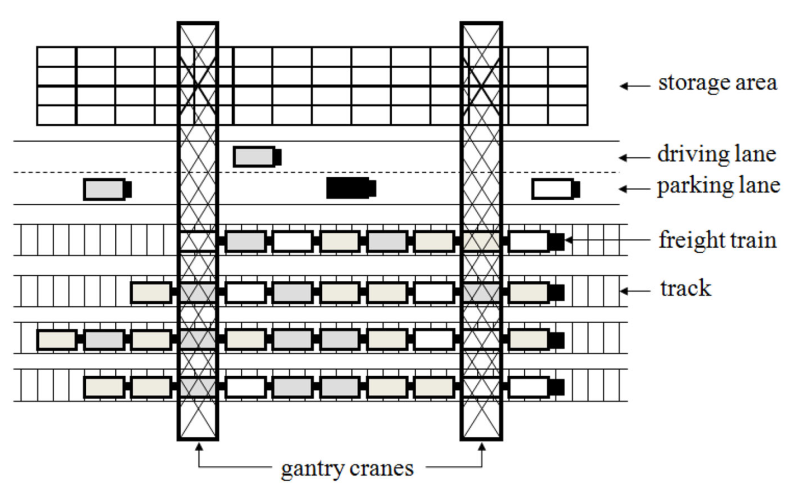
\includegraphics[width=\textwidth]{img/costs.png}
\caption{Schematische Darstellung eines Bahn-Terminals \cite{Briskorn2018}.}
\label{fig:costs}
\end{figure}
Die Transportkosten werden in einer Matrix $C = (c_{iq})_{n \times m}$ kodiert, \newline wobei $c_{iq} \coloneqq d_{man}(O_i, F_q)$.
D.h. der Eintrag an der Stelle $c_{iq}$ entspricht den Kosten für den Transport des \textit{Items} $i$ in den \textit{Stack} $q$.

%%%%%%%%%%%%%%%%%%%%%%%%%%%%%%%%%%%%%%%%%%%%%%%%%%%%%%%%%%%%%%%%%%%%%%%%%%%%%%%%%%%%%%%%%%%%%%%%%%%%
\pagebreak
%%%%%%%%%%%%%%%%%%%%%%%%%%%%%%%%%%%%%%%%%%%%%%%%%%%%%%%%%%%%%%%%%%%%%%%%%%%%%%%%%%%%%%%%%%%%%%%%%%%%

\section{Nebenbedingungen}
\label{sec:constraints}

\subsection{Stacking Restriktionen}
\label{sec:stacking_restrictions}

Es gibt in der Praxis vielfältige Gründe dafür, dass nicht jedes \textit{Item} auf jedes andere \textit{Item} gestapelt werden darf.
Aus diesen resultieren bestimmte Restriktionen, die z.B. wie folgt lauten:
\begin{itemize}
  \item schwerere \textit{Items} dürfen nicht auf leichteren \textit{Items} platziert werden
  \item größere \textit{Items} dürfen nicht auf kleineren \textit{Items} platziert werden
  \item \textit{Items} bestimmter Materialien oder Zielorte dürfen nicht aufeinander gestapelt werden
\end{itemize}

All jene Restriktionen, die im Folgenden stets als \textit{Stacking Constraints} bezeichnet werden, werden in einer Binärmatrix $S = (s_{ij})_{n \times n}$ kodiert, wobei:
\[
    s_{ij} =
\begin{cases}
    1, & \text{wenn $i$ direkt auf $j$ gestapelt werden darf }\\
    0, & \text{sonst}
\end{cases}
\]
Diese Matrix lässt sich, wie in Abb. \ref{fig:matrix_to_graph} beispielhaft dargestellt,
als gerichteter Graph mit $n$ Knoten für alle $i \in I$ und Kanten $i \rightarrow j$ für alle $s_{ij} = 1$ repräsentieren.
\begin{figure}[H]
  \begin{subfigure}[b]{0.5\textwidth}
  \centering
    $S =$
    $\left(
    \begin{array}{rrrr}
    0 & 1 & 1 & 0 \\
    1 & 0 & 1 & 0 \\
    1 & 0 & 0 & 0 \\
    1 & 1 & 1 & 0 \\
    \end{array} \right) $
    \caption{\textsc{Constraint Matrix}}
    \label{fig:constraint_matrix}
  \end{subfigure}
  \hfill
  \begin{subfigure}[b]{0.5\textwidth}
  \centering
    \begin{tikzpicture}[->, scale=0.50, transform shape, node distance=2.5cm]
    \node[state] (A) {1};
    \node[state] (B) [right of=A] {2};
    \node[state] (C) [below of=A] {3};
    \node[state] (D) [right of=C] {4};

    \path (A) edge node {} (B)
          (A) edge node {} (C)

          (B) edge [bend right] node {} (A)
          (B) edge [bend left=10] node {} (C)

          (C) edge [bend left] node {} (A)

          (D) edge [bend left=10] node {} (A)
          (D) edge node {} (B)
          (D) edge node {} (C);
  \end{tikzpicture}
    \caption{\textsc{Resultierender Graph}}
    \label{fig:resulting_graph}
  \end{subfigure}
  \caption{\textsc{Repräsentation der Stacking Constraints.}}
  \label{fig:matrix_to_graph}
\end{figure}
In dieser Arbeit werden ausschließlich transitive \textit{Stacking Constraints} betrachtet, d.h.
wenn \textit{Item} $i$ auf \textit{Item} $j$ und \textit{Item} $j$ auf \textit{Item} $h$ gestapelt werden darf,
so darf auch \textit{Item} $i$ auf \textit{Item} $h$ gestapelt werden.\newline
Diese Eigenschaft ist auch in der Praxis häufig gegeben.
Restriktionen bezüglich des Gewichts und der Länge haben die besondere Eigenschaft, dass alle Items vergleichbar sind, d.h. für alle $i \neq j  \quad \text{gilt} \quad s_{ij} = 1 \quad \text{oder} \quad s_{ji} = 1$, was bedeutet, dass diese Restriktionen eine totale Ordnung auf allen \textit{Items} definieren.

%%%%%%%%%%%%%%%%%%%%%%%%%%%%%%%%%%%%%%%%%%%%%%%%%%%%%%%%%%%%%%%%%%%%%%%%%%%%%%%%%%%%%%%%%%%%%%%%%%%%
\pagebreak
%%%%%%%%%%%%%%%%%%%%%%%%%%%%%%%%%%%%%%%%%%%%%%%%%%%%%%%%%%%%%%%%%%%%%%%%%%%%%%%%%%%%%%%%%%%%%%%%%%%%

\subsection{Placement Restriktionen}
\label{sec:placement_restrictions}

Die im Folgenden als \textit{Placement Constraints} bezeichneten Einschränkungen bezüglich der Position eines \textit{Items} resultieren z.B.
aus der Länge oder dem Gewicht der \textit{Items} und den Eigenschaften der \textit{Stacks}. Es gibt allerdings auch \textit{Items} mit speziellen Anforderungen, z.B. Kühlcontainer, die eine Energiequelle benötigen. Solche \textit{Items} können nur \textit{Stacks} mit entsprechender Konfiguration zugewiesen werden. Tendenziell sind dabei mehr \textit{Item}-\textit{Stack}-Zuweisungen erlaubt als verboten. Diese \textit{Placement Constraints} werden allerdings nicht direkt implementiert, sondern indirekt über hohe Kostenwerte.

Dies hat den Vorteil, dass die Placement Constraints zunächst nur \textquote{Weak Constraints} sind, d.h. es wird auch
dann eine Lösung gefunden, wenn gegen diese Nebenbedingungen verstoßen wird. Eine solche Lösung wird allerdings nur dann generiert,
wenn keine Lösung existiert, die sämtliche Placement Constraints respektiert.
Anschließend kann entschieden werden, ob solche Lösungen als zulässig gelten, oder, ob die Placement Constraints trotzdem
als \textquote{Hard Constraints} betrachtet und solche Lösungen dementsprechend unzulässig sind. Diese Art der Implementation ist sehr flexibel.

Der wesentliche Grund der Entscheidung für diese Art der Implementation ist allerdings eher pragmatischer Natur, denn der in den konstruktiven Heuristiken, die in Kapitel \ref{sec:constructive_heuristics} vorgestellt werden, verwendete Algorithmus zur Berechnung eines Minimum-Weight-Perfect-Matchings, erwartet einen vollständig bipartiten Graphen als Eingabe. Dies bedeutet, dass jedes Item zunächst mit jedem Stack kompatibel sein muss. Da die Placement Constraints genau dies jedoch verhindern, ist es sinnvoll, diese, wie im Folgenden beschrieben, indirekt über hohe Kostenwerte umzusetzen.

Zunächst werden die \textit{Placement Constraints} in einer Binärmatrix $T = (t_{iq})_{n \times m}$ kodiert, wobei:\newline
\[
    t_{iq} =
\begin{cases}
    1, & \text{wenn \textit{Item} $i$ in \textit{Stack} $q$ platziert werden darf }\\
    0, & \text{sonst}
\end{cases}
\]
Diese Matrix wird jedoch nicht direkt verwendet, um die Restriktionen zu implementieren. Stattdessen wird
die Transportkosten-Matrix $C = (c_{iq})_{n \times m}$, die in Abschnitt \ref{sec:transport_costs} eingeführt wurde, nun wie folgt erweitert.
\[
    c_{iq} =
\begin{cases}
    d_{man}(O_i, F_q), & \text{wenn $t_{iq} = 1$}\\
    \infty, & \text{sonst}
\end{cases}
\]
Der Eintrag an der Stelle $c_{iq}$ enthält also nur noch dann die tatsächlichen Transportkosten, wenn die
entsprechende \textit{Item}-\textit{Stack}-Zuweisung basierend auf den \textit{Placement Constraints} erlaubt ist und sonst $\infty$.

Die \textit{Placement Constraints} gelten als verletzt, wenn eine Lösung eine \textit{Item}-\textit{Stack}-Zuweisung der Kosten $\infty$ enthält.

%%%%%%%%%%%%%%%%%%%%%%%%%%%%%%%%%%%%%%%%%%%%%%%%%%%%%%%%%%%%%%%%%%%%%%%%%%%%%%%%%%%%%%%%%%%%%%%%%%%%
\pagebreak
%%%%%%%%%%%%%%%%%%%%%%%%%%%%%%%%%%%%%%%%%%%%%%%%%%%%%%%%%%%%%%%%%%%%%%%%%%%%%%%%%%%%%%%%%%%%%%%%%%%%

\section{Problemstellungen}
\label{sec:problem_settings}

In diesem Kapitel werden konkret die Problemstellungen eingeführt, die im Folgenden heuristisch gelöst werden.
Es werden die \textit{Stack}-Kapazitäten $b=2, b=3 $ und $ b=4$ betrachtet, die besonders in Szenarien aus der Praxis, in denen
es darum geht, Container zu stapeln, von Interesse sind.

\subsection{Komplexität}
\label{sec:complexity}

Wie \cite{Bruns2015} zeigte, handelt es sich bei dem Zulässigkeitsproblem mit einer \textit{Stack}-Kapazität von $b=3$ und gegebenen transitiven \textit{Stacking Constraints} $s_{ij}$ um ein stark NP-vollständiges Problem. Erst kürzlich wurde außerdem gezeigt, dass auch das Problem mit einer \textit{Stack}-Kapazität von $b=2$ mit gegebenen transitiven \textit{Stacking Constraints} $s_{ij}$ und \textit{Placement Constraints} $t_{iq}$ NP-vollständig ist. Diese Erkenntnis wurde allerdings noch nicht veröffentlicht. Somit sind auch die entsprechenden Stacking-Probleme, bei denen zusätzlich die Transportkosten minimiert werden, NP-vollständig. Für eben diese Probleme werden in dieser Arbeit heuristische Lösungsansätze präsentiert.

\subsection{Instanzgrößen}
\label{sec:instance_sizes}

Zu Testzwecken werden unterschiedlich große Instanzen von Stacking-Problemen generiert. Die Größe einer
Instanz bezieht sich dabei stets auf die Anzahl der betrachteten Items. Die Testinstanzen werden
in drei Kategorien unterteilt:
\begin{itemize}
  \item klein (\textbf{s}) ($\leq 100$ Items)
  \item mittelgroß (\textbf{m}) ($\approx 300$ Items)
  \item groß (\textbf{l}) ($\approx 500$ Items)\newline
\end{itemize}
Dies scheinen auch in der Literatur Größenordnungen zu sein, in dem sich praktisch motivierte Stacking-Probleme
typischerweise bewegen. \cite{Le2016}

\subsection{Zielfunktion}
\label{sec:objective}

Das Ziel, welches im Folgenden für sämtliche Problemstellungen angestrebt wird, ist eine möglichst günstige Einlagerung
sämtlicher \textit{Items}, d.h. die Zielfunktion entspricht der Minimierung der Transportkosten.
Dabei haben Zulässigkeit und geringe Laufzeit Priorität.
Eine Lösung wird dann als zulässig betrachtet, wenn sämtliche \textit{Items} unter Berücksichtigung der \textit{Stacking}- und \textit{Placement-Constraints} sowie der \textit{Stack}-Kapazität, eingelagert wurden.


%%%%%%%%%%%%%%%%%%%%%%%%%%%%%%%%%%%%%%%%%%%%%%%%%%%%%%%%%%%%%%%%%%%%%%%%%%%%%%%%%%%%%%%%%%%%%%%%%%%%
\pagebreak
%%%%%%%%%%%%%%%%%%%%%%%%%%%%%%%%%%%%%%%%%%%%%%%%%%%%%%%%%%%%%%%%%%%%%%%%%%%%%%%%%%%%%%%%%%%%%%%%%%%%

\section{Testdaten-Generierung}
\label{sec:test_data}

Um die entwickelten Lösungsverfahren testen und vergleichen zu können, werden Testinstanzen generiert,
die im Idealfall nicht allzu weit von realistischen Szenarien entfernt sein sollten.
Pro Konfiguration werden 20 Instanzen generiert, damit aussagekräftige Ergebnisse entstehen.

\textbf{Anzahl zur Verfügung stehender Stacks}

Die Anzahl der \textit{Items} $n$ sowie die \textit{Stack}-Kapazität $b$ wird stets spezifiziert und in der Berechnung der Anzahl
zur Verfügung stehender \textit{Stacks} $m$ verwendet. Es gilt $m$ = $\ceil{n / b}$ + $20 \%$.
Bei einer \textit{Stack}anzahl von $m$ = $\ceil{n / b}$ gäbe es überhaupt keinen Spielraum bei der \textit{Item}platzierung. Aufgrund der in Abschnitt \ref{sec:constraints} geschilderten Nebenbedingungen wären die meisten Instanzen dann jedoch unlösbar.
Daher wurde zunächst ein durchaus geringer Spielraum von $20 \%$ eingeführt, der in weiteren Betrachtungen erhöht werden könnte.

\textbf{Stacking Constraints}

Es wurden zwei Varianten der \textit{Stacking-Constraint}-Generierung implementiert, die jeweils spezifische Vor- und Nachteile aufweisen.

\textbf{Variante 1}

Die \textit{Stacking-Constraint}-Matrix $S$ wird anhand einer definierten Wahrscheinlichkeit mit $1$- bzw. $0$-Einträgen gefüllt.
Anschließend werden die $1$-Einträge, die aus Transitivität folgen, ergänzt.

\textbf{Variante 2}

Für alle $n$ \textit{Items} wird eine zufällige Länge und Breite generiert. \textit{Item} $i$ kann auf \textit{Item} $j$ platziert werden,
wenn für dessen Länge $l_i$ und Breite $w_i$ gilt $l_i \leq l_j$ und $w_i \leq w_j$.
Zwei \textit{Items} $i, j$ sind in beide Richtungen stackbar, wenn $l_i = l_j$ und $w_i = w_j$ gilt.

Variante 2 scheint realitätsnäher zu sein und wird deshalb zunächst bevorzugt. Aufgrund der Tatsache, dass Variante 2 jedoch stets
zu einem Anteil von $1$-Einträgen in der Matrix von ca. $25\%$ führt und dieser mit Variante 1 sehr gut konfigurierbar ist, wird Variante 1 nicht verworfen. (TODO: Grund ergänzen...)

\textbf{Placement Constraints}

Die Placement Constraints werden zufällig generiert, wobei die Wahrscheinlichkeit für $t_{iq} = 1$, also dafür,
dass ein Item $i$ in einem Stack $q$ platziert werden darf, $70 \%$ beträgt, da, wie in Kapitel \ref{sec:placement_restrictions} bereits erwähnt, tendenziell mehr Zuweisungen erlaubt als verboten sind.

\textbf{Transportkosten}

Zur Transportkostenberechnung wird, wie in Abschnitt \ref{sec:transport_costs} erläutert, die Manhattan-Metrik verwendet. Dazu sind
entsprechend die \textit{Item}- und \textit{Stack}positionen als $x$- und $y$-Koordinaten gegeben. Auch die entsprechenden Längen und Breiten sowie die Distanz zwischen \textit{Storage-Area} und den Fahrzeug-Lanes ist jeweils gegeben.

%%%%%%%%%%%%%%%%%%%%%%%%%%%%%%%%%%%%%%%%%%%%%%%%%%%%%%%%%%%%%%%%%%%%%%%%%%%%%%%%%%%%%%%%%%%%%%%%%%%%
\pagebreak
%%%%%%%%%%%%%%%%%%%%%%%%%%%%%%%%%%%%%%%%%%%%%%%%%%%%%%%%%%%%%%%%%%%%%%%%%%%%%%%%%%%%%%%%%%%%%%%%%%%%

\section{MIP-Formulierungen}
\label{sec:mip_formulations}

In diesem Kapitel werden MIP-Formulierungen eingeführt, die dem experimentellen Vergleich dienen.
Diese werden verwendet, um die optimalen Zielfunktionswerte der Test-Instanzen zu ermitteln und somit eine Grundlage zu schaffen, mit der die Qualität der von den Heuristiken generierten Lösungen beurteilt werden kann. Des Weiteren geht es auch um einen Vergleich der im Folgenden vorgestellten MIP-Formulierungen untereinander. Zunächst wird in Abschnitt \ref{sec:mip_definition} kurz die Idee des MIP im Allgemeinen
eingeführt, um dann im Anschluss in den Abschnitten \ref{sec:bin_packing_formulation} und \ref{sec:three_idx_formulation} die beiden in dieser Arbeit betrachteten MIP-Formulierungen im Detail vorzustellen.

\subsection{Mixed Integer Linear Programming (MIP)}
\label{sec:mip_definition}

Viele kombinatorische Optimierungsprobleme lassen sich als lineare Programme formulieren, die sich dadurch
auszeichnen, dass die Zielfunktion eine lineare Funktion in Abhängigkeit von den Entscheidungsvariablen ist
und alle Nebenbedingungen in Form von linearen Gleichungen und Ungleichungen vorliegen. Für diese Probleme gibt es mit dem Simplexverfahren ein sehr effizientes Lösungsverfahren.\cite{Knust2017}

Ein gemischt-ganzzahliges lineares Programm (MIP) ist ein lineares Programm, welches kontinuierliche und ganzzahligen Variablen
enthält. Im Gegensatz zur kontinuierlichen Variante, ist die Lösung von ganzzahligen linearen Programmen NP-schwer.
Während sogar sehr große kontinuierliche lineare Programme durch kommerzielle Solver in wenigen Minuten gelöst werden können, gilt dies nicht für ganzzahlige lineare Programme. Diese können nur mit deutlich zeitaufwändigeren Algorithmen wie Branch \& Bound gelöst werden.\cite{Brucker2006}

In dieser Arbeit wird das Java-Interface von CPLEX, einem Solver für lineare Optimierungsprobleme verwendet,
um die MIP-Formulierungen, die in Abschnitt \ref{sec:bin_packing_formulation} und Abschnitt \ref{sec:three_idx_formulation} vorgestellt werden,
zu lösen. Es handelt sich dabei um eine unter anderem auf dem Simplexverfahren basierende Implementation von IBM. \cite{CPLEX2015}

\subsection{Bin-Packing-Formulierung}
\label{sec:bin_packing_formulation}

Die Bin-Packing-Formulierung orientiert sich dem Namen nach am klassichen \textsc{Bin-Packing} Problem, bei dem es darum geht,
eine Menge von Objekten so auf eine Menge von Behältern zu verteilen, dass die Behälterkapazitäten eingehalten werden.
Dies beschreibt auch direkt den Ansatz der Bin-Packing-Formulierung. Die Stacks werden als Behälter betrachtet und die Items als Objekte,
die diesen Behältern zugeordnet werden, wobei die Behälter- bzw. Stack-Kapazität jeweils eingehalten wird. Im Unterschied zum klassischen \textsc{Bin-Packing} müssen zusätzlich die Stacking- und Placement-Constraints berücksichtigt werden.

\pagebreak

Es sei eine Menge von Items $I = \{1, ..., n\}$ und eine Menge von Stacks $Q = \{1, ..., m\}$ mit einer Kapazität von $b$ gegeben.
Außerdem sei $G = (I, A)$ ein transitiver Stacking-Constraint-Graph, bei dem eine Kante $(i, j) \in A$ bedeutet,
dass die Items $i$ und $j$ in mindestens einer Richtung stackbar sind, also $s_{ij} = 1$ oder $s_{ji} = 1$.\newline
Bei den Variablen $x_{iq}$ handelt es sich um Binärvariablen, wobei $x_{iq} = 1$ bedeutet, dass Item $i$ Stack $q$ zugewiesen wird.
Die Kosten werden über die Variablen $c_{iq}$ modelliert, wobei $c_{iq}$ den Kosten für den Transport des Items $i$ in den Stack $q$
entspricht.

\begin{gather}
\boldsymbol{min} \quad \sum_{i \in I} \sum_{q \in Q} c_{iq} x_{iq} \label{bin_packing_line_one} \\
\thinspace\thinspace \boldsymbol{s.t.} \thinspace\quad\thinspace\thinspace\thinspace\quad\thinspace \quad \sum_{q \in Q} x_{iq} = 1 \quad\quad\quad\quad\quad\quad\quad \forall i \in I \quad\quad\quad\quad\thinspace\thinspace \label{bin_packing_line_two} \\
\quad \sum_{i \in I} x_{iq} \leq b \quad\quad\quad\quad\quad\quad\quad \forall q \in Q \label{bin_packing_line_three} \\
\thinspace\thinspace\quad\quad x_{iq} + x_{jq} \leq 1 \quad\quad\thinspace\thinspace\quad\quad\quad\quad \forall \{i, j\} \notin A \label{bin_packing_line_four} \\
\thinspace\thinspace\quad\quad\quad x_{iq} \in \{0, 1\} \thinspace\thinspace\thinspace\thinspace\thinspace\thinspace\quad\quad\quad\quad\quad\quad \forall i \in I, q \in Q \thinspace \label{bin_packing_line_five}
\end{gather}

In (\ref{bin_packing_line_one}) wird die betrachtete Zielfunktion definiert, welche die Summe der Kosten sämtlicher
Item-Stack-Zuweisungen minimiert, was der Minimierung der Transportkosten entspricht.
Nebenbedingung (\ref{bin_packing_line_two}) fordert, dass jedes Item genau einem Stack zugewiesen wird. Die Ungleichung in (\ref{bin_packing_line_three}) entspricht der Forderung, dass für sämtliche Stacks die Stack-Kapazität eingehalten werden muss, d.h.
die Summe der eines Stacks zugewiesenen Items darf dessen Kapazität nicht überschreiten. (\ref{bin_packing_line_four}) entspricht schließlich der Forderung, dass alle Items, die nicht stackbar sind, für die also keine Kante im Stacking-Constraint-Graph existiert, nicht Teil desselben Stacks sind. Außerdem handelt es sich laut (\ref{bin_packing_line_five}), wie bereits erwähnt, bei den Variablen $x_{iq}$ um Binärvariablen.

\subsection{3-Index-Formulierung}
\label{sec:three_idx_formulation}

Die 3-Index-Formulierung enthält drei Indizes - Item, Stack und Level.
Im Gegensatz zur Bin-Packing-Formulierung, die Item-Stack-Zuweisungen vornimmt, weist die 3-Index-Formulierung einem
Item auch eine konkrete Position innerhalb eines Stacks zu, sie berücksichtigt also den Level.

Gegeben sei erneut eine Item-Menge $I = \{1, ..., n\}$ und eine Stack-Menge $Q = \{1, ..., m\}$, die Stacks der Kapazität $b$ enthält.
Jeder Stack enthält dementsprechend die Level $L = \{1, ..., b\}$. Des Weiteren sei ein transitiver Stacking-Constraint-Graph
$G = (I, A)$ gegeben, bei dem eine Kante $i \rightarrow j \in A$ bedeutet, dass das Item $i$ direkt auf das Item $j$ gestapelt werden darf.
Die Kosten seien durch die gegebene Transportkostenmatrix $C$ definiert, in der an der Stelle $c_{iq}$ die Kosten für den
Transport von Item $i$ in Stack $q$ stehen. Bei den Variablen $x_{iql}$ handelt es sich um Binärvariablen,
bei denen $x_{iql} = 1$ bedeutet, dass Item $i$ in Stack $q$ auf Level $l$ platziert wird.

\begin{gather}
\boldsymbol{min} \quad \sum_{i \in I} \sum_{q \in Q} \sum_{l \in L} c_{iq} x_{iql} \label{three_idx_line_one} \\
\boldsymbol{s.t.} \quad \sum_{q \in Q} \sum_{l \in L} x_{iql} = 1 \quad\thinspace\thinspace\quad\quad\quad\quad \forall i \in I \thinspace\thinspace\quad\quad\quad\quad\quad\quad\quad\quad\thinspace\thinspace \label{three_idx_line_two} \\
\sum_{i \in I} x_{iql} \leq 1 \thinspace\quad\quad\quad\quad\quad\quad\quad \forall q \in Q, l \in L \thinspace\thinspace\thinspace\thinspace\quad\quad\quad\thinspace \label{three_idx_line_three} \\
\sum_{j \in I | i \rightarrow j \in A} x_{jq(l-1)} - x_{iql} \geq 0 \thinspace\quad\quad \forall i \in I, q \in Q, l \in L \textbackslash \{1\}
\label{three_idx_line_four} \\
\quad\quad x_{iql} \in \{0, 1\} \quad\quad\quad\quad\quad\quad\quad \forall i \in I, q \in Q, l \in L \quad\thinspace\thinspace\thinspace\thinspace\thinspace \label{three_idx_line_five}
\end{gather}

In (\ref{three_idx_line_one}) wird die Zielfunktion definiert, die erneut die Summe der Kosten sämtlicher Item-Zuweisungen
und somit die Transportkosten minimiert.
Nebenbedingung (\ref{three_idx_line_two}) fordert, dass sich jedes Item in genau einem Stack an genau einer Position (Level) befindet.
Anschließend wird in (\ref{three_idx_line_three}) gefordert, dass sich an jeder Position in jedem Stack höchstens ein Item befindet und
(\ref{three_idx_line_four}) formuliert die Einschränkung, dass jedes Item, welches oberhalb des Ground-Levels platziert wird,
ein Item unter sich hat, welches sich basierend auf den Stacking Constraints dort befinden darf. Schließlich wird in (\ref{three_idx_line_five}) festgehalten, dass es sich bei den $x_{iql}$ um Binärvariablen handelt.

Beide Formulierungen weisen jedem Item einen Stack zu und minimieren dabei die Transportkosten.
Die Bin-Packing-Formulierung nimmt dabei lediglich Item-Stack-Zuweisungen vor, während die 3-Index-Formulierung die
Items konkreten Positionen innerhalb der Stacks zuweist. Dabei ist allerdings auch bei der Bin-Packing-Formulierung
sichergestellt, dass eine Item-Stack-Zuweisung nur dann vorgenommen wird, wenn die Items innerhalb des Stacks anschließend
in einer Weise umsortiert werden können, dass sie den Stacking Constraints entsprechen. Diese Tatsache ergibt sich aus Nebenbedingung (\ref{bin_packing_line_four}), welche fordert, dass Items sich nur dann im selben Stack befinden, wenn sie in mindestens einer Richtung stackbar sind.
Da die Stacking Constraints außerdem transitiv sind, ist sichergestellt, dass die Reihenfolge innerhalb der Stacks stets so korrigiert
werden kann, dass eine valide Lösung, die die Stacking Constraints respektiert, dabei herauskommt.

Die 3-Index-Formulierung liefert folglich direkt eine zulässige Lösung, während die Item-Stack-Zuweisungen, die die Bin-Packing-Formulierung liefert, zunächst noch sortiert werden müssen, damit sie eine zulässige Lösung ergeben. Dies kann durch den simplen Algorithmus \ref{alg:algo1} erreicht werden.

\begin{algorithm}
\fontsize{10pt}{10pt}

\SetAlgoLined

  \ForEach{stack in storageArea}{

    somethingChanged = true\;

    \While{somethingChanged}{

      somethingChanged = false\;

      \For{position = 0; position < stack.capacity - 1; position++}{
          \BlankLine\BlankLine
          \uIf{stack[position].\Call{isOccupied()}{} \&\& stack[position + 1].\Call{isOccupied()}{{}}}{
            \uIf{itemAt(stack[position]).\Call{isStackableOn}{itemAt(stack[position + 1])}}{

                \Call{exchangeItems}{stack[position], stack[position + 1]}\;
                somethingChanged = true\;
                break\;
            }
          }
      }
    }
  }

\caption{Korrektur der Item Reihenfolge innerhalb der Stacks.}
\label{alg:algo1}
\end{algorithm}

%%%%%%%%%%%%%%%%%%%%%%%%%%%%%%%%%%%%%%%%%%%%%%%%%%%%%%%%%%%%%%%%%%%%%%%%%%%%%%%%%%%%%%%%%%%%%%%%%%%%
\pagebreak
%%%%%%%%%%%%%%%%%%%%%%%%%%%%%%%%%%%%%%%%%%%%%%%%%%%%%%%%%%%%%%%%%%%%%%%%%%%%%%%%%%%%%%%%%%%%%%%%%%%%

\section{Konstruktive Heuristiken}
\label{sec:constructive_heuristics}

In diesem Abschnitt werden die entwickelten konstruktiven Heuristiken zur Lösung der in Kapitel \ref{sec:problem_settings}
beschriebenen Problemstellungen vorgestellt.
Zunächst werden drei wichtige Konzepte eingeführt, die in den Heuristiken Verwendung finden.
In \ref{sec:digression_mcm} Maximum-Cardinality-Matchings,
in \ref{sec:digression_mwpm} Minimum-Weight-Perfect-Matchings und in \ref{sec:digression_bipartite_graph}
bipartite Graphen. Anschließend geht es in \ref{sec:two_cap_heuristic} um die konstruktive Heuristik für eine Stack-Kapazität
von $b=2$ und darauffolgend in \ref{sec:solver_comp_b=2} um einen Vergleich der Solver für eben diese Stack-Kapazität.
In \ref{sec:three_cap_heuristic} geht es dann um die konstruktive Heuristik für eine Stack-Kapazität von $b=3$, auf
die erneut ein Vergleich der entsprechenden Solver in \ref{sec:solver_comp_b=3} folgt.

\subsection{Exkurs: Maximum-Cardinality-Matching (MCM)}
\label{sec:digression_mcm}

Gegeben sei ein ungerichteter Graph $G = (V, E)$. Eine Menge $M \subseteq E$ heißt Matching,
wenn keine zwei Kanten aus $M$ einen Knoten gemeinsam haben. Falls $M$ als Menge eine maximale Kardinalität unter
allen Matchings von $G$ hat, wird dies als Maximum-Cardinality-Matching bezeichnet. \cite{WikiMatching}
Es kann mehrere unterschiedliche MCMs in einem Graphen geben.
In Abb. \ref{fig:mcm_examples} sind beispielhaft zwei MCMs dargestellt.
\begin{figure}[H]
  \begin{subfigure}[b]{0.4\textwidth}
  \centering
    \begin{tikzpicture}[scale=0.45, transform shape, node distance=2cm]
    \node[state] (A) {};
    \node[state] (B) [above right of=A] {};
    \node[state] (C) [below left of=A] {};
    \node[state] (D) [below right of=C] {};
    \node[state] (F) [below right of=B] {};
    \node[state] (E) [below of=F] {};

    \path (A) edge [red] node {} (B)
          (A) edge node {} (C)
          (A) edge node {} (D)
          (A) edge node {} (E)
          (A) edge node {} (F)
          (C) edge [red] node {} (D);
  \end{tikzpicture}
  \caption{\textsc{$|MCM| = 2$}}
  \label{fig:mcm1}
  \end{subfigure}
  \hfill
  \begin{subfigure}[b]{0.4\textwidth}
  \centering
    \begin{tikzpicture}[scale=0.45, transform shape, node distance=2cm]
    \node[state] (A) {};
    \node[state] (B) [right of=A] {};
    \node[state] (C) [right of=B] {};
    \node[state] (D) [below left of=A] {};
    \node[state] (E) [below right of=D] {};
    \node[state] (F) [right of=E] {};

    \path (A) edge node {} (B)
          (B) edge [red] node {} (C)
          (B) edge node {} (F)
          (A) edge node {} (E)
          (E) edge [red] node {} (F)
          (A) edge [red] node {} (D)
          (D) edge node {} (E);
  \end{tikzpicture}
    \caption{\textsc{$|MCM| = 3$}}
    \label{fig:mcm_2}
  \end{subfigure}
  \caption{\textsc{Beispiele für MCMs (dargestellt in rot).}}
  \label{fig:mcm_examples}
\end{figure}

\subsection{Exkurs: Minimum-Weight-Perfect-Matching}
\label{sec:digression_mwpm}

Bei einem Perfect-Matching handelt es sich um ein Matching, welches sämtliche Knoten des Graphen matcht.
Jeder Knoten des Graphen ist dabei inzident zu genau einer Kante des Matchings (vgl. Abb. \ref{fig:perfect_matching}).
Daher ist ein Perfect-Matching nur für Graphen mit einer geraden Anzahl an Knoten möglich.
Ein Minimum-Weight-Perfect-Matching ist nun ein günstigstes Perfect-Matching basierend auf den Kantenkosten.
\begin{figure}[H]
\centering
\begin{tikzpicture}[-, scale=0.6, transform shape, node distance=3cm]
    \node[state] (A) {};
    \node[state] (B) [above right of=A] {};
    \node[state] (C) [below right of=A] {};
    \node[state] (D) [right of=B] {};
    \node[state] (E) [right of=D] {};
    \node[state] (F) [right of=C] {};

    \path (A) edge [red] node {} (B)
          (A) edge node {} (C)
          (B) edge node {} (D)
          (B) edge node {} (C)
          (D) edge [red] node {} (E)
          (D) edge node {} (F)
          (C) edge [red] node {} (F);
\end{tikzpicture}
\caption{\textsc{Beispiel für ein Perfect-Matching (rot).}}
\label{fig:perfect_matching}
\end{figure}

\subsection{Exkurs: Bipartiter Graph}
\label{sec:digression_bipartite_graph}

Ein Graph $G = (V, E)$ heißt bipartit (vgl. Abb. \ref{fig:digression_bipartite_graph}), wenn die Knotenmenge in zwei disjunkte Teilmengen zerfällt
$(V = S \cup T$ mit $S \cap T = \emptyset$), sodass jede Kante einen Knoten aus $S$ mit einem Knoten aus $T$ verbindet. \cite{HochschuleDarmstadt}\newline
Es lassen sich folgende Äquivalenzen \cite{Leighton2010} festhalten:
\begin{itemize}
  \item $G$ bipartit $\iff$ $G$ 2-färbbar
  \item $G$ bipartit $\iff$ keine Kreise ungerader Länge in $G$
\end{itemize}
In Abb. \ref{fig:digression_bipartite_graph} ist die 2-Färbbarkeit eines bipartiten Graphen, bei der die eine Teilmenge
in grün und die andere Teilmenge in rot gefärbt ist, visualisiert. Man kann daran gut erkennen, dass es in solchen Graphen
ausschließlich Kanten gibt, die einen Knoten der einen Teilmenge (rot) mit einem Knoten der anderen Teilmenge (grün) verbinden,
jedoch keine Kanten zwischen Knoten derselben Farbe bzw. Teilmenge.

\begin{figure}[H]
\centering
\begin{tikzpicture}[scale=0.6, transform shape, node distance=3cm]
  \node[state] [green] (A) {};
  \node[state] [red] (B) [above right of=A] {};
  \node[state] [green] (C) [below right of=B] {};
  \node[state] [red] (D) [below of=B] {};
  \node[state] [red] (E) [below of=A] {};
  \node[state] [green] (F) [right of=E] {};

  \path (A) edge node {} (B)
        (B) edge node {} (C)
        (C) edge node {} (D)
        (A) edge node {} (D)
        (A) edge node {} (E)
        (E) edge node {} (F)
        (D) edge node {} (F);

\end{tikzpicture}
\caption{\textsc{Bipartiter Graph.}}
\label{fig:digression_bipartite_graph}
\end{figure}

\subsection{Konstruktive Heuristik ($b = 2$)}
\label{sec:two_cap_heuristic}

In diesem Abschnitt wird eine konstruktive Heuristik zur Lösung von Stacking-Problemen mit Stacks der Kapazität $b=2$
vorgestellt.

Zunächst wird ein Stacking-Constraint-Graph $G = (V, E)$ generiert, welcher die Items als Knoten enthält, d.h. $V = I$. Dieser Graph
enthält eine Kante $\{i, j\}$ zwischen zwei Knoten, wenn die entsprechenden Items $i, j \in I$ in mindestens einer Richtung stackbar sind, d.h.
wenn $s_{ij} + s_{ji} \geq 1$.

Berechnet man nun ein \textsc{MCM} in $G$ und interpretiert dessen Kanten als Stacks, welche die beiden Knoten, die durch
die Kanten verbunden werden, als Items enthalten, so erhält man die größtmögliche Anzahl von vollständig gefüllten Stacks.
Die Items, die nicht gematcht werden, werden auf dem Ground-Level platziert.
Insgesamt werden auf diese Weise so wenig Stacks wie möglich verwendet.
Eine zulässige Lösung mit maximal $m$ Stacks kann nur dann existieren, wenn die Anzahl der Kanten im Matching plus der Anzahl der nicht gematchten Knoten nicht größer ist als $m$. Da die Anzahl der Knoten $n$ beträgt, kann ein \textsc{MCM} in der Laufzeit $O(n^{2.5})$ berechnet werden, wie Even und Kariv bereits 1975 zeigten.

Dies entspricht dem Vorgehen aus dem Beweis zu Theorem 1 aus dem Paper "Complexity Results for Storage Loading Problems with Stacking Constraints", welches 2015 von Bruns et al. veröffentlicht wurde.

Augrund der Placement Constraints kann allerdings nicht jedes Item in jedem Stack platziert werden, weshalb noch die bestmögliche Zuweisung von
Items- und Item-Paaren zu Stacks gefunden werden muss. Diese entspricht einer Zuweisung, in der sämtliche Items möglichst günstig einem Stack zugeordnet werden. Dazu wird ein bipartiter Graph $G_1 = (V_1 \cup V_2, A)$ generiert, wobei die Partition $V_1$ den Items bestehend aus Item-Paaren und Unmatched Items entspricht und $V_2$ den zur Verfügung stehenden Stacks.

Für alle $i \in V_1$ und $q \in V_2$ existiert eine Kante $\{i, q\} \in A$. Das Gewicht $c_{iq}$ dieser Kante ist definiert als die Kosten
des Transports des Items $i$ von seiner Originalposition $O_i$ zum Stack $q$.

Nun wird ein \textsc{MWPM} in $G_1$ berechnet, dessen Kanten als Stackzuweisungen interpretiert werden.
Da es sich um ein Perfect-Matching handelt, werden sämtliche Items einem Stack zugewiesen. Die Minimum-Weight-Variante eines
Perfect-Matchings sorgt dafür, dass es sich um eine günstigste Zuweisung sämtlicher Items zu Stacks handelt, da die Kantenkosten
den Transportkosten der Items entsprechen. Sollte kein \textsc{MWPM} existieren, so existiert auch keine zulässige Zuweisung
der generierten Item-Paare und Unmatched Items zu den Stacks, welche die Placement Constraints respektiert.
Abschließend muss ggf. die Reihenfolge innerhalb der Stacks angepasst werden, da für die Item-Paare bisher nur sichergestellt ist,
dass sie kompatibel und somit in mindestens einer Richtung stackbar sind. Die Richtung, in welcher sie stackbar sind, wurde bei der Zuweisung
jedoch noch nicht berücksichtigt.

\pagebreak

\textbf{Beispiel}

Gegeben sei die Item-Menge $I = \{0, 1, 2, 3, 4, 5, 6\}$ sowie eine Stack-Kapazität von $b = 2$.
Die Anzahl der zur Verfügung stehenden Stacks wird nun, wie in Abschnitt \ref{sec:test_data} geschildert,
durch $m = \ceil{n / b} + 20 \%$ berechnet und entspricht somit $m = \ceil{7 / 2} + 20 \% = 4$.

Die Stacking-Constraint-Matrix $S$ wird ebenfalls, wie in Abschnitt \ref{sec:test_data} beschrieben, generiert.
Basierend auf dieser wird der in Abb. \ref{fig:stacking_const_graph_example_b=2_a} dargestellte Stacking-Constraint-Graph
für die gegebenen Items generiert, auf welchem anschließend das in Abb. \ref{fig:stacking_const_graph_example_b=2_b} in grün dargestellte
\textsc{MCM} berechnet wird. Das in rot dargestellte Item 0 bleibt dabei unmatched.
\begin{figure}[H]
  \centering
    \begin{subfigure}[b]{0.4\textwidth}
    \centering
    \begin{tikzpicture}[scale=0.75, transform shape, node distance=3cm]
        \node[state] (G) [thick] {$\boldsymbol{6}$};
        \node[state] (B) [thick, above left of=G] {$\boldsymbol{1}$};
        \node[state] (C) [thick, above right of=G] {$\boldsymbol{2}$};
        \node[state] (E) [thick, below right of=G] {$\boldsymbol{4}$};
        \node[state] (F) [thick, below left of=G] {$\boldsymbol{5}$};
        \node[state] (A) [thick, below left of=B] {$\boldsymbol{0}$};
        \node[state] (D) [thick, below right of=C] {$\boldsymbol{3}$};

        \path (B) edge [thick] node {} (C)
              (B) edge [thick] node {} (F)
              (B) edge [thick] node {} (G)
              (C) edge [thick, bend right = 75, distance=5cm] node {} (F)
              (C) edge [thick] node {} (E)
              (C) edge [thick] node {} (D)
              (C) edge [thick] node {} (G)
              (F) edge [thick] node {} (G)
              (F) edge [thick] node {} (E)
              (E) edge [thick] node {} (G);
    \end{tikzpicture}
    \caption{\textsc{Stacking-Constraint-Graph}}
    \label{fig:stacking_const_graph_example_b=2_a}
    \end{subfigure}
    \hfill
    \begin{subfigure}[b]{0.4\textwidth}
    \centering
    \begin{tikzpicture}[scale=0.75, transform shape, node distance=3cm]
        \node[state] (G) [thick] {$\boldsymbol{\textcolor{mygreen}{6}}$};
        \node[state] (B) [thick, above left of=G] {$\boldsymbol{\textcolor{mygreen}{1}}$};
        \node[state] (C) [thick, above right of=G] {$\boldsymbol{\textcolor{mygreen}{2}}$};
        \node[state] (E) [thick, below right of=G] {$\boldsymbol{\textcolor{mygreen}{4}}$};
        \node[state] (F) [thick, below left of=G] {$\boldsymbol{\textcolor{mygreen}{5}}$};
        \node[state] (A) [thick, below left of=B] {$\boldsymbol{\textcolor{red}{0}}$};
        \node[state] (D) [thick, below right of=C] {$\boldsymbol{\textcolor{mygreen}{3}}$};

        \path (B) edge [thick] node {} (C)
              (B) edge [thick] node {} (F)
              (B) edge [thick, mygreen] node {} (G)
              (C) edge [thick, bend right = 75, distance=5cm] node {} (F)
              (C) edge [thick] node {} (E)
              (C) edge [thick, mygreen] node {} (D)
              (C) edge [thick] node {} (G)
              (F) edge [thick] node {} (G)
              (F) edge [thick, mygreen] node {} (E)
              (E) edge [thick] node {} (G);
    \end{tikzpicture}
    \caption{\textsc{MCM (Item $0$ unmatched)}}
    \label{fig:stacking_const_graph_example_b=2_b}
    \end{subfigure}
    \caption{}
    \label{fig:stacking_const_graph_example_b=2}
\end{figure}

Die Kanten des in Abb. \ref{fig:stacking_const_graph_example_b=2_b} in grün dargestellten \textsc{MCM} werden nun,
wie in Abb. \ref{fig:item_pairs_b=2} dargestellt, als kompatible Item-Paare interpretiert.
Item $0$ verbleibt dabei als einziges Unmatched Item.

\begin{figure}[H]
\centering
\begin{tikzpicture}[scale=0.7, transform shape, node distance=3cm]
        \node[state] (A) [thick] {\textcolor{mygreen}{$\boldsymbol{1, 6}$}};
        \node[state] (B) [thick, right of=A] {\textcolor{mygreen}{$\boldsymbol{2, 3}$}};
        \node[state] (C) [thick, right of=B] {\textcolor{mygreen}{$\boldsymbol{4, 5}$}};
        \node[state] (D) [thick, right of=C] {\textcolor{red}{$\boldsymbol{0}$}};
        \path ;
  \end{tikzpicture}
  \caption{\textsc{Resultierende Item-Paare.}}
  \label{fig:item_pairs_b=2}
\end{figure}

Nun geht es darum, eine Zuweisung der Item-Paare und Unmatched Items zu Stacks zu finden, welche die Placement Constraints
respektiert. Dazu wird zunächst der vollständig bipartite Graph in Abb. \ref{fig:bipartite_graph} generiert, welcher
die Items in der einen Partition und die Stacks in der anderen Partition enthält.
Dieser Graph ist, wie in Kapitel \ref{sec:placement_restrictions} erläutert, vollständig bipartit, da die Placement Constraints indirekt
über hohe Kostenwerte umgesetzt werden. Eine Zuweisung, die den Placement Constraints widerspricht, wird im \textsc{MWPM}
nur dann vorgenommen, wenn keine günstigere Variante existiert, d.h., wenn eine solche Zuweisung vollführt wird,
dann existiert keine Lösung, die sämtliche Placement Constraints respektiert.

\pagebreak

Das im bipartiten Graphen berechnete \textsc{MWPM} ist in Abb. \ref{fig:mwpm_b=2} dargestellt. Jede
Kante entspricht dabei der Zuweisung eines Item-Paars bzw. Unmatched Items zu einem Stack.
Die entsprechende Interpretation als zulässige Stack-Zuweisungen ist in Abb. \ref{fig:stacking_solution} visualisiert.

\begin{figure}[H]
\begin{subfigure}[b]{0.45\textwidth}
\centering
\begin{tikzpicture}[scale=0.7, transform shape, node distance=1.5cm]
        \node[state] (A) [thick] {$\boldsymbol{1, 6}$};
        \node[state] (B) [thick, below of=A] {$\boldsymbol{2, 3}$};
        \node[state] (C) [thick, below of=B] {$\boldsymbol{4, 5}$};
        \node[state] (D) [thick, below of=C] {$\boldsymbol{0}$};

        \node[state] (F) [thick, right = 4cm of A] {$\boldsymbol{S_1}$};
        \node[state] (G) [thick, right = 4cm of B] {$\boldsymbol{S_2}$};
        \node[state] (H) [thick, right = 4cm of C] {$\boldsymbol{S_3}$};
        \node[state] (I) [thick, right = 4cm of D] {$\boldsymbol{S_4}$};

        \path
          % from (1,6) to all stacks
          (A) edge [thick] node {} (F)
          (A) edge [thick] node {} (G)
          (A) edge [thick] node {} (H)
          (A) edge [thick] node {} (I)

          % from (2,3) to all stacks
          (B) edge [thick] node {} (F)
          (B) edge [thick] node {} (G)
          (B) edge [thick] node {} (H)
          (B) edge [thick] node {} (I)

          % from (4,5) to all stacks
          (C) edge [thick] node {} (F)
          (C) edge [thick] node {} (G)
          (C) edge [thick] node {} (H)
          (C) edge [thick] node {} (I)

          % from 0 to all stacks
          (D) edge [thick] node {} (F)
          (D) edge [thick] node {} (G)
          (D) edge [thick] node {} (H)
          (D) edge [thick] node {} (I);
  \end{tikzpicture}
  \caption{\textsc{vollständig bipartit}}
  \label{fig:bipartite_graph}
\end{subfigure}
\hfill
\begin{subfigure}[b]{0.45\textwidth}
\centering
\begin{tikzpicture}[scale=0.7, transform shape, node distance=1.5cm]
        \node[state] (A) [thick] {$\boldsymbol{1, 6}$};
        \node[state] (B) [thick, below of=A] {$\boldsymbol{2, 3}$};
        \node[state] (C) [thick, below of=B] {$\boldsymbol{4, 5}$};
        \node[state] (D) [thick, below of=C] {$\boldsymbol{0}$};

        \node[state] (F) [thick, right = 4cm of A] {$\boldsymbol{S_1}$};
        \node[state] (G) [thick, right = 4cm of B] {$\boldsymbol{S_2}$};
        \node[state] (H) [thick, right = 4cm of C] {$\boldsymbol{S_3}$};
        \node[state] (I) [thick, right = 4cm of D] {$\boldsymbol{S_4}$};

        \path
          (A) edge [thick] node {} (I)
          (B) edge [thick] node {} (H)
          (C) edge [thick] node {} (G)
          (D) edge [thick] node {} (F);
  \end{tikzpicture}
  \caption{\textsc{MWPM}}
  \label{fig:mwpm_b=2}
\end{subfigure}
\caption{}
\end{figure}

\begin{figure}[H]
  \centering
  \resizebox{0.4\textwidth}{!}{
    \begin{tabular}{c|c|c|c|c|}
    \cline{2-5}
    $\boldsymbol{L_2}$ & $$ & $5$ & $3$ & $6$ \\ \cline{2-5}
    $\boldsymbol{L_1}$ & $0$ & $4$ & $2$ & $1$ \\ \cline{2-5}
    \multicolumn{1}{c}{} & \multicolumn{1}{c}{$\boldsymbol{S_1}$} & \multicolumn{1}{c}{$\boldsymbol{S_2}$}
    & \multicolumn{1}{c}{$\boldsymbol{S_3}$} & \multicolumn{1}{c}{$\boldsymbol{S_4}$} \\
    \end{tabular}}
    \caption{\textsc{Zulässige Stack-Zuweisungen.}}
    \label{fig:stacking_solution}
\end{figure}

Zuletzt muss ggf. noch die Reihenfolge innerhalb der Stacks angepasst werden, da es sich bisher nur um zulässige Zuweisungen,
nicht aber um eine zulässige Ordnung der Items innerhalb der Stacks handelt.
Da jedoch sichergestellt ist, dass die Item-Paare kompatibel, d.h. in mindestens einer Richtung stackbar sind,
ist dies trivial durch Anwendung des Algorithmus \ref{alg:algo1} möglich.

\subsection{Vergleich der $b = 2$ Solver}
\label{sec:solver_comp_b=2}

In diesem Kapitel werden die verschiedenen Solver für Instanzen von Stacking-Problemen mit einer Stack-Kapazität von $b=2$ miteinander verglichen.
Die relevanten Kategorien sind dabei der im Folgenden als Instance-Coverage bezeichnete prozentuale Anteil an gelösten Instanzen pro Solver
und Test-Instanz-Konfiguration, die Laufzeit und die jeweilige prozentuale Abweichung vom Optimum.

Die in Kapitel \ref{sec:mip_formulations} vorgestellten MIP-Formulierungen wurden mit dem Java-Interface von CPLEX 12.8.0 implementiert
und gelöst. Dabei wurde CPLEX über den Parameter \textsc{CPX\_MIPEMPHASIS\_FEASIBILITY} so konfiguriert, dass die Zulässigkeit
Priorität vor der Optimalität hat.\cite{IBM_DOC}

Die in dieser Arbeit entwickelten Heuristiken wurden ebenfalls in der Programmiersprache Java implementiert.

Sämtliche Experimente wurden auf einem Rechner mit Intel Core i5-8500 (6x 3.00GHz) Prozessor und 32 GB RAM durchgeführt.

\pagebreak

\textbf{Kleine Instanzen (s)}

Zunächst zum experimentellen Vergleich der Solver für in Kapitel \ref{sec:instance_sizes} als klein definierte Instanzen,
bei denen es darum geht, 100 eintreffende Items in die Storage-Area zu verladen.

Die Diagramme in Abb. \ref{fig:instance_cov_b=2_s} zeigen jeweils die Instance-Coverage der einzelnen Solver.
In \ref{fig:instance_cov_b=2_s_a} handelt es sich um den prozentualen Anteil der gelösten Instanzen pro Solver bei einem Zeitlimit
von $1s$ pro Instanz, in \ref{fig:instance_cov_b=2_s_b} bei einem Zeitlimit von $3s$ pro Instanz und in \ref{fig:instance_cov_b=2_s_c}
schließlich bei $5s$ pro Instanz.\newline
Auf der $y$-Achse ist jeweils der prozentuale Anteil der gelösten Instanzen aufgetragen und auf der $x$-Achse der jeweilige Solver.
Bei der Bin-Packing- und der 3-Index-Formulierung handelt es sich um keine Solver im eigentlichen Sinne,
sondern um MIP-Formulierungen, welche von CPLEX als Solver gelöst werden.
Im Folgenden wird der Einfachheit halber jedoch immer von drei Solvern gesprochen, womit die von
CPLEX gelösten MIP-Formulierungen und die Heuristik gemeint sind.
Die Solver werden in den Diagrammen und Abbildungen im Folgenden stets als \textsc{BinP} (Bin-Packing),
\textsc{3Idx} (3-Index) und \textsc{2Cap} (Heuristik für $b = 2$) abgekürzt.

Wie bereits in Kapitel \ref{sec:test_data} erläutert, wurden jeweils $20$ Instanzen pro Konfiguration betrachtet,
d.h. die im Folgenden betrachteten Ergebnisse basieren auf der Lösung von in diesem Fall $20$ kleinen Instanzen.

Wie man Abb. \ref{fig:instance_cov_b=2_s} entnehmen kann, löst die Heuristik bei allen betrachteten Zeitlimits sämtliche Instanzen,
während die 3-Index-Formulierung beispielsweise bei einem Zeitlimit von $1s$ nur $50 \%$ der Instanzen löst.
Die Bin-Packing-Formulierung löst bei diesem Zeitlimit sogar überhaupt keine Instanz.\newline
Die wesentliche Erkenntnis aus Abb. \ref{fig:instance_cov_b=2_s} ist allerdings, dass sämtliche Instanzen bereits bei einem Zeitlimit von $5s$
von allen Solvern gelöst werden, was darauf hindeutet, dass der Bedarf für eine Laufzeitverbesserung durch eine Heuristik hier
aus praktischer Perspektive eher gering sein dürfte.

\begin{figure}[H]
\centering

\begin{subfigure}[b]{0.3\textwidth}
\centering
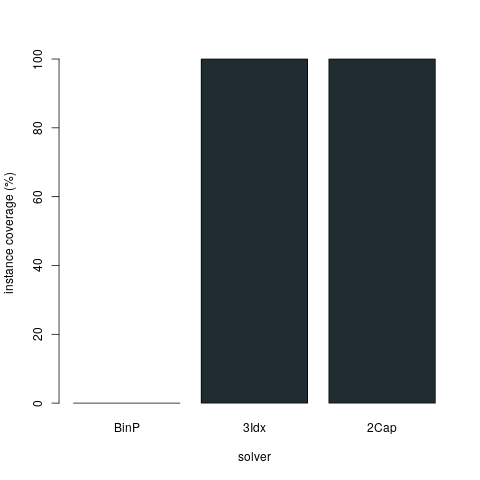
\includegraphics[width=1.2\textwidth]{img/solver_instance_coverage_b=2_s_1s.png}
\caption{\textsc{Zeitlimit 1s}}
\label{fig:instance_cov_b=2_s_a}
\end{subfigure}
\hfill
\begin{subfigure}[b]{0.3\textwidth}
\centering
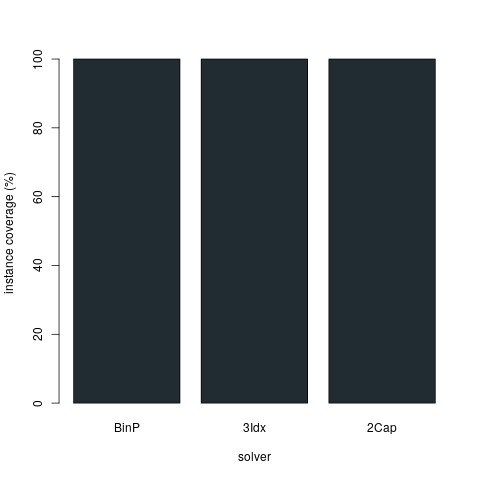
\includegraphics[width=1.2\textwidth]{img/solver_instance_coverage_b=2_s_3s.png}
\caption{\textsc{Zeitlimit 3s}}
\label{fig:instance_cov_b=2_s_b}
\end{subfigure}
\hfill
\begin{subfigure}[b]{0.3\textwidth}
\centering
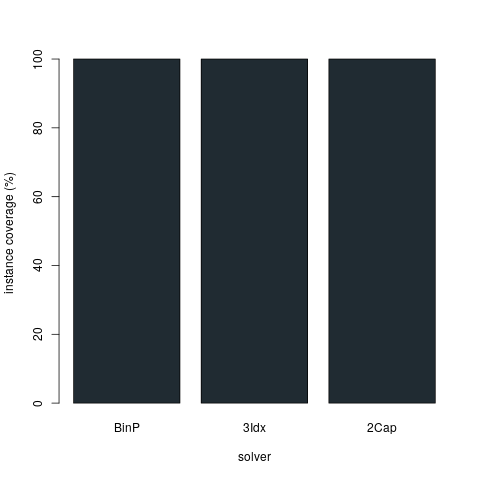
\includegraphics[width=1.2\textwidth]{img/solver_instance_coverage_b=2_s_5s.png}
\caption{\textsc{Zeitlimit 5s}}
\label{fig:instance_cov_b=2_s_c}
\end{subfigure}

\caption{\textsc{Instance-Coverage der $b=2$ Solver (s)}}
\label{fig:instance_cov_b=2_s}
\end{figure}

\pagebreak

In Abb. \ref{fig:b=2_s_runtimes} sind die Laufzeiten der Solver pro Instanz in Sekunden bei einem Zeitlimit von $5s$ dargestellt.
Man erkennt, dass die 3-Index-Formulierung deutlich schneller ist als die Bin-Packing-Formulierung und, dass die Heuristik beide MIP-Formulierungen noch einmal deutlich unterbietet. Da in der Abb. nur die absoluten Laufzeitdifferenzen zu sehen sind,
ist es wichtig, zu erwähnen, dass die Laufzeiten der Heuristik durchschnittlich um den Faktor $55.0$ kleiner sind,
als die der 3-Index-Formulierung. Zwischen der 3-Index- und der Bin-Packing-Formulierung liegt dagegen nur ein Faktor von $2.7$.

Aufgrund der Tatsache, dass CPLEX nur dann vor dem Zeitlimit terminiert, wenn die Instanz optimal gelöst wurde, ist klar
ersichtlich, dass die 3-Index-Formulierung sämtliche Instanzen nach etwa $1s$ optimal löst während die Bin-Packing-Formulierung in wenigen Fällen durch das Zeitlimit gestoppt wird.\newline
Bei den Instanzen $01$ und $08$, bei denen die Bin-Packing-Formulierung durch das Zeitlimit gestoppt wurde und dementsprechend nicht
notwendigerweise eine optimale Lösung gefunden hat, konnte die Heuristik, wie man Abb. \ref{fig:b=2_s_costs} entnehmen kann, sogar
bessere Zielfunktionswerte erzielen, als die Bin-Packing-Formulierung.\newline
Die weiteren Zielfunktionswerte der Bin-Packing-Formulierung sind in Abb. \ref{fig:b=2_s_costs}  deshalb nicht zu erkennen,
weil sie durch die Zielfunktionswerte der 3-Index-Formulierung verdeckt werden. Da beide Formulierungen die entsprechenden
Instanzen optimal lösen, kommen sie jeweils zum selben Zielfunktionswert.

\begin{figure}[H]
\centering
\begin{subfigure}[b]{0.4\textwidth}
\centering
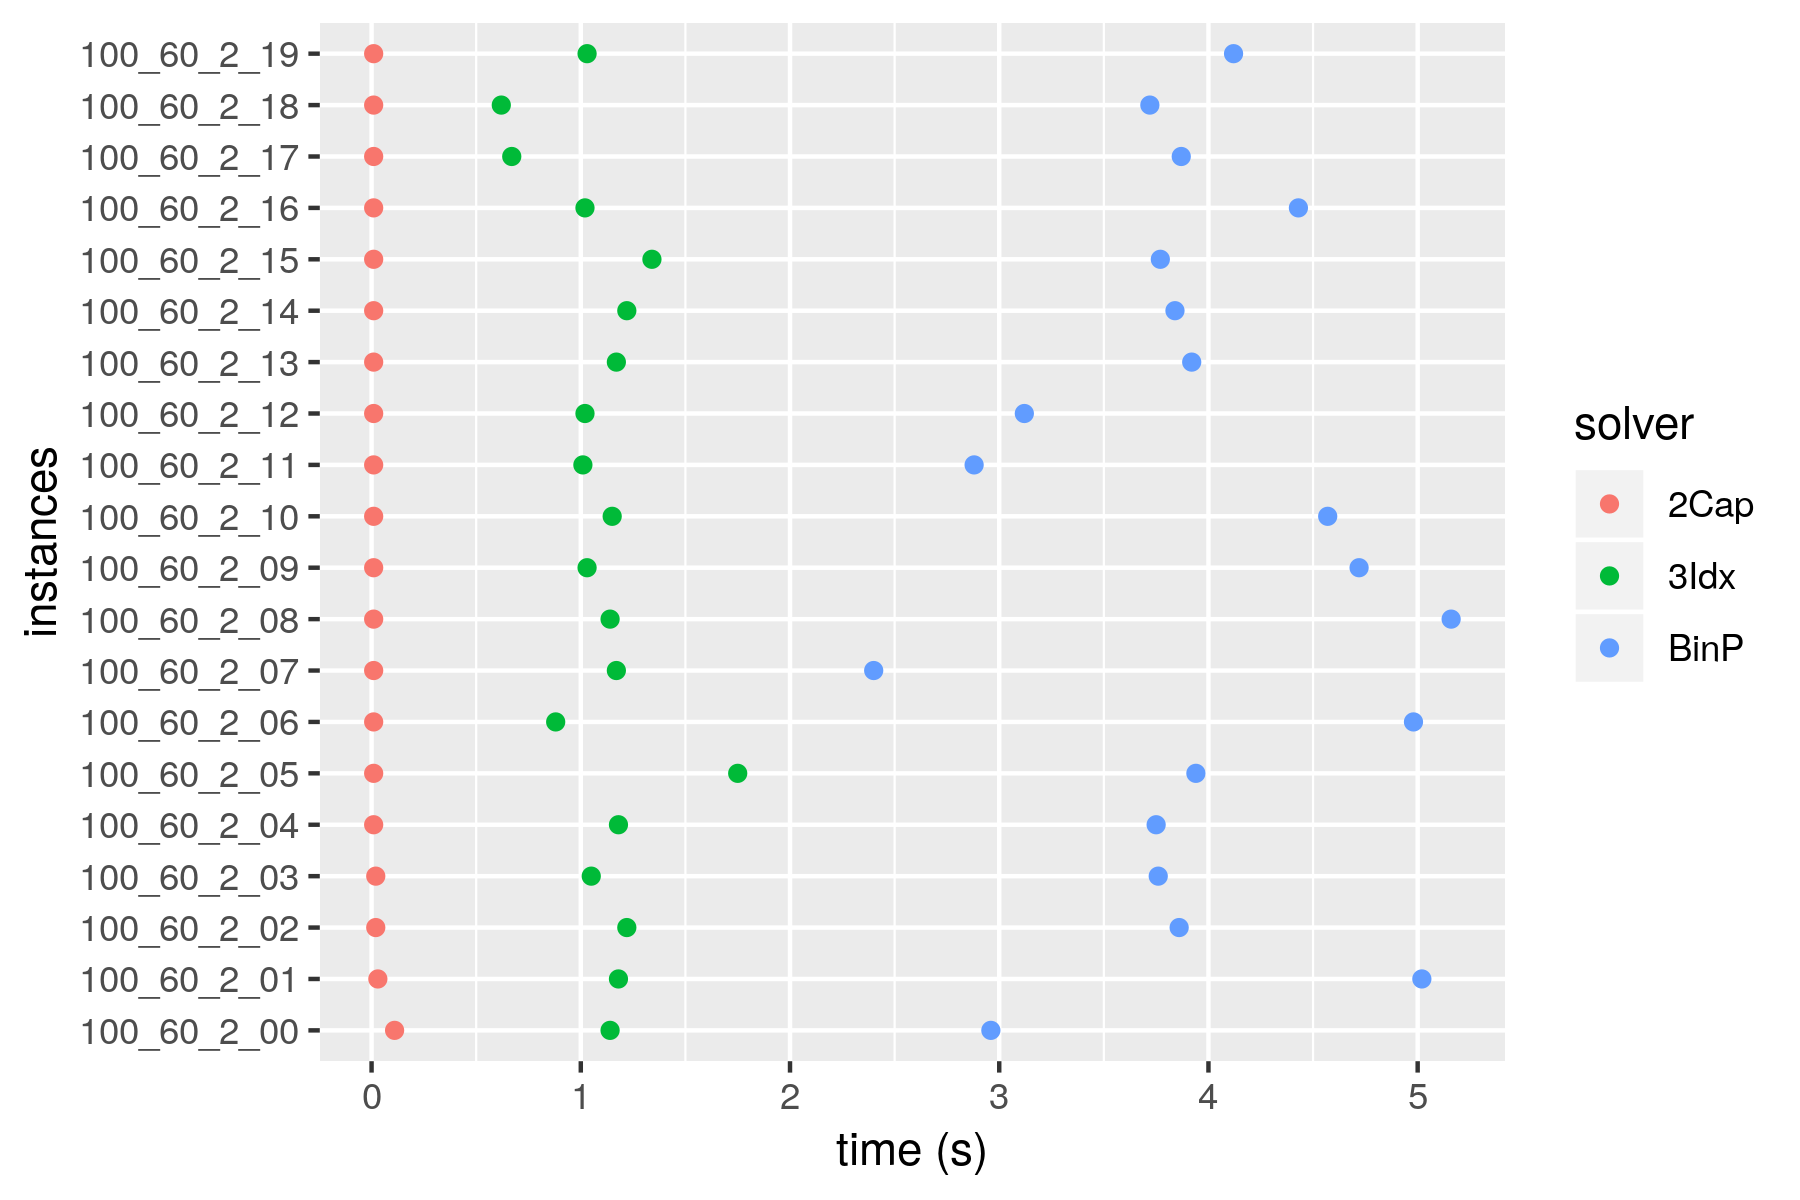
\includegraphics[width=1.3\textwidth]{img/solver_instance_time_b=2_s_5s.png}
\caption{\textsc{Laufzeiten bei 5s Zeitlimit}}
\label{fig:b=2_s_runtimes}
\end{subfigure}
\hfill
\begin{subfigure}[b]{0.4\textwidth}
\centering
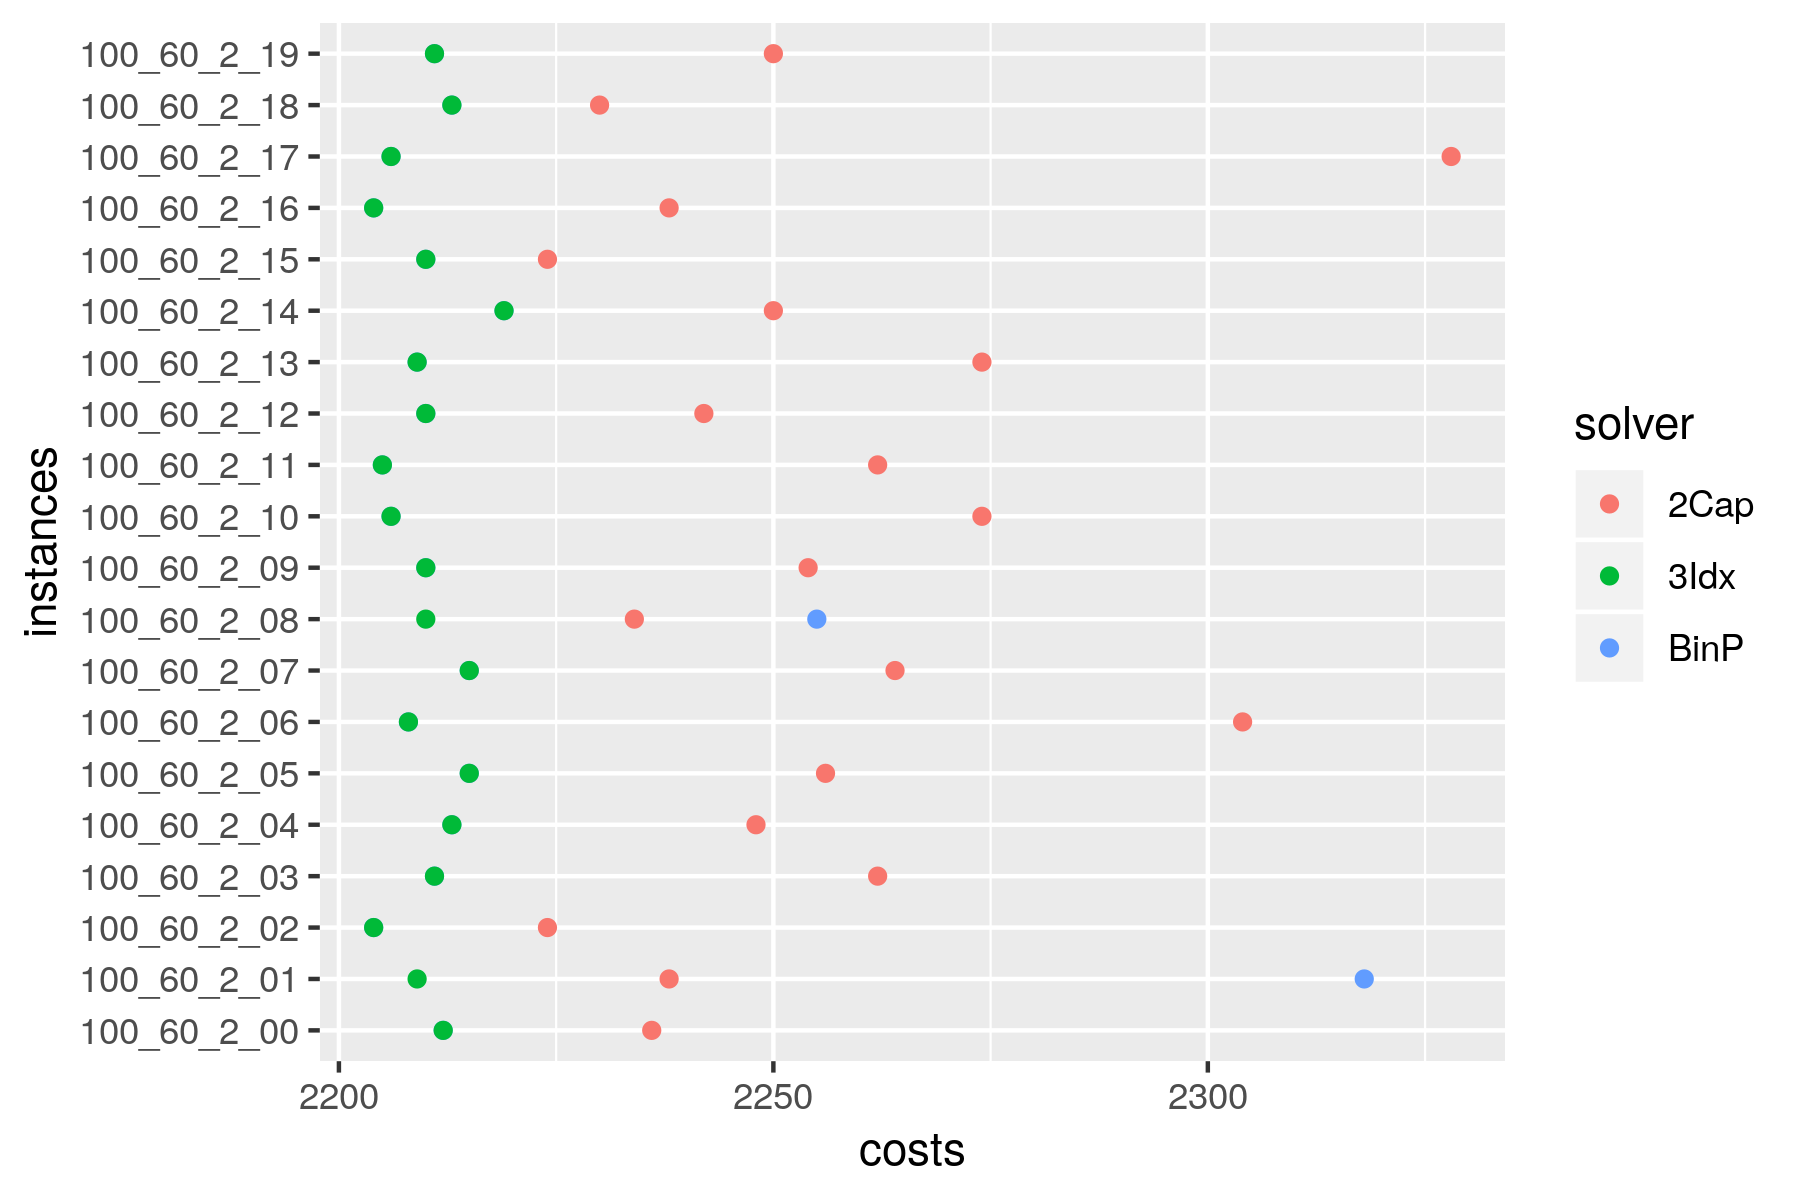
\includegraphics[width=1.3\textwidth]{img/solver_instance_cost_b=2_s_5s.png}
\caption{\textsc{Kosten bei 5s Zeitlimit}}
\label{fig:b=2_s_costs}
\end{subfigure}
\caption{}
\end{figure}

Die exakten Ergebnisse der MIP-Formulierungen sind den Tabellen in Abb. \ref{fig:table} zu entnehmen.
\textquote{Optimal} bezeichnet den prozentualen Anteil der Instanzen, die optimal gelöst wurden. Bei der \textquote{Laufzeit} handelt
es sich um die durchschnittliche Laufzeit pro Instanz in Sekunden und \textquote{Abweichung} gibt die durchschnittliche prozentuale Abweichung
vom Optimum pro Instanz an.

\begin{figure}[H]
\centering

\begin{subfigure}[b]{0.3\textwidth}
\centering
\resizebox{\textwidth}{!}{
\begin{tabular}{ | l | l | l |}
    \hline
     & \textbf{BinP} & \textbf{3Idx} \\ \hline
    \textbf{Optimal} & $ \textcolor{red}{0 \%}$ & $ \textcolor{mygreen}{35 \%}$ \\ \hline
    \textbf{Laufzeit} & $\textcolor{red}{---}$ & \O $\thinspace \textcolor{mygreen}{0.9 s}$ \\ \hline
    \textbf{Abweichung} & $\textcolor{red}{---}$ & \O $\thinspace \textcolor{mygreen}{2.0 \%}$ \\ \hline
\end{tabular}}
\caption{\textsc{Zeitlimit} $1s$}
\label{fig:res_b=2_s_a}
\end{subfigure}
% $\quad\quad\quad\quad$
\begin{subfigure}[b]{0.3\textwidth}
\centering
\resizebox{\textwidth}{!}{
\begin{tabular}{ | l | l | l |}
    \hline
     & \textbf{BinP} & \textbf{3Idx} \\ \hline
    \textbf{Optimal} & $ \textcolor{red}{10 \%}$ & $ \textcolor{mygreen}{100 \%}$ \\ \hline
    \textbf{Laufzeit} & \O $\thinspace \textcolor{red}{3.0 s}$ & \O $\thinspace \textcolor{mygreen}{1.1 s}$ \\ \hline
    \textbf{Abweichung} & \O $\thinspace \textcolor{red}{4.7 \%}$ & \O $\thinspace \textcolor{mygreen}{0.0 \%}$ \\ \hline
\end{tabular}}
\caption{\textsc{Zeitlimit} $3s$}
\label{fig:res_b=2_s_b}
\end{subfigure}
% \end{figure}
% \begin{figure}[H]
\begin{subfigure}[b]{0.3\textwidth}
\centering
\resizebox{\textwidth}{!}{
\begin{tabular}{ | l | l | l |}
    \hline
     & \textbf{BinP} & \textbf{3Idx} \\ \hline
    \textbf{Optimal} & $ \textcolor{red}{90 \%}$ & $ \textcolor{mygreen}{100 \%}$ \\ \hline
    \textbf{Laufzeit} & \O $\thinspace \textcolor{red}{3.9 s}$ & \O $\thinspace \textcolor{mygreen}{1.1 s}$ \\ \hline
    \textbf{Abweichung} & \O $\thinspace \textcolor{red}{0.4 \%}$ & \O $\thinspace \textcolor{mygreen}{0.0 \%}$ \\ \hline
\end{tabular}}
\caption{\textsc{Zeitlimit} $5s$}
\label{fig:res_b=2_s_c}
\end{subfigure}

\caption{\textsc{MIP-Ergebnisse}}
\label{fig:table}
\end{figure}

Abb. \ref{fig:table} zeigt, dass die 3-Index-Formulierung bei jedem betrachteten Zeitlimit eine geringere Laufzeit benötigt
als die Bin-Packing-Formulierung und somit zu besseren Ergebnissen kommt.

Da die Zeitlimits aufgrund der geringen Laufzeit für die Heuristik keine Rolle spielen, kommt diese stets zum selben Ergebnis.
Sie weicht durchschnittlich um $2.0 \%$ vom Optimum ab und benötigt dafür eine Laufzeit von nur $0.02s$.

Trotz dieser guten Ergebnisse der Heuristik, besteht aufgrund der Tatsache, dass die 3-Index-Formulierung sämtliche Instanzen
mit einer durchschnittlichen Laufzeit von $1.1s$ optimal löst, aus praktischer Perspektive vermutlich eher kein großer Bedarf für
eine Laufzeitverbesserung durch eine Heuristik.

\textbf{Mittelgroße Instanzen (m)}

Interessanter wird es bereits beim Vergleich der Solver für in Kapitel \ref{sec:instance_sizes} als mittelgroß bezeichnete Instanzen,
bei denen es darum geht, $300$ eintreffende Items in die Storage-Area zu verladen.
In Abb. \ref{fig:instance_cov_b=2} ist erneut die Instance-Coverage der einzelnen Solver dargestelllt.

In Abb. \ref{fig:instance_cov_b=2_m_a} sieht man, dass die Bin-Packing-Formulierung nach einer Minute noch keine Instanz gelöst hat, während die
3-Index-Formulierung dort bereits $80 \%$ der Instanzen löst. Selbst bei einem Zeitlimit von $10$ Minuten pro Instanz löst die Bin-Packing-Formulierung nur $20 \%$ der Instanzen, 3-Index löst bei diesem Zeitlimit sämtliche Instanzen
(vgl. Abb. \ref{fig:instance_cov_b=2_m_b}).
Bei einem Zeitlimit von $20$ Minuten löst schließlich auch die Bin-Packing-Formulierung sämtliche Instanzen
(vgl. Abb. \ref{fig:instance_cov_b=2_m_c}). Die Heuristik löst, wie bereits in der Kategorie der kleinen Instanzen,
in jedem Fall sämtliche Instanzen.
\begin{figure}[H]
\centering

\begin{subfigure}[b]{0.3\textwidth}
\centering
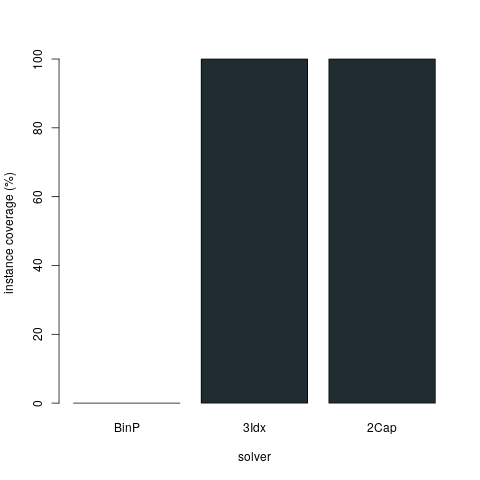
\includegraphics[width=1.2\textwidth]{img/solver_instance_coverage_b=2_m_60s.png}
\caption{\textsc{Zeitlimit} $1min$}
\label{fig:instance_cov_b=2_m_a}
\end{subfigure}
\hfill
\begin{subfigure}[b]{0.3\textwidth}
\centering
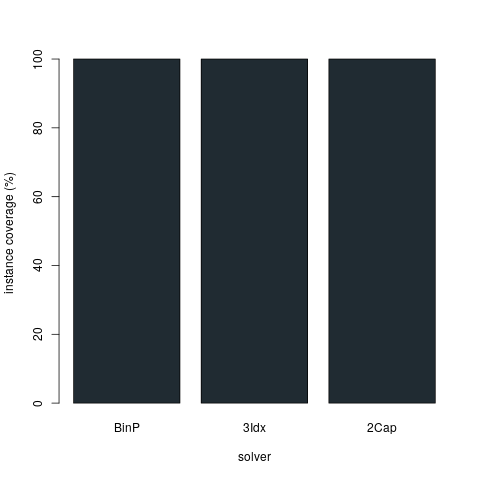
\includegraphics[width=1.2\textwidth]{img/solver_instance_coverage_b=2_m_600s.png}
\caption{\textsc{Zeitlimit} $10min$}
\label{fig:instance_cov_b=2_m_b}
\end{subfigure}
\hfill
\begin{subfigure}[b]{0.3\textwidth}
\centering
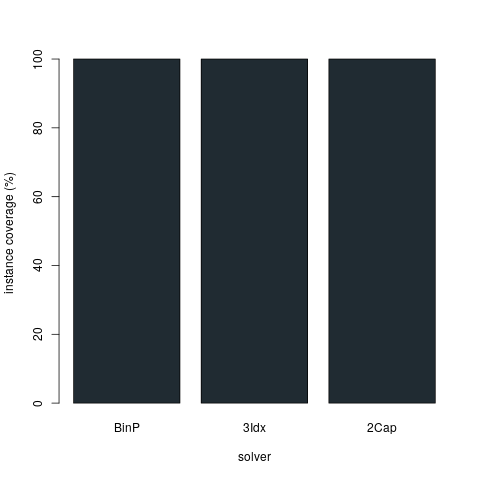
\includegraphics[width=1.2\textwidth]{img/solver_instance_coverage_b=2_m_1200s.png}
\caption{\textsc{Zeitlimit} $20min$}
\label{fig:instance_cov_b=2_m_c}
\end{subfigure}
\caption{\textsc{Instance-Coverage der $b=2$ Solver (m)}}
\label{fig:instance_cov_b=2}
\end{figure}

Da die Zeitlimits aufgrund der geringen Laufzeit der Heuristik für diese erneut keine Rolle spielen,
kommt sie stets zum selben Ergebnis. Sie weicht durchschnittlich um $0.8 \%$ vom
Optimum ab und benötigt dafür eine Laufzeit von $0.1s$.

\pagebreak

In Abb. \ref{fig:res_plots_b=2_m} sind die Laufzeiten und ermittelten Zielfunktionswerte der Solver bei einem Zeitlimit von $20$
Minuten dargestellt. Da die Bin-Packing- und die 3-Index-Formulierung bei diesem Zeitlimit sämtliche Instanzen optimal lösen,
kommen sie stets zum selben Kostenwert (vgl. Abb \ref{fig:b=2_m_costs}),
wobei die Bin-Packing-Einträge in der Visualisierung erneut durch die Einträge der 3-Index-Formulierung verdeckt werden.
In Abb. \ref{fig:b=2_m_runtimes} ist gut zu erkennen, dass die Bin-Packing-Formulierung deutlich längere Laufzeiten als die 3-Index-Formulierung
und die Heurisktik benötigt, wobei die Heuristik noch einmal deutlich schneller ist. Dabei handelt es sich allerdings um die absoluten Laufeiten.
Im Wesentlichen ist der Laufzeitunterschied zwischen der Heuristik und der 3-Index-Formulierung deutlich größer, als der zwischen den beiden
MIP-Formulierungen. Zwischen der Heuristik, die durchschnittlich $0.1s$ benötigt und der 3-Index-Formulierung, die durchschnittlich $107.8s$ benötigt (vgl. Abb. \ref{fig:res_b=2_m_c}), besteht ein Faktor von $1077.0$ während zwischen den beiden MIP-Formulierungen nur ein Faktor von
$7.1$ besteht. Die absolute Darstellung ist in diesem Fall also etwas irreführend, da die Heuristik deutlich schneller ist als beide MIP-Formulierungen. Trotzdem würde man in diesem Fall aus praktischer Perspektive die 3-Index-Formulierung klar der Bin-Packing-Formulierung vorziehen, dieser Sachverhalt ist in Abb. \ref{fig:b=2_m_runtimes} gut dargestellt.

\begin{figure}[H]
\centering
\begin{subfigure}[b]{0.4\textwidth}
\centering
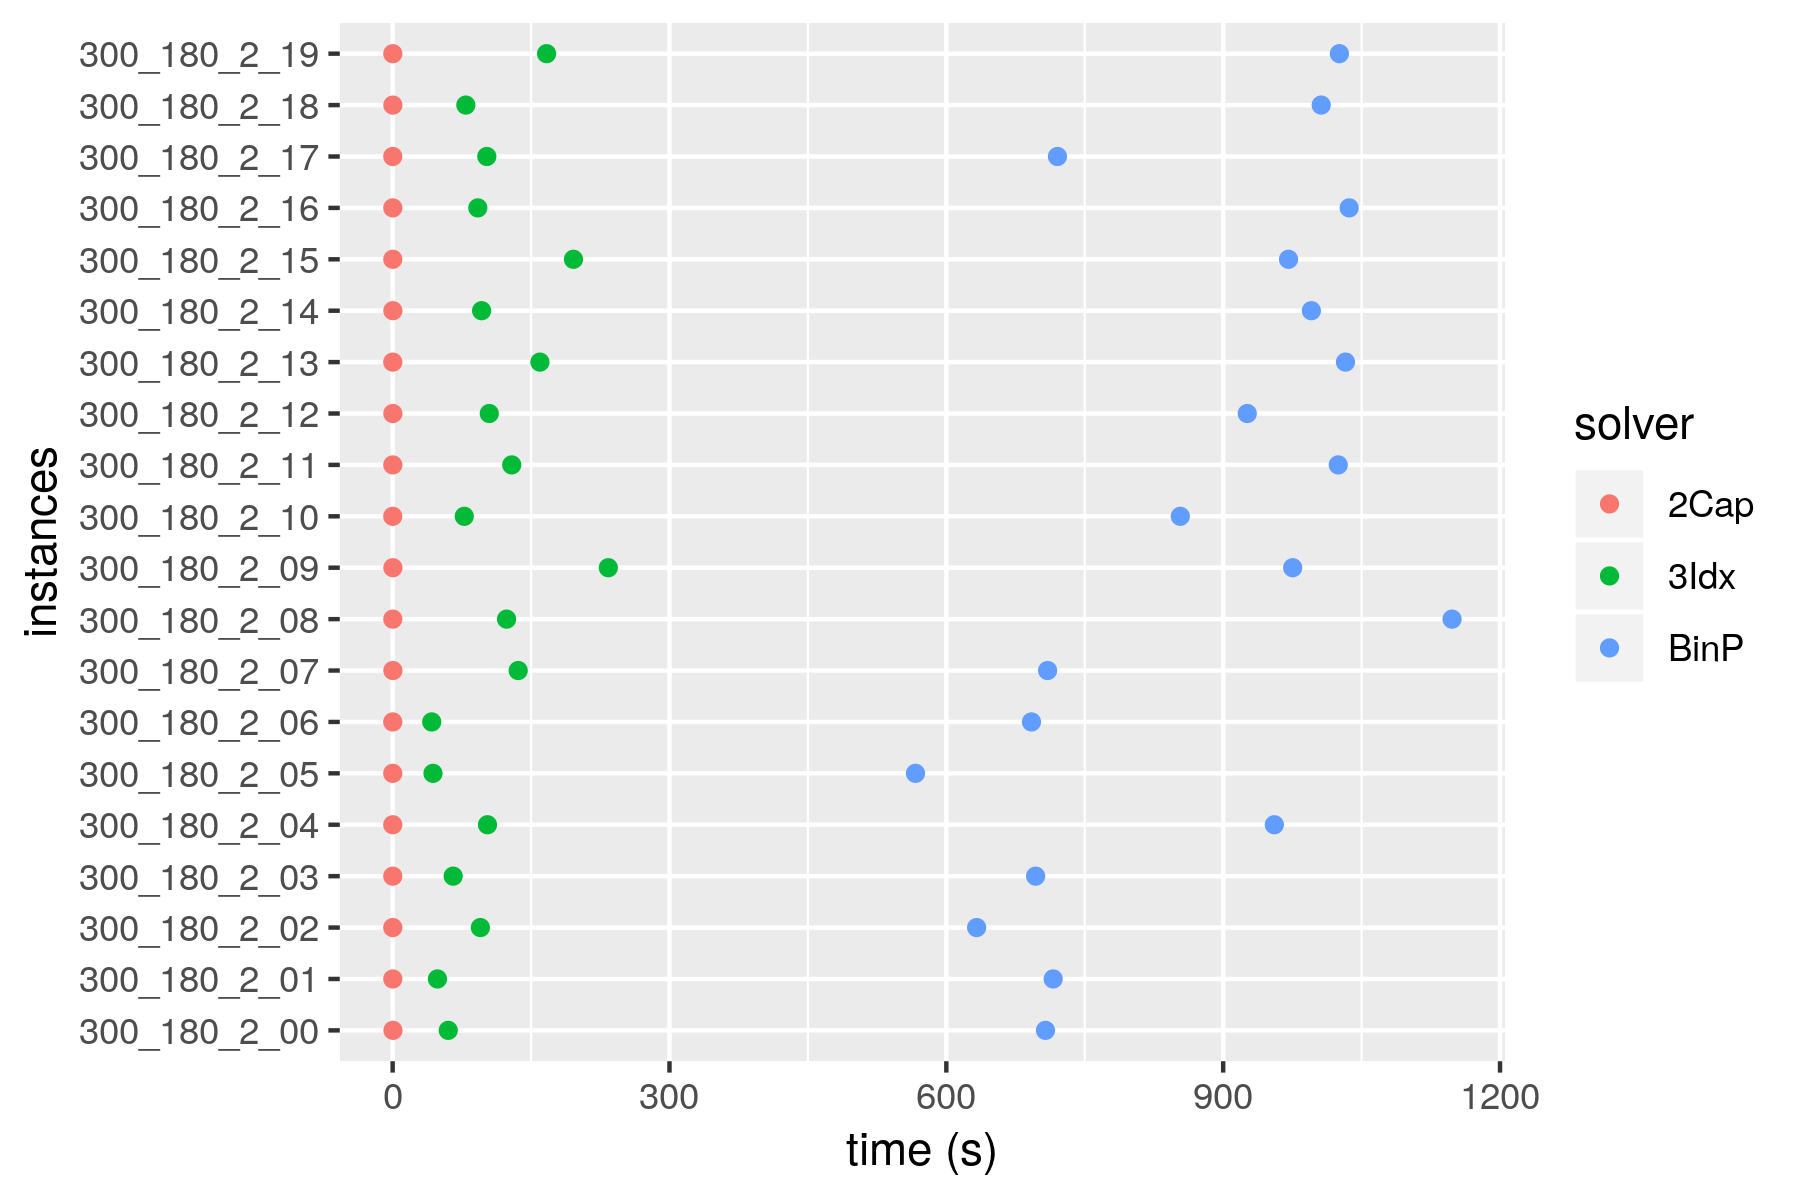
\includegraphics[width=1.3\textwidth]{img/solver_instance_time_b=2_m_1200s.png}
\caption{\textsc{Laufzeiten bei $20min$ Limit}}
\label{fig:b=2_m_runtimes}
\end{subfigure}
\hfill
\begin{subfigure}[b]{0.4\textwidth}
\centering
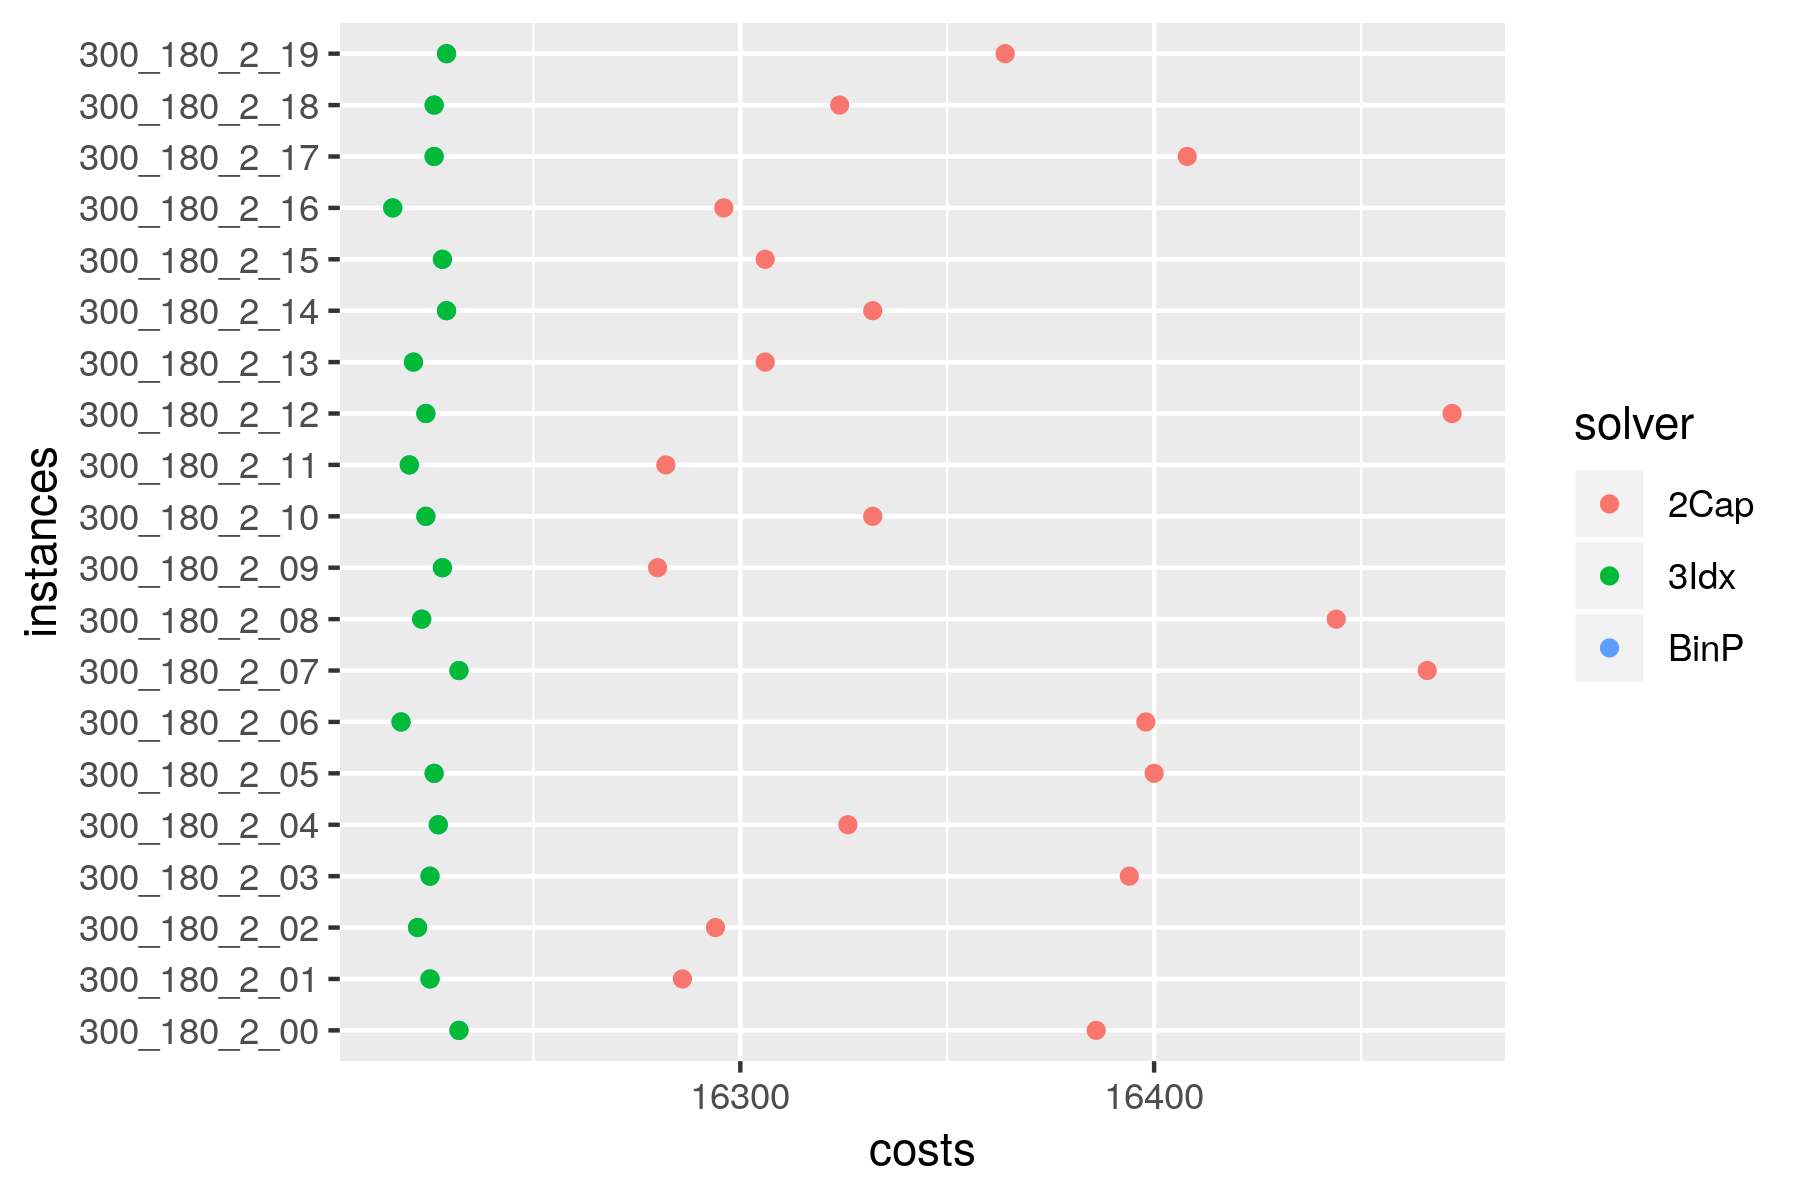
\includegraphics[width=1.3\textwidth]{img/solver_instance_cost_b=2_m_1200s.png}
\caption{\textsc{Kosten bei $20min$ Limit}}
\label{fig:b=2_m_costs}
\end{subfigure}
\caption{}
\label{fig:res_plots_b=2_m}
\end{figure}

In den Tabellen in Abb. \ref{fig:res_b=2_m} können die exakten Ergebnisse der MIP-Formulierungen nachvollzogen werden.
Wie bereits erwähnt, hat die Bin-Packing-Formulierung bei einem Zeitlimit von einer Minute keine Instanz gelöst, die 3-Index-Formulierung löst
$80 \%$ der Instanzen, allerdings nur $50 \%$ optimal (vgl. \ref{fig:res_b=2_m_a}). Die 3-Index-Formulierung benötigt dafür durchschnittlich
$55.4s$ und weicht, genau wie die Heuristik, um durchschnittlich $0.8 \%$ vom Optimum ab. Die Heuristik löst dabei allerdings sämtliche Instanzen
und benötigt nur durchschnittlich $0.1s$.

\begin{figure}[H]
% \end{figure}
% \begin{figure}[H]
% $\quad\quad\quad\quad$
\begin{subfigure}[b]{0.3\textwidth}
\centering
\resizebox{\textwidth}{!}{
\begin{tabular}{ | l | l | l |}
    \hline
     & \textbf{BinP} & \textbf{3Idx} \\ \hline
    \textbf{Optimal} & $ \textcolor{red}{0 \%}$ & $ \textcolor{mygreen}{50 \%}$ \\ \hline
    \textbf{Laufzeit} & $\textcolor{red}{----}$ & \O $\thinspace \textcolor{mygreen}{55.4 s}$ \\ \hline
    \textbf{Abweichung} & $\textcolor{red}{----}$ & \O $\thinspace \textcolor{mygreen}{0.8 \%}$ \\ \hline
\end{tabular}}
\caption{\textsc{Zeitlimit} $1min$}
\label{fig:res_b=2_m_a}
\end{subfigure}
\begin{subfigure}[b]{0.3\textwidth}
\centering
\resizebox{\textwidth}{!}{
\begin{tabular}{ | l | l | l |}
    \hline
     & \textbf{BinP} & \textbf{3Idx} \\ \hline
    \textbf{Optimal} & $ \textcolor{red}{10 \%}$ & $ \textcolor{mygreen}{100 \%}$ \\ \hline
    \textbf{Laufzeit} & \O $\thinspace \textcolor{red}{581.6 s}$ & \O $\thinspace \textcolor{mygreen}{73.7 s}$ \\ \hline
    \textbf{Abweichung} & \O $\thinspace \textcolor{red}{0.6 \%}$ & \O $\thinspace \textcolor{mygreen}{0.0 \%}$ \\ \hline
\end{tabular}}
\caption{\textsc{Zeitlimit} $10min$}
\label{fig:res_b=2_m_b}
\end{subfigure}
% \end{figure}
% \begin{figure}[H]
\begin{subfigure}[b]{0.3\textwidth}
\centering
\resizebox{\textwidth}{!}{
\begin{tabular}{ | l | l | l |}
    \hline
     & \textbf{BinP} & \textbf{3Idx} \\ \hline
    \textbf{Optimal} & $ 100 \%$ & $ 100 \%$ \\ \hline
    \textbf{Laufzeit} & \O $\thinspace 869.6 s$ & \O $\thinspace \textcolor{mygreen}{107.8 s}$ \\ \hline
    \textbf{Abweichung} & \O $\thinspace 0.0 \%$ & \O $\thinspace 0.0 \%$ \\ \hline
\end{tabular}}
\caption{\textsc{Zeitlimit} $20min$}
\label{fig:res_b=2_m_c}
\end{subfigure}
\caption{\textsc{MIP-Ergebnisse}}
\label{fig:res_b=2_m}
\end{figure}

Zusammenfassend ist die 3-Index-Formulierung in der Kategorie der mittelgroßen Instanzen der Bin-Packing-Formulierung vorzuziehen,
da sie bei allen betrachteten Zeitlimits die besseren Ergebnisse erzielt und auch bei einem Zeitlimit von $20$ Minuten, bei dem schließlich auch die Bin-Packing-Formulierung sämtliche Instanzen optimal löst, deutlich schneller ist als diese.

Die zu bevorzugende MIP-Formulierung 3-Index, benötigt, wie sich Abb. \ref{fig:res_b=2_m_b} entnehmen lässt, durchschnittlich
$73.7s$ um sämtliche Instanzen optimal zu lösen. Die Heuristik dagegen benötigt durchschnittlich $0.1s$ um sämtliche Instanzen
mit einer durchschnittlichen Abweichung vom Optimum von $0.8 \%$ zu lösen.

Dieser Laufzeitunterschied ist so erheblich, dass die gerine Abweichung vom Optimum in der Praxis vermutlich in Kauf genommen werden kann,
wenn sich damit eine derart große Laufzeitersparnis ergibt. In dieser Kategorie präsentiert sich die Heuristik also als sehr gute Alternative.

\textbf{Große Instanzen (l)}

Zuletzt werden die Solver für die in Kapitel \ref{sec:instance_sizes} als groß bezeichneten Instanzen, bei denen es darum geht,
$500$ eintreffende Items in die Storage-Area zu verladen, verglichen. In dieser Kategorie wurden noch einmal größere Zeitlimits von
$15$, $30$ und $45$ Minuten betrachtet.

In Abb. \ref{fig:instance_cov_b=2_l} ist die Instance-Coverage der Solver für die jeweiligen Zeitlimits dargestellt und es fällt auf,
dass die Bin-Packing-Formulierung überhaupt keine Instanz löst. Dies liegt zum einen daran, dass im jeweils betrachteten Zeitlimit
tatsächlich noch keine Lösung gefunden wurde, zum anderen aber auch daran, dass der Speicherbedarf den zur Verfügung stehenden Speicher
übersteigt. TODO: Grund checken: B\&B Tree?

\begin{figure}[H]
\centering

\begin{subfigure}[b]{0.3\textwidth}
\centering
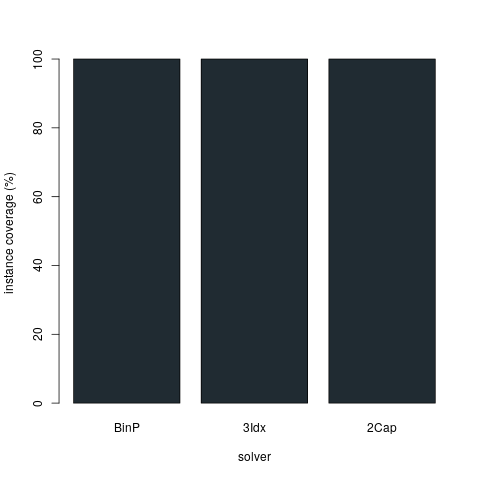
\includegraphics[width=1.2\textwidth]{img/solver_instance_coverage_b=2_l_900s.png}
\caption{\textsc{Zeitlimit} $15min$}
\label{fig:instance_cov_b=2_l_a}
\end{subfigure}
\hfill
\begin{subfigure}[b]{0.3\textwidth}
\centering
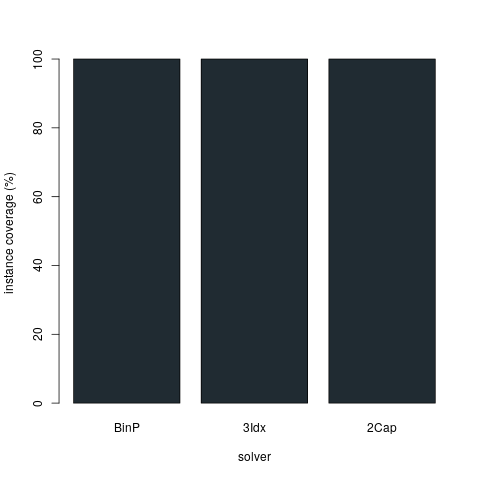
\includegraphics[width=1.2\textwidth]{img/solver_instance_coverage_b=2_l_1800s.png}
\caption{\textsc{Zeitlimit} $30min$}
\label{fig:instance_cov_b=2_l_b}
\end{subfigure}
\hfill
\begin{subfigure}[b]{0.3\textwidth}
\centering
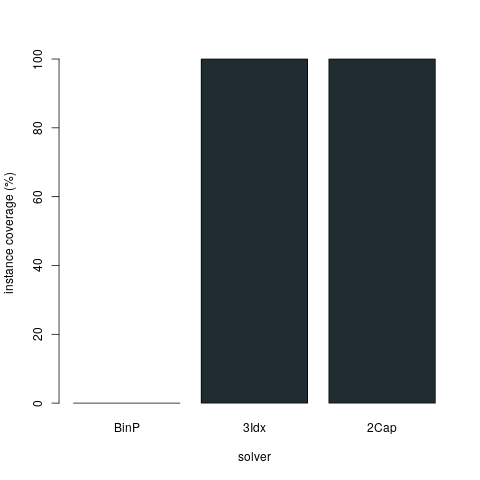
\includegraphics[width=1.2\textwidth]{img/solver_instance_coverage_b=2_l_2700s.png}
\caption{\textsc{Zeitlimit} $45min$}
\label{fig:instance_cov_b=2_l_c}
\end{subfigure}

\caption{\textsc{Instance-Coverage der $b=2$ Solver (l)}}
\label{fig:instance_cov_b=2_l}
\end{figure}

Überdies ist Abb. \ref{fig:instance_cov_b=2_l} zu enthnehmen, dass die 3-Index-Formulierung erst beim betrachteten
Zeitlimit von $45$ Minuten sämtliche Instanzen gelöst hat. Für die Heuristik sind die Zeitlimits erneut irrelevant,
da sie mit einer durchschnittlichen Laufzeit von $0.7s$ pro Instanz sämtliche Instanzen löst.

In Abb. \ref{fig:res_plots_b=2_l} bestätigt sich die Tendenz aus der Darstellung der Instance-Coverage.
Die Heuristik ist deutlich schneller als die 3-Index-Formulierung (vgl. Abb \ref{fig:b=2_l_runtimes}) und weicht dabei nur
unwesentlich vom optimalen Zielfunktionswert ab (vgl. \ref{fig:b=2_l_costs}).

\begin{figure}[H]
\centering
\begin{subfigure}[b]{0.4\textwidth}
\centering
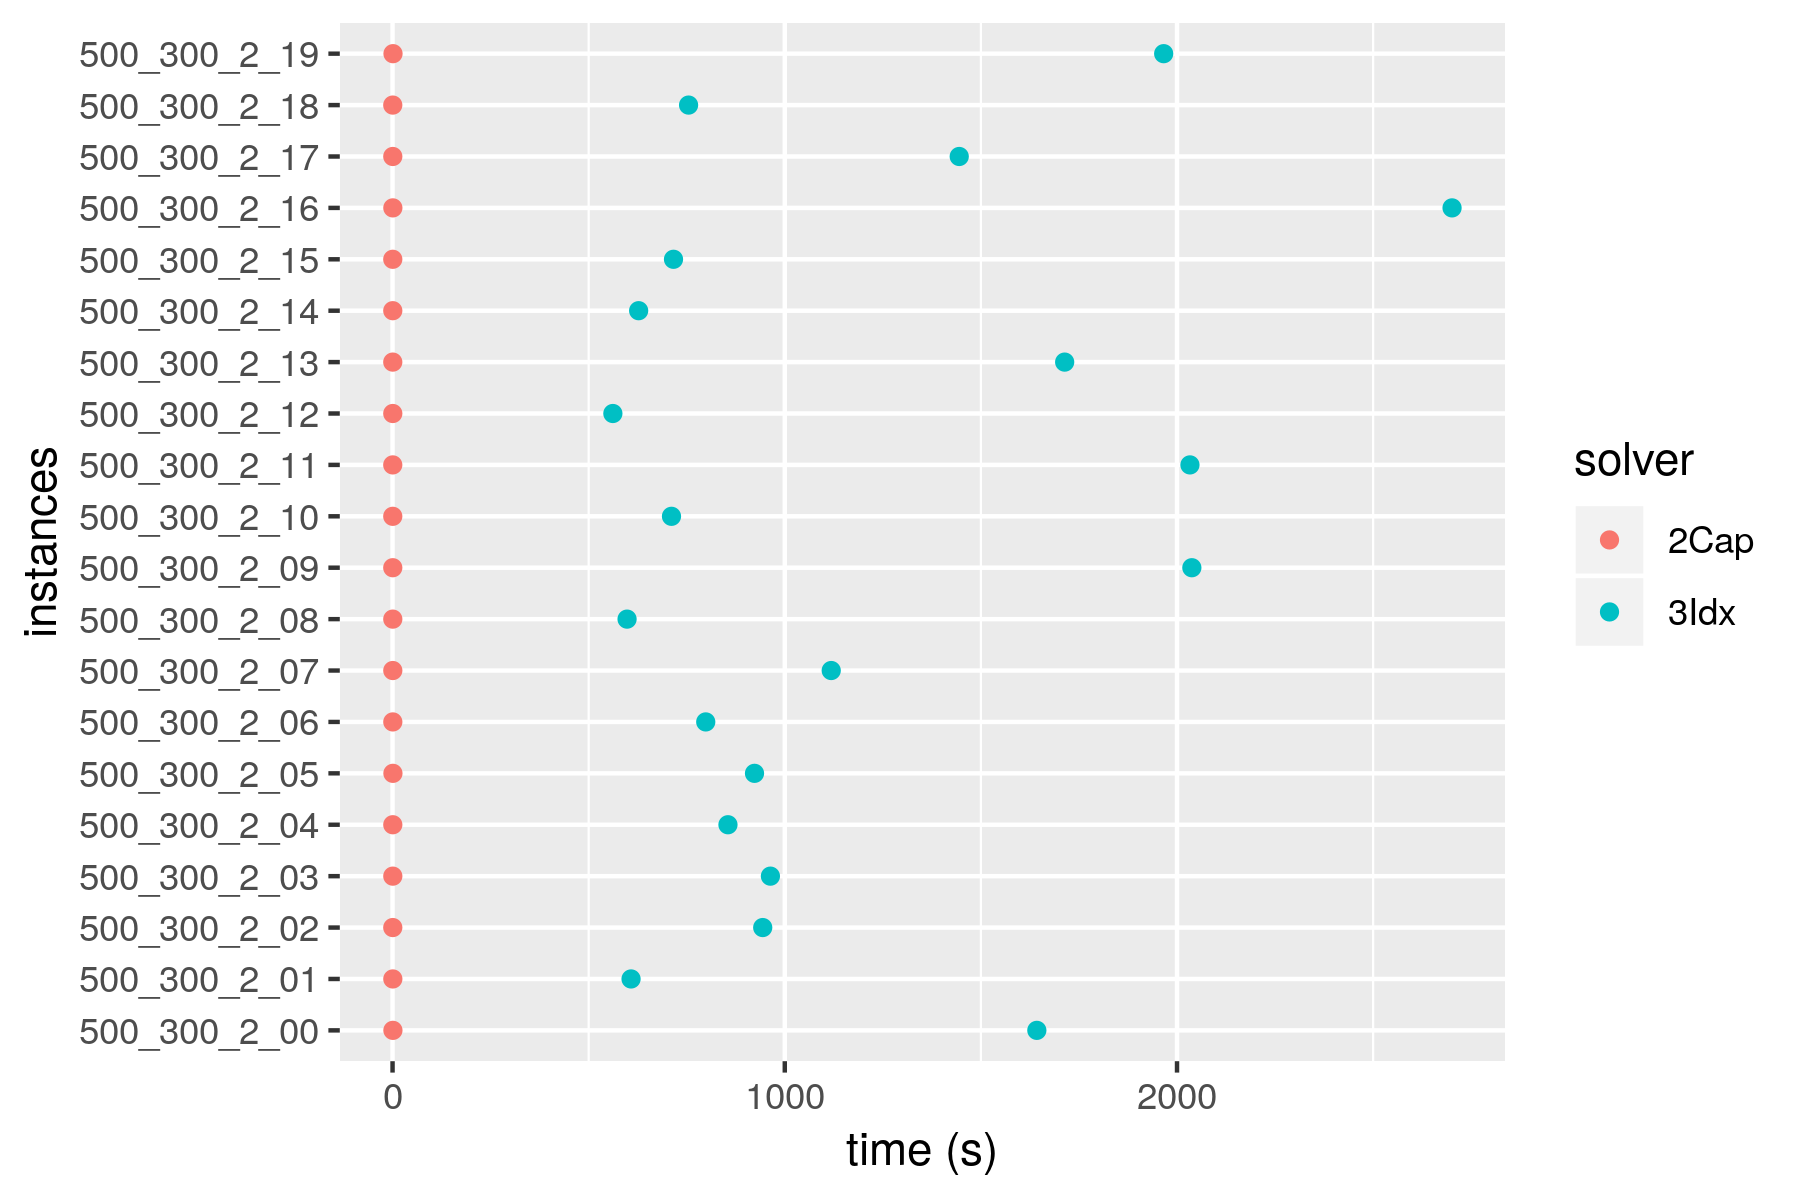
\includegraphics[width=1.3\textwidth]{img/solver_instance_time_b=2_l_2700s.png}
\caption{\textsc{Laufzeiten bei $45min$ Limit}}
\label{fig:b=2_l_runtimes}
\end{subfigure}
\hfill
\begin{subfigure}[b]{0.4\textwidth}
\centering
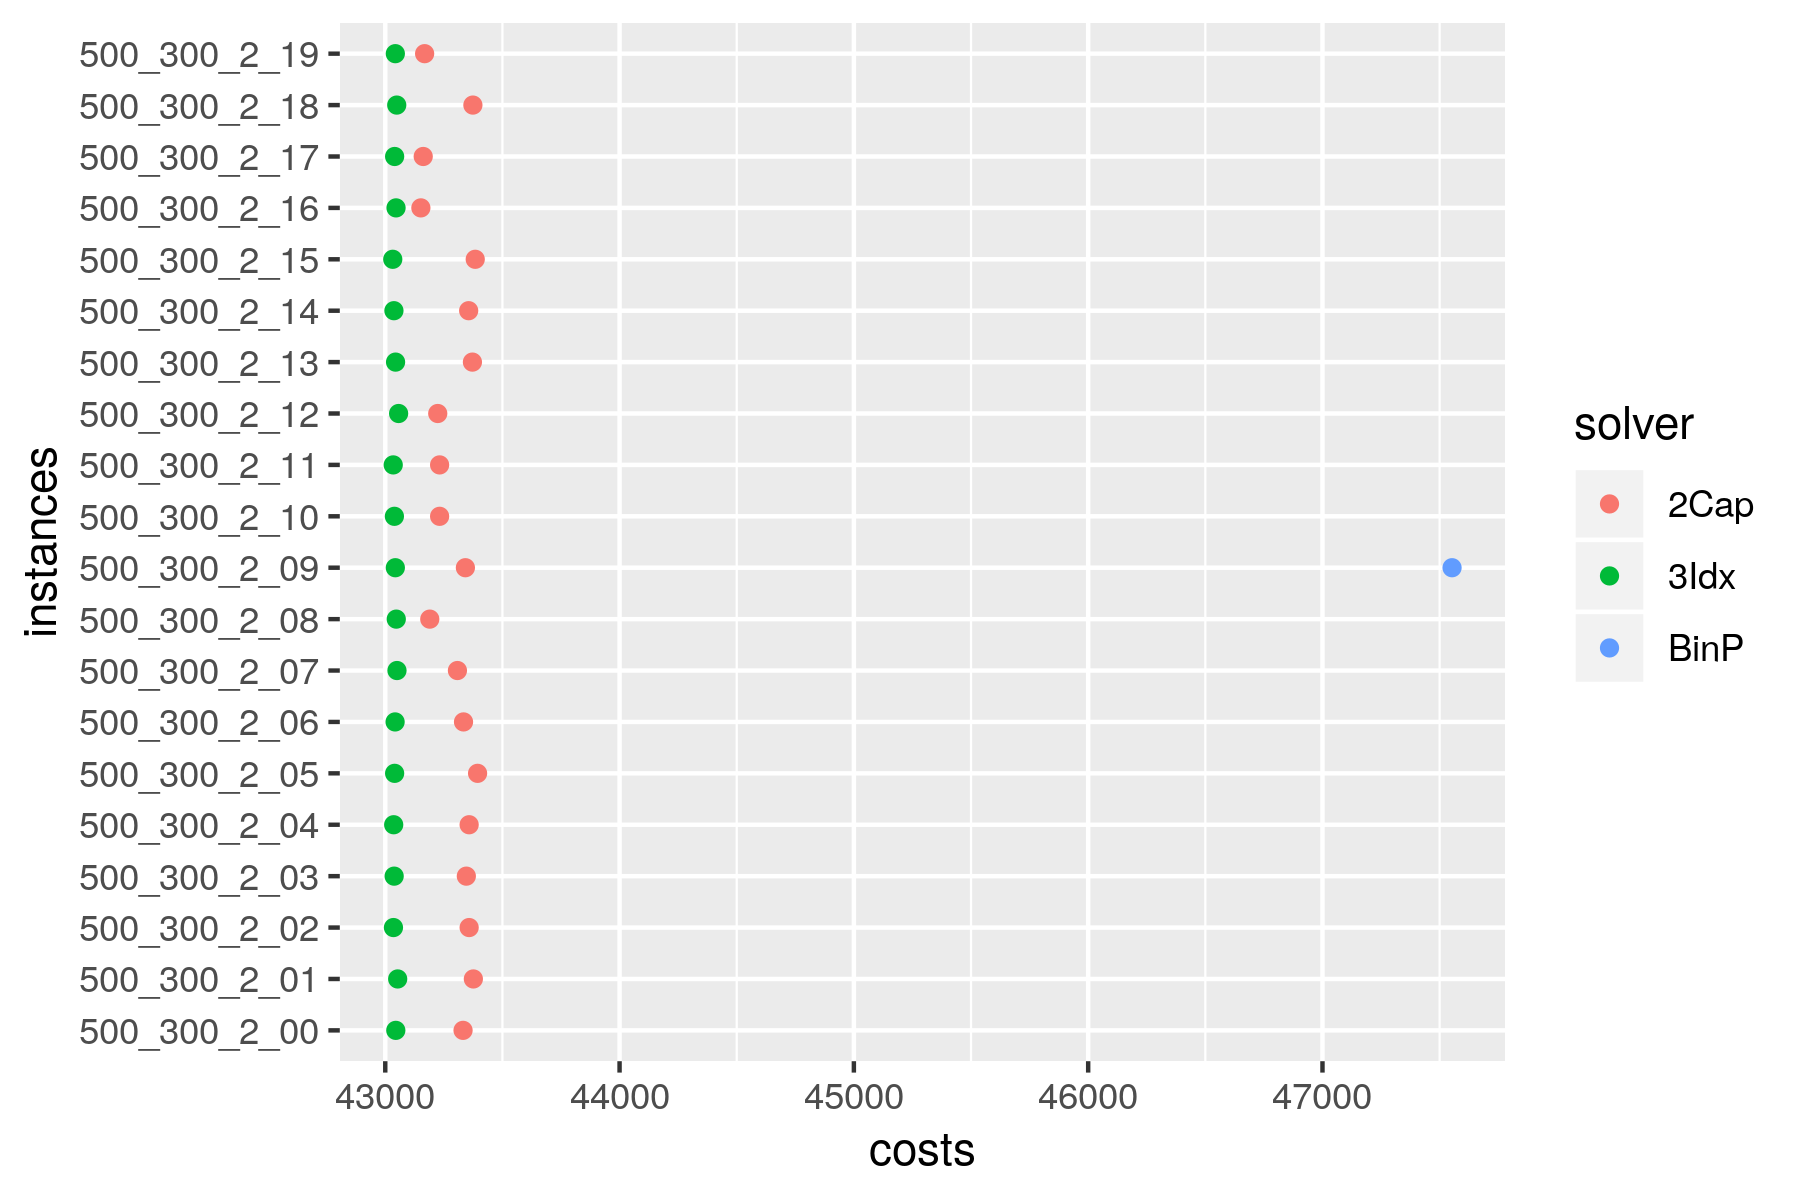
\includegraphics[width=1.3\textwidth]{img/solver_instance_cost_b=2_l_2700s.png}
\caption{\textsc{Kosten bei $45min$ Limit}}
\label{fig:b=2_l_costs}
\end{subfigure}
\caption{}
\label{fig:res_plots_b=2_l}
\end{figure}

In Abb. \ref{fig:res_b=2_l} sind die exakten Ergebnisse der MIP-Formulierungen aufgeführt, denen man
entnehmen kann, dass die 3-Index-Formulierung mit einer durchschnittlichen Laufzeit von ca. $20$ Minuten sämtliche Instanzen
optimal löst (vgl. Abb. \ref{fig:res_b=2_l_c}). Die Heuristik benötigt allerdings nur durchschnittlich $0.7s$ pro Instanz und
weicht auch nur um im Durchschnitt $0.6 \%$ vom Optimalwert ab. Dieser, verglichen mit der Kategorie der mittelgroßen Instanzen,
noch gravierende Laufzeitunterschied und die nur sehr geringe Abweichung vom Optimum sorgen dafür, dass die Heuristik in der Praxis,
wenn geringe Abweichungen gestattet sind, bevorzugt werden sollte.

\begin{figure}[H]
\begin{subfigure}[b]{0.3\textwidth}
\centering
\resizebox{\textwidth}{!}{
\begin{tabular}{ | l | l | l |}
    \hline
     & \textbf{BinP} & \textbf{3Idx} \\ \hline
    \textbf{Optimal} & $ \textcolor{red}{0 \%}$ & $ \textcolor{mygreen}{70 \%}$ \\ \hline
    \textbf{Laufzeit} & \textcolor{red}{$---$} & \O $\thinspace \textcolor{mygreen}{728.0 s}$ \\ \hline
    \textbf{Abweichung} & \textcolor{red}{$---$} & \O $\thinspace \textcolor{mygreen}{0.53 \%}$ \\ \hline
\end{tabular}}
\caption{\textsc{Zeitlimit} $15min$}
\label{fig:res_b=2_l_a}
\end{subfigure}
\begin{subfigure}[b]{0.3\textwidth}
\centering
\resizebox{\textwidth}{!}{
\begin{tabular}{ | l | l | l |}
    \hline
     & \textbf{BinP} & \textbf{3Idx} \\ \hline
    \textbf{Optimal} & $ \textcolor{red}{0 \%}$ & $ \textcolor{mygreen}{85 \%}$ \\ \hline
    \textbf{Laufzeit} & \textcolor{red}{$---$} & \O $\thinspace \textcolor{mygreen}{977.2 s}$ \\ \hline
    \textbf{Abweichung} & \textcolor{red}{$---$} & \O $\thinspace \textcolor{mygreen}{0.0 \%}$ \\ \hline
\end{tabular}}
\caption{\textsc{Zeitlimit} $30min$}
\label{fig:res_b=2_l_b}
\end{subfigure}
% $\quad\quad\quad\quad$
\begin{subfigure}[b]{0.3\textwidth}
\centering
\resizebox{\textwidth}{!}{
\begin{tabular}{ | l | l | l |}
    \hline
     & \textbf{BinP} & \textbf{3Idx} \\ \hline
    \textbf{Optimal} & $ \textcolor{red}{0 \%}$ & $ \textcolor{mygreen}{100 \%}$ \\ \hline
    \textbf{Laufzeit} & \textcolor{red}{$---$} & \O $\thinspace \textcolor{mygreen}{1185.9  s}$ \\ \hline
    \textbf{Abweichung} & \textcolor{red}{$---$} & \O $\thinspace \textcolor{mygreen}{0.0 \%}$ \\ \hline
\end{tabular}}
\caption{\textsc{Zeitlimit} $45min$}
\label{fig:res_b=2_l_c}
\end{subfigure}

\caption{\textsc{MIP-Ergebnisse}}
\label{fig:res_b=2_l}
\end{figure}

\textbf{Fazit}

Insgesamt ist festzuhalten, dass bei Stacking-Problemen mit Stacks der Kapazität $b = 2$ in der Kategorie der kleinen Instanzen
aufgrund der geringen Laufzeit der MIP-Formulierungen kein wirklicher Bedarf für eine Laufzeitverbesserung besteht.
Anders in den Kategorien der mittelgroßen und großen Instanzen, bei welchen die Heuristik bei nur kleinen Abweichungen zu einer
derart großen Laufzeiteinparung führt, dass sie eine für die Praxis relevante Alternative darstellt.

\subsection{Konstruktive Heuristik ($b = 3$)}
\label{sec:three_cap_heuristic}

In diesem Abschnitt wird die konstruktive Heuristik zur Lösung von Stacking-Problemen
mit Stacks der Kapazität $b = 3$ vorgestellt. Viele der Ansätze funktionieren analog zur Heuristik für $b = 2$
aus Kapitel \ref{sec:two_cap_heuristic}.

Zunächst wird, wie auch in der Heuristik für $b = 2$, ein Stacking-Constraint-Graph $G = (V, E)$ generiert, welcher die Items
als Knoten enthält, d.h. $V = I$. Dieser Graph enthält eine Kante $\{i, j\}$ zwischen zwei Knoten,
wenn die entsprechenden Items $i, j \in I$ in mindestens einer Richtung stackbar sind, d.h., wenn $s_{ij} + s_{ji} \geq 1$.

Nun wird, ebenfalls analog zur Heuristik aus \ref{sec:two_cap_heuristic}, ein \textsc{MCM} in $G$ berechnet,
dessen Kanten als Paare von Items intepretiert werden.
Da die Stacks nun jedoch nicht nur Paare, sondern Tripel von Items beinhalten können, wird im nächsten Schritt versucht,
eben solche Tripel von kompatiblen Items zu generieren. Dafür wird zunächst ein weiterer Graph $G_1$ eingeführt,
welcher die zuvor generierten Item-Paare und die verbleibenden Unmatched Items als Knoten enthält.
Dieser Graph besitzt eine Kante zwischen einem Item-Paar und einem Unmatched Item,
wenn diese kompatibel sind, d.h., wenn das Unmatched Item dem Paar zugeordnet werden kann und ein Tripel entsteht, welches
stapelbar ist, also die Stacking Constraints respektiert.

Anschließend wird in $G_1$ ein \textsc{MCM} berechnet, dessen Kanten einer größtmöglichen Menge an kompatiblen Item-Tripeln entspricht.
Die verbleibenden Item-Paare, für die kein passendes Unmatched Item gefunden wurde, werden nun in einem weiteren Schritt,
wenn möglich, zu Tripeln gemergt. (TODO: Merge-Step vorstellen).

Da im Zuge des Merge-Prozesses weitere Unmatched Items entstehen können und auch nicht notwendigerweise sämtliche vorherigen Unmatched Items
einem Paar zugeordnet wurden, werden nun abermals aus allen verbleibenden Items Paare gebildet, was erneut durch ein \textsc{MCM}
auf dem für diese Items generierten Stacking-Constraint-Graphen geschieht. Die dabei entstehenden Unmatched Items werden schließlich
im Folgenden auch als solche betrachtet.

An dieser Stelle liegt also eine Menge an Tripeln, eine Menge an Paaren und eine Menge an Unmatched Items vor. Diese müssen nun
noch in einer die Stacking Constraints respektierenden Weise den Stacks zugewiesen werden.

Zu diesem Zweck wird ein bipartiter Graph generiert, welcher die Items, bestehend aus Tripeln, Paaren und Unmatched Items, in der einen Partition
und die Stacks in der anderen Partition enthält. Dabei gibt es, wie schon bei der Heuristik für $b = 2$, initial eine Kante von jedem Tripel, Paar und Item zu jedem Stack. D.h. im Prinzip sind sämtliche Items mit jedem Stack kompatibel. Dies liegt daran, dass die Placement Constraints indirekt über hohe Kostenwerte implementiert wurden und nicht direkt durch ein Vermeiden der entsprechenden Kanten. Der Grund für diese Entscheidung wurde bereits in Kapitel \ref{sec:placement_restrictions} erläutert. Die inkompatiblen Item-Stack-Zuweisungen werden
also, sofern möglich, indirekt durch das \textsc{MWPM} ausgeschlossen.

\pagebreak

Im nächsten Schritt wird ebendieses \textsc{MWPM} im bipartiten Graphen berechnet, dessen Kanten
als Stack-Zuweisungen interpretiert werden. Zuletzt muss dann wiederum ggf. die Reihenfolge der Items innerhalb der Stacks so angepasst werden,
dass sie die Stacking Constraints respektieren. Dabei ist wieder garantiert, dass eines solche Sortierung möglich ist und trivial durch den
Algorithmus \ref{alg:algo1} erfolgen kann.\newline

\textbf{Beispiel}

Gegeben sei die Item-Menge $I = \{0, 1, 2, 3, 4, 5, 6, 7, 8, 9\}$ sowie eine Stack-Kapazität von $b = 3$. Die Anzahl der
zur Verfügung stehenden Stacks von $m = 4$ ergibt sich basierend auf der Beschreibung in Abschnitt \ref{sec:test_data}.

Zunächst wird der Stacking-Constraint-Graph für die Item-Menge $I$ generiert, auf welchem dann analog zum Beispiel aus Abschnitt
\ref{sec:two_cap_heuristic} ein \textsc{MCM} berechnet wird. In Abb. \ref{fig:pairs_and_unmatched} ist das Ergebnis dargestellt,
welches die Kanten des \textsc{MCM} interpretiert als Item-Paare in grün zeigt. Die als unmatched verbleibenden Items sind in rot dargestellt.

\begin{figure}[H]
\centering
\begin{tikzpicture}[scale=0.85, transform shape, node distance=2cm]
        \node[state] (A) [thick] {$\boldsymbol{\textcolor{mygreen}{0, 2}}$};
        \node[state] (B) [thick, right of=A] {$\boldsymbol{\textcolor{mygreen}{1, 9}}$};
        \node[state] (C) [thick, right of=B] {$\boldsymbol{\textcolor{mygreen}{3, 4}}$};
        \node[state] (D) [thick, right of=C] {$\boldsymbol{\textcolor{mygreen}{5, 6}}$};
        \node[state] (E) [thick, right of=D] {$\boldsymbol{\textcolor{red}{7}}$};
        \node[state] (F) [thick, right of=E] {$\boldsymbol{\textcolor{red}{8}}$};
        \path;
\end{tikzpicture}
\caption{\textsc{Item-Paare und Unmatched-Items.}}
\label{fig:pairs_and_unmatched}
\end{figure}

Anschließend wird der in Abb. \ref{fig:graph_for_pairs_and_unmatched} dargestellte Graph generiert, welcher die Paare und
Unmatched Items als Knoten enthält. Eine Kante zwischen einem Unmatched Item und einem Paar bedeutet, dass dieses Unmatched
Item dem Paar zugeordnet werden kann, sodass ein kompatibles Tripel entsteht.
In diesem Fall ist also lediglich die $7$ kompatibel zu zwei Paaren, zu $(3, 4)$ und zu $(5, 6)$.

\begin{figure}[H]
\centering
\begin{tikzpicture}[scale=0.85, transform shape, node distance=2cm]
        \node[state] (A) [thick] {$\boldsymbol{0, 2}$};
        \node[state] (B) [thick, right of=A] {$\boldsymbol{1, 9}$};
        \node[state] (C) [thick, right of=B] {$\boldsymbol{3, 4}$};
        \node[state] (D) [thick, right of =C] {$\boldsymbol{5, 6}$};
        \node[state] (E) [thick, right of=D] {$\boldsymbol{7}$};
        \node[state] (F) [thick, right of=E] {$\boldsymbol{8}$};
        \path
          (E) edge [thick, bend right = 50] node {} (C)
          (E) edge [thick] node {} (D);
\end{tikzpicture}
\caption{\textsc{Resultierender Kompatibilitätsgraph.}}
\label{fig:graph_for_pairs_and_unmatched}
\end{figure}

Im Graph aus Abb. \ref{fig:graph_for_pairs_and_unmatched} wird nun ein \textsc{MCM} berechnet, welches
in Abb. \ref{fig:mcm_for_pairs_and_unmatched} in grün dargestellt ist.
Dementsprechend wird Item $7$ dem Paar $(3, 4)$ zugeordnet.

\begin{figure}[H]
\centering
\begin{tikzpicture}[scale=0.85, transform shape, node distance=2cm]
        \node[state] (A) [thick] {$\boldsymbol{\textcolor{red}{0, 2}}$};
        \node[state] (B) [thick, right of=A] {$\boldsymbol{\textcolor{red}{1, 9}}$};
        \node[state] (C) [thick, right of=B] {$\boldsymbol{\textcolor{mygreen}{3, 4}}$};
        \node[state] (D) [thick, right of =C] {$\boldsymbol{\textcolor{red}{5, 6}}$};
        \node[state] (E) [thick, right of=D] {$\boldsymbol{\textcolor{mygreen}{7}}$};
        \node[state] (F) [thick, right of=E] {$\boldsymbol{\textcolor{red}{8}}$};
        \path
          (E) edge [thick, mygreen, bend right = 50] node {} (C)
          (E) edge [thick] node {} (D);
\end{tikzpicture}
\caption{\textsc{MCM aus Item-Paaren und Unmatched-Items.}}
\label{fig:mcm_for_pairs_and_unmatched}
\end{figure}

\pagebreak

Abbildung \ref{fig:intermediate_result} zeigt das bis hierher generierte Zwischenergebnis bestehend aus Tripeln, Paaren
und Unmatched Items.

\begin{figure}[H]
\centering
\begin{tikzpicture}[scale=0.85, transform shape, node distance=2cm]
        \node[state] (A) [thick] {$\boldsymbol{3, 4, 7}$};
        \node[state] (B) [thick, right of=A] {$\boldsymbol{0, 2}$};
        \node[state] (C) [thick, right of=B] {$\boldsymbol{1, 9}$};
        \node[state] (D) [thick, right of=C] {$\boldsymbol{5, 6}$};
        \node[state] (E) [thick, right of=D] {$\boldsymbol{8}$};
        \path;
\end{tikzpicture}
\caption{\textsc{Zwischenergebnis.}}
\label{fig:intermediate_result}
\end{figure}

Es folgt der Schritt, in welchem versucht wird, die in Abb. \ref{fig:item_pairs} dargestellten verbleibenden Paare zu
kompatiblen Tripeln zu mergen. In diesem Fall ist es möglich, die drei Paare zu den zwei kompatiblen Tripeln in
\ref{fig:merge_result} zu mergen.

\begin{figure}[H]
\centering
\begin{subfigure}[b]{0.4\textwidth}
\centering
\begin{tikzpicture}[scale=0.85, transform shape, node distance=2cm]
        \node[state] (A) [thick] {$\boldsymbol{0, 2}$};
        \node[state] (B) [thick, right of=A] {$\boldsymbol{1, 9}$};
        \node[state] (C) [thick, right of=B] {$\boldsymbol{5, 6}$};
        \path;
\end{tikzpicture}
\caption{\textsc{Item-Paare}}
\label{fig:item_pairs}
\end{subfigure}
\hspace{10pt}
\begin{subfigure}[b]{0.4\textwidth}
\centering
\begin{tikzpicture}[scale=0.85, transform shape, node distance=2cm]
        \node[state] (A) [thick] {$\boldsymbol{0, 5, 6}$};
        \node[state] (B) [thick, right of=A] {$\boldsymbol{2, 1, 9}$};
        \path;
\end{tikzpicture}
\caption{\textsc{Merge-Ergebnis}}
\label{fig:merge_result}
\end{subfigure}
\caption{}
\label{fig:merge_step}
\end{figure}

Dementsprechend existieren nun drei Item-Tripel und ein Unmatched Item, die im Folgenden jeweils einem Stack zugewiesen werden.
Dafür wird zunächst der vollständig bipartite Graph in Abb. \ref{fig:complete_bipartite} eingeführt.
Dieser Graph enthält die Items bestehend aus drei Tripeln und einem Unmatched Item in der einen Partition
und die Stacks in der anderen. Anschließend wird ein \textsc{MWPM} in diesem Graph berechnet, welches
in Abb. \ref{fig:mwpm} dargestellt ist.

\begin{figure}[H]
% \begin{figure}[H]
\begin{subfigure}[b]{0.4\textwidth}
\centering
\begin{tikzpicture}[scale=0.85, transform shape, node distance=2cm]
        \node[state] (A) [thick] {$\boldsymbol{3, 4, 7}$};
        \node[state] (B) [thick, below of=A] {$\boldsymbol{0, 5, 6}$};
        \node[state] (C) [thick, below of=B] {$\boldsymbol{2, 1, 9}$};
        \node[state] (D) [thick, below of=C] {$\boldsymbol{8}$};

        \node[state] (E) [thick, right = 4cm of A] {$\boldsymbol{S_1}$};
        \node[state] (F) [thick, below of=E] {$\boldsymbol{S_2}$};
        \node[state] (G) [thick, below of=F] {$\boldsymbol{S_3}$};
        \node[state] (H) [thick, below of=G] {$\boldsymbol{S_4}$};

        \path
          (A) edge [thick] node {} (E)
          (A) edge [thick] node {} (F)
          (A) edge [thick] node {} (G)
          (A) edge [thick] node {} (H)

          (B) edge [thick] node {} (E)
          (B) edge [thick] node {} (F)
          (B) edge [thick] node {} (G)
          (B) edge [thick] node {} (H)

          (C) edge [thick] node {} (E)
          (C) edge [thick] node {} (F)
          (C) edge [thick] node {} (G)
          (C) edge [thick] node {} (H)

          (D) edge [thick] node {} (E)
          (D) edge [thick] node {} (F)
          (D) edge [thick] node {} (G)
          (D) edge [thick] node {} (H);
\end{tikzpicture}
\caption{\textsc{Vollständig Bipartit}}
\label{fig:complete_bipartite}
\end{subfigure}
\hfill
\begin{subfigure}[b]{0.4\textwidth}
\centering
\begin{tikzpicture}[scale=0.85, transform shape, node distance=2cm]
        \node[state] (A) [thick] {$\boldsymbol{3, 4, 7}$};
        \node[state] (B) [thick, below of=A] {$\boldsymbol{0, 5, 6}$};
        \node[state] (C) [thick, below of=B] {$\boldsymbol{2, 1, 9}$};
        \node[state] (D) [thick, below of=C] {$\boldsymbol{8}$};

        \node[state] (E) [thick, right = 4cm of A] {$\boldsymbol{S_1}$};
        \node[state] (F) [thick, below of=E] {$\boldsymbol{S_2}$};
        \node[state] (G) [thick, below of=F] {$\boldsymbol{S_3}$};
        \node[state] (H) [thick, below of=G] {$\boldsymbol{S_4}$};

        \path
          (A) edge [thick] node {} (H)
          (B) edge [thick] node {} (F)
          (C) edge [thick] node {} (G)
          (D) edge [thick] node {} (E);
\end{tikzpicture}
\caption{\textsc{MWPM}}
\label{fig:mwpm}
\end{subfigure}
\caption{}
\label{}
\end{figure}

\pagebreak

Die Kanten des \textsc{MWPM} in Abb. \ref{fig:mwpm} werden als Stack-Zuweisungen interpretiert.
Die daraus resultierende Stacking-Lösung ist in Abb. \ref{fig:valid_solution} abgebildet. Wobei wiederum gegebenenfalls die Reihenfolge
innerhalb der Stacks angepasst werden muss.

\begin{figure}[H]
  \centering
  \resizebox{0.3\textwidth}{!}{
    \begin{tabular}{c|c|c|c|c|}
    \cline{2-5}
    $\boldsymbol{L_3}$ & $$ & $6$ & $9$ & $7$ \\ \cline{2-5}
    $\boldsymbol{L_2}$ & $$ & $5$ & $1$ & $4$ \\ \cline{2-5}
    $\boldsymbol{L_1}$ & $8$ & $0$ & $2$ & $3$ \\ \cline{2-5}
    \multicolumn{1}{c}{} & \multicolumn{1}{c}{$\boldsymbol{S_1}$} & \multicolumn{1}{c}{$\boldsymbol{S_2}$}
    & \multicolumn{1}{c}{$\boldsymbol{S_3}$} & \multicolumn{1}{c}{$\boldsymbol{S_4}$} \\
    \end{tabular}}
    \caption{\textsc{Zulässige Zuweisungen.}}
    \label{fig:valid_solution}
\end{figure}

\subsection{Vergleich der $b = 3$ Solver}
\label{sec:solver_comp_b=3}

In diesem Kapitel werden die verschiedenen Solver für Instanzen von Stacking-Problemen mit einer Stack-Kapazität
von $b = 3$ miteinander verglichen. Dabei gilt weiterhin das in Kapitel \ref{sec:solver_comp_b=2} vorgestellte Setup.

\textbf{Kleine Instanzen (s)}

Zunächst zum experimentellen Vergleich der Solver für in Kapitel \ref{sec:instance_sizes} als klein definierte
Instanzen, bei denen es darum geht, 100 eintreffende Items in die Storage-Area zu verladen.

In Abb. \ref{fig:instance_coverage_b=3_s} ist die Instance-Coverage der einzelnen Solver bei einem Zeitlimit von $3, 5$
und $10$ Sekunden pro Instanz dargestellt. Die Bin-Packing-Formulierung ist hier offensichtlich schneller als die 3-Index-Formulierung
(vgl. Abb. \ref{fig:instance_coverage_b=3_s_a}, \ref{fig:instance_coverage_b=3_s_b}).
Diese hat bereits bei einem Zeitlimit von $3s$ sämtliche Instanzen gelöst, während die 3-Index-Formulierung
bei diesem Zeitlimit nur $15 \%$ der Instanzen löst. Die Ergebnisse aus Abschnitt \ref{sec:solver_comp_b=2} in der Kategorie der kleinen
Instanzen haben sich also bezüglich der MIP-Formulierungen für eine Stack-Kapazität von $b = 3$ umgekehrt, denn in diesem Fall
ist die Bin-Packing-Formulierung der 3-Index-Formulierung vorzuziehen.

Grundsätzlich gilt allerdings, wie Abb. \ref{fig:instance_coverage_b=3_s_c} zu entnehmen ist, dass sämtliche Solver
bei einem Zeitlimit von nur $10s$ alle Instanzen lösen.

\begin{figure}[H]
\centering

\begin{subfigure}[b]{0.3\textwidth}
\centering
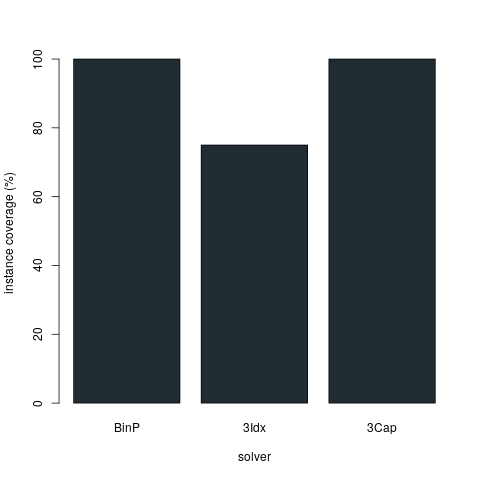
\includegraphics[width=1.2\textwidth]{img/solver_instance_coverage_b=3_s_3s.png}
\caption{\textsc{Zeitlimit} $3s$}
\label{fig:instance_coverage_b=3_s_a}
\end{subfigure}
\hfill
\begin{subfigure}[b]{0.3\textwidth}
\centering
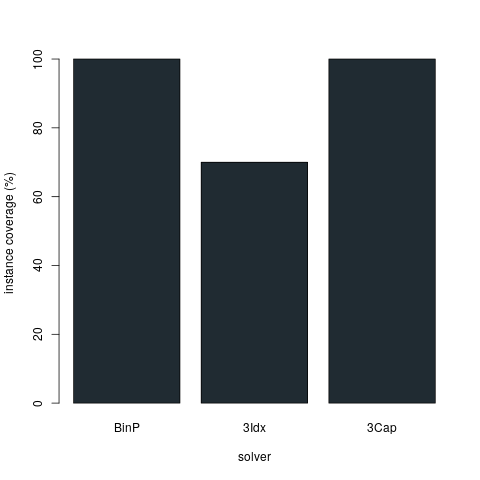
\includegraphics[width=1.2\textwidth]{img/solver_instance_coverage_b=3_s_5s.png}
\caption{\textsc{Zeitlimit} $5s$}
\label{fig:instance_coverage_b=3_s_b}
\end{subfigure}
\hfill
\begin{subfigure}[b]{0.3\textwidth}
\centering
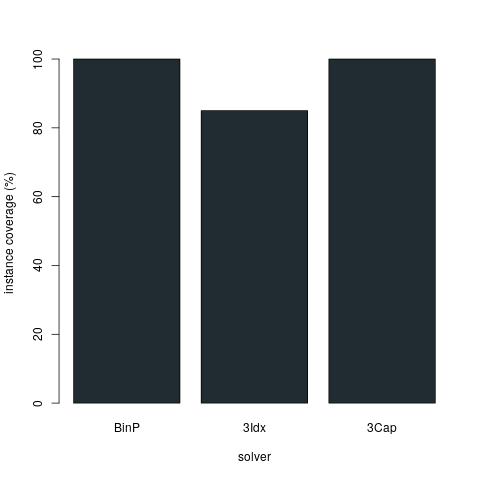
\includegraphics[width=1.2\textwidth]{img/solver_instance_coverage_b=3_s_10s.png}
\caption{\textsc{Zeitlimit} $10s$}
\label{fig:instance_coverage_b=3_s_c}
\end{subfigure}

\caption{}
\label{fig:instance_coverage_b=3_s}
\end{figure}

In der Darstellung der Laufzeiten in Abb. \ref{fig:b=3_s_runtimes} ist zu erkennen, dass die Bin-Packing-
und die 3-Index-Formulierung häufig ähnliche Laufzeiten besitzen. Da die 3-Index-Formulierung mit den Instanzen
$03, 09, 10, 11$ und $13$ allerdings einige Ausreißer, die eine deutlich längere Laufzeit erfordern, zeigt,
ist die Bin-Packing-Formulierung im Durchschnitt klar schneller.
Die Heuristik unterbietet diese mit einer durchschnittlichen Laufzeit von $0.01s$ allerdings noch einmal deutlich
und weicht dabei um durchschnittlich $2.65 \%$ vom Optimum ab.

Da die Bin-Packing-Formulierung, wie in Abb. \ref{fig:b=3_s_runtimes} zu erkennen ist, stets vor dem Zeitlimit terminiert,
wurden sämtliche Instanzen optimal gelöst. Die 3-Index-Formulierung wird basierend auf der Abbildung in drei Fällen
durch das Zeitlimit gestoppt. Wie man in Abb. \ref{fig:b=3_s_costs} erkennen kann, wurden mit den Instanzen $03$ und $11$
zwei der drei Fälle nicht optimal gelöst. In diesen Fällen kommt, wie man sieht, sogar die Heuristik zu besseren Zielfunktionswerten.
Im dritten Fall, in welchem die 3-Index-Formulierung durch das Zeitlimit gestoppt wurde, der Instanz $09$, hat diese
offenkundig lediglich noch nicht bewiesen, dass es sich um das Optimum handelt, der entsprechende Wert wurde allerdings,
wie man Abb. \ref{fig:b=3_s_costs} entnehmen kann, bereits ermittelt. Sofern beide MIP-Formulierungen den Optimalwert ermittelt haben,
verdecken die Einträge der 3-Index-Formulierung in der Abb. jeweils die Einträge der Bin-Packing-Formulierung.

\begin{figure}[H]
\centering
\begin{subfigure}[b]{0.4\textwidth}
\centering
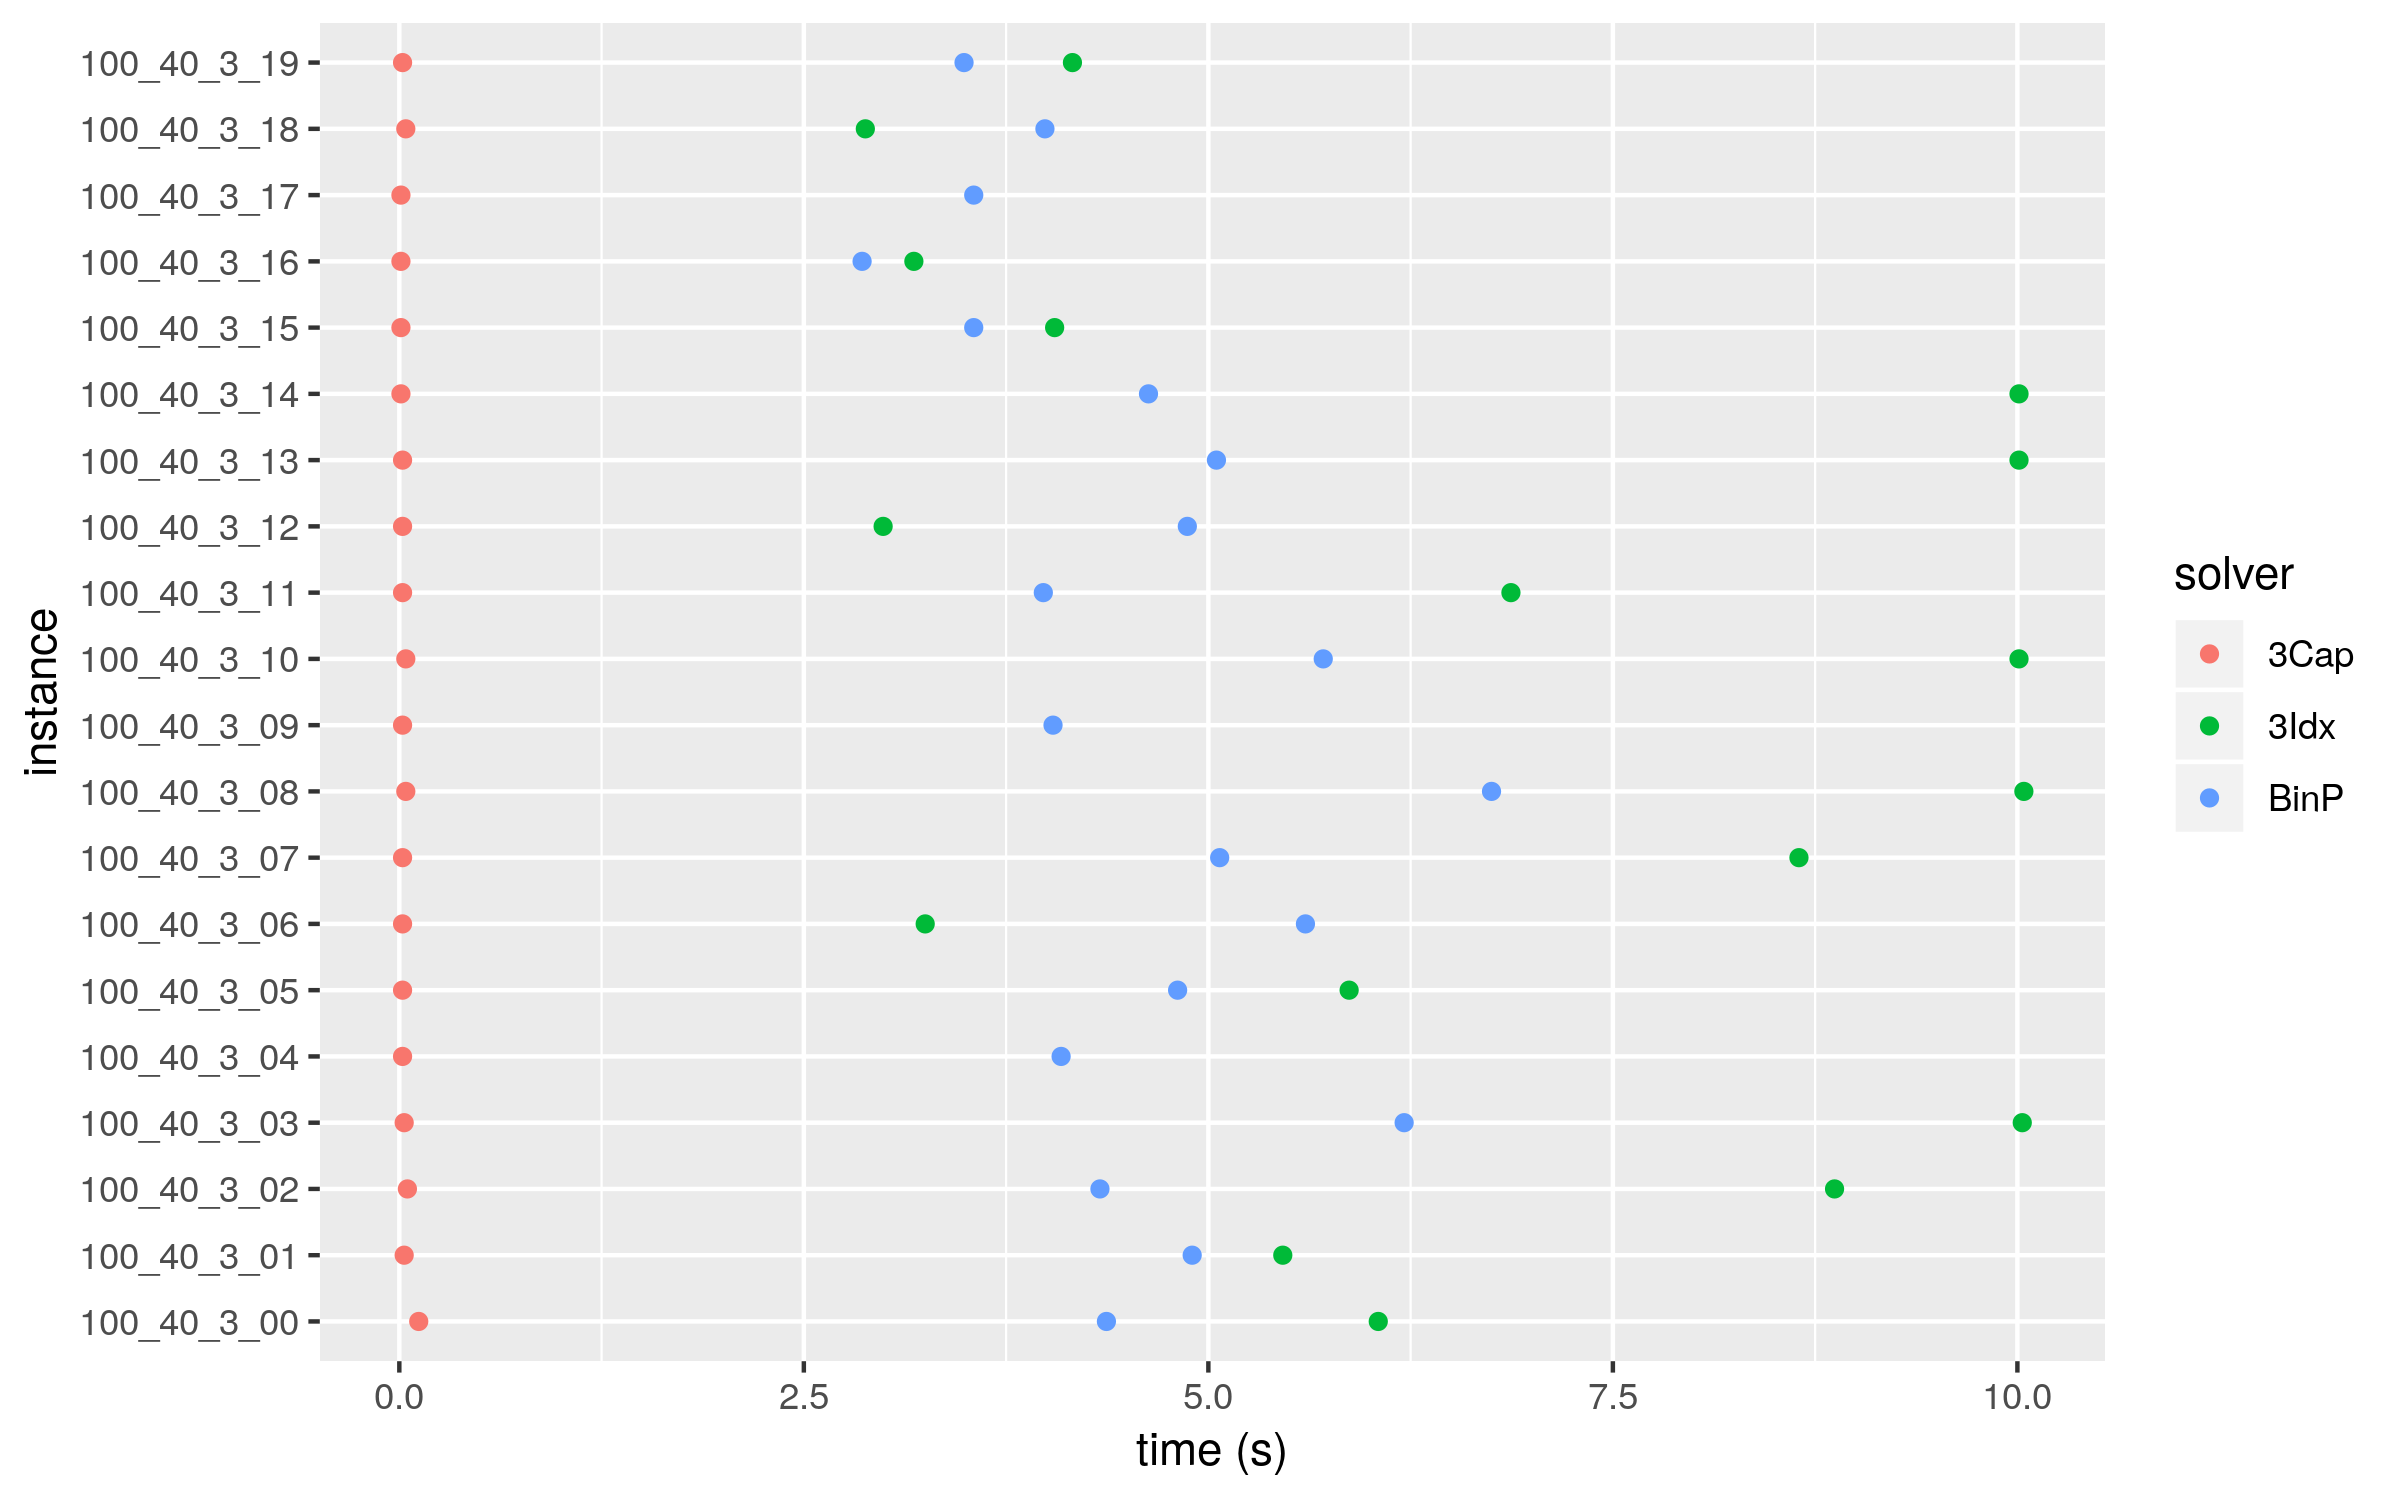
\includegraphics[width=1.3\textwidth]{img/solver_instance_time_b=3_s_10s.png}
\caption{\textsc{Laufzeiten bei 10s Zeitlimit}}
\label{fig:b=3_s_runtimes}
\end{subfigure}
\hfill
\begin{subfigure}[b]{0.4\textwidth}
\centering
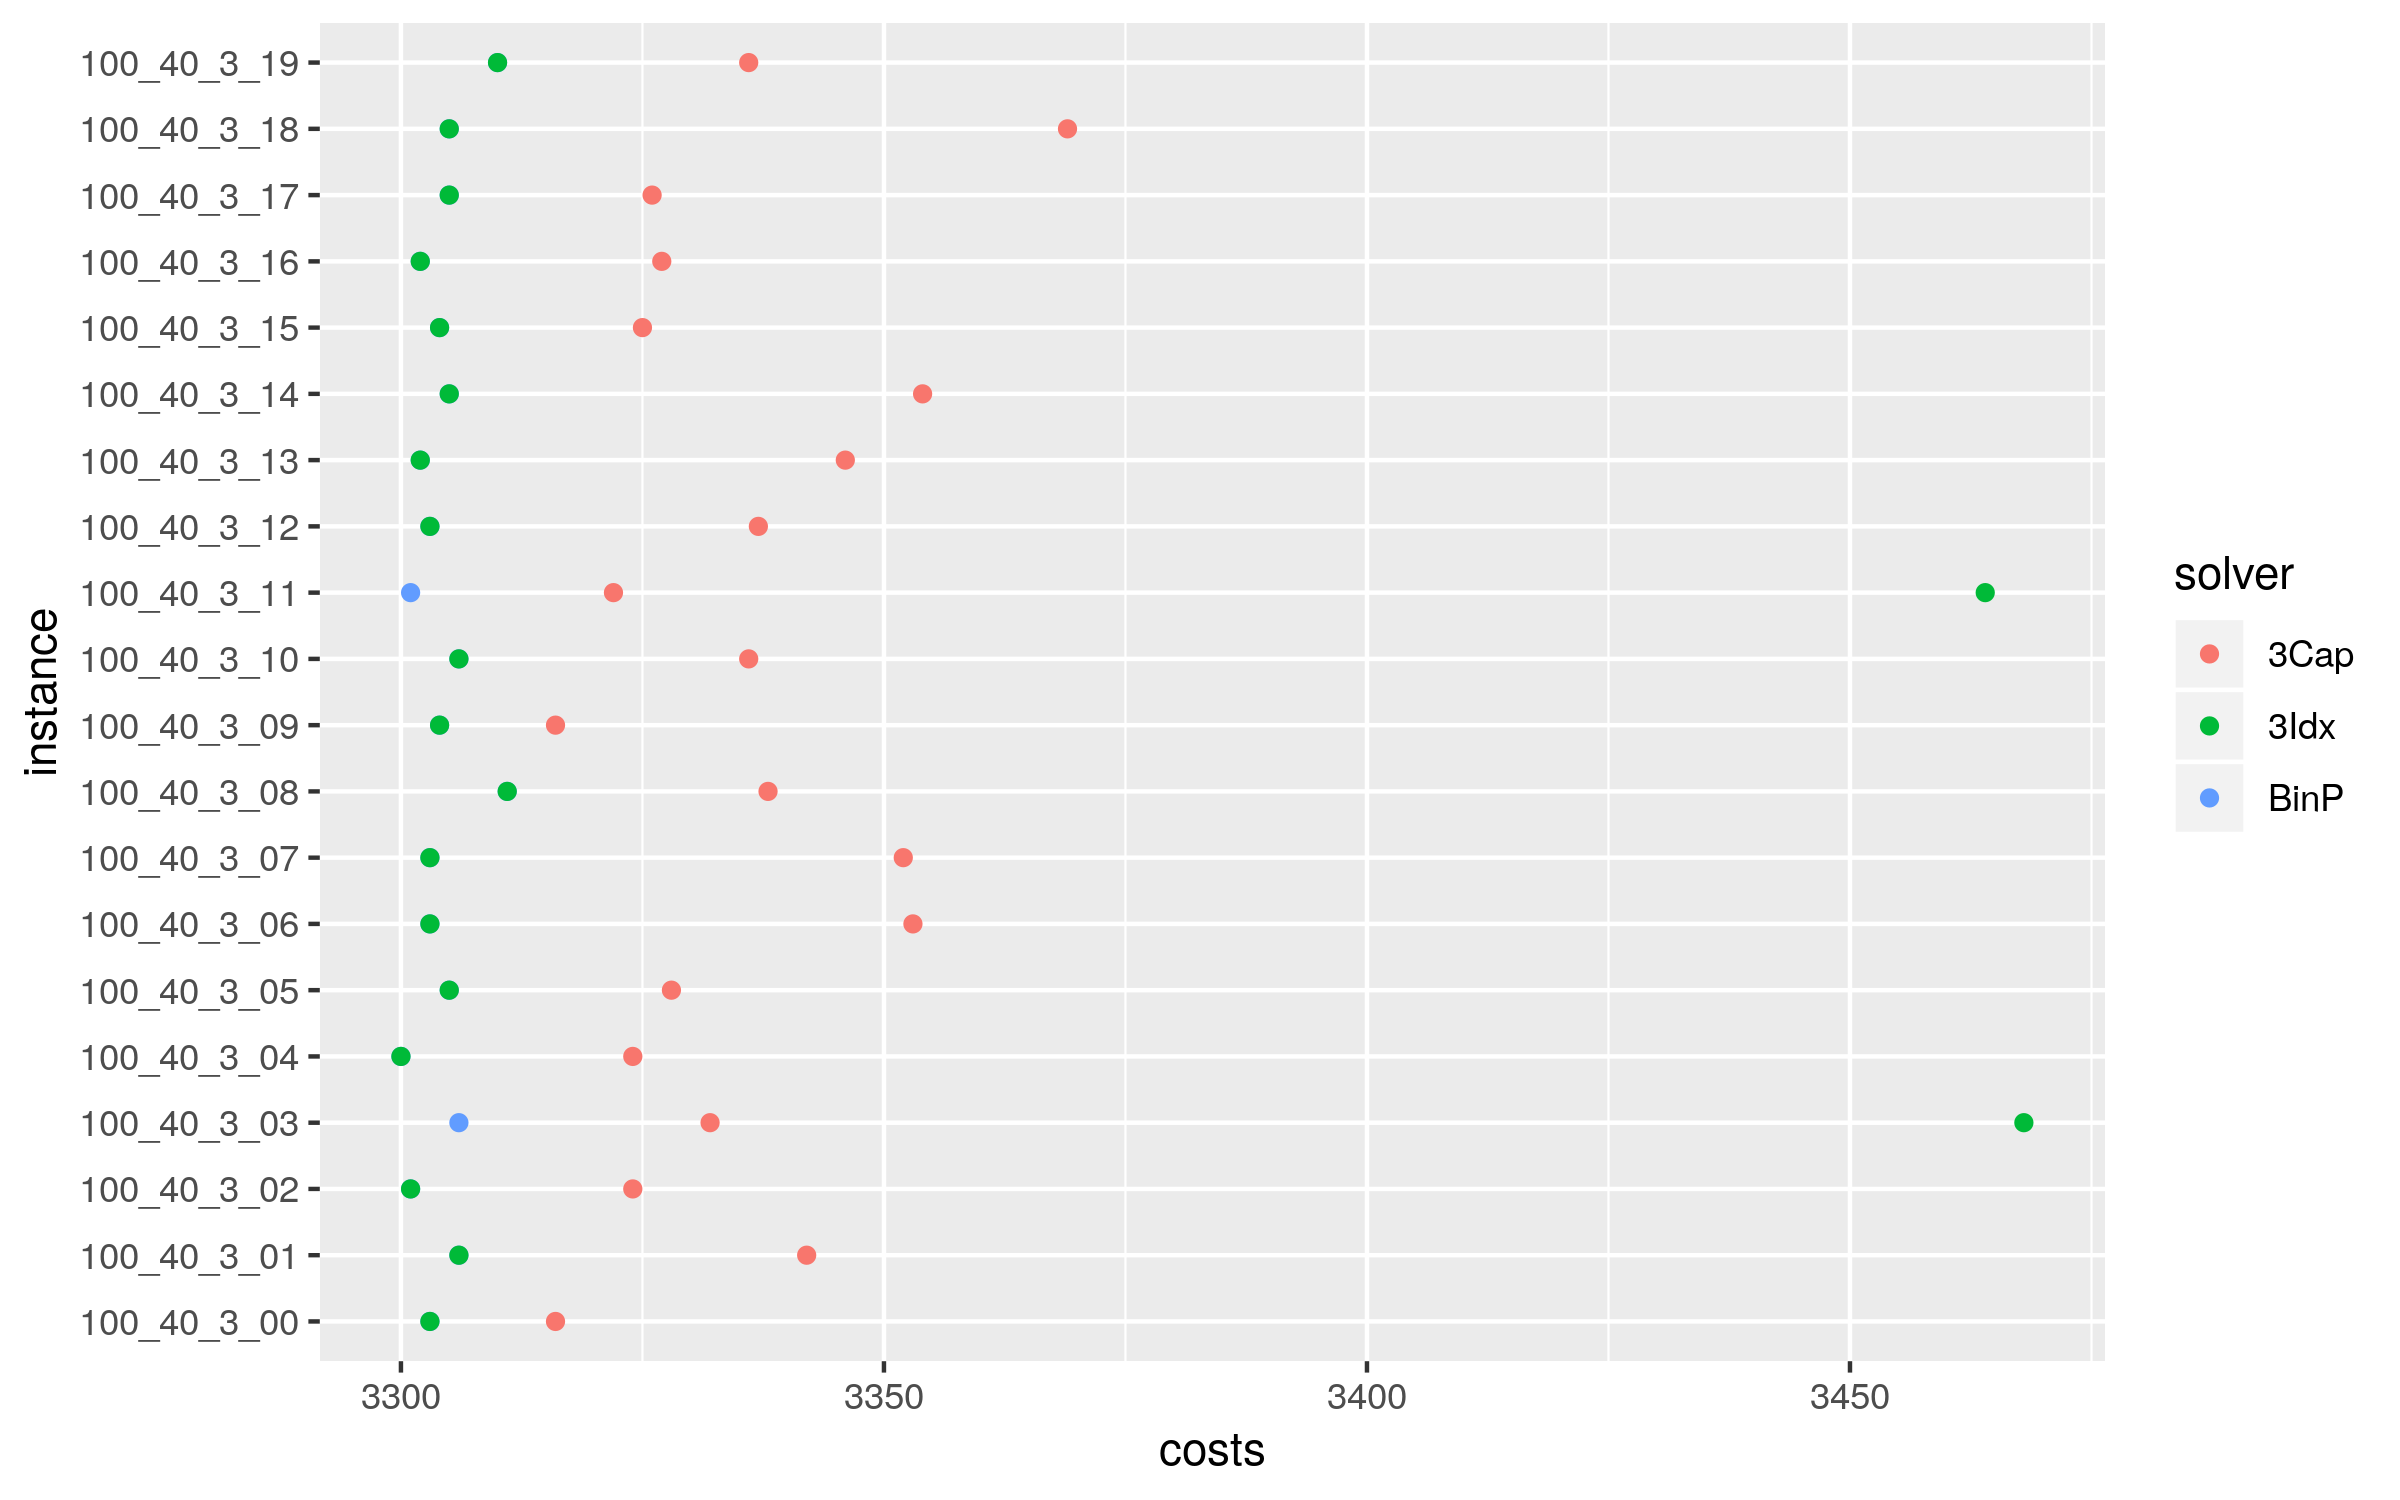
\includegraphics[width=1.3\textwidth]{img/solver_instance_cost_b=3_s_10s.png}
\caption{\textsc{Kosten bei 10s Zeitlimit}}
\label{fig:b=3_s_costs}
\end{subfigure}
\caption{}
\end{figure}

Abbildung \ref{fig:mip_results_b=3_s} ist zu entnehmen, dass die Bin-Packing-Formulierung nach durchschnittlich
$3.1s$ sämtliche Instanzen optimal löst. Bei einem Zeitlimit von $10s$ löst die 3-Index-Formulierung zwar ebenfalls
sämtliche Instanzen, allerdings nur $85 \%$ optimal. Dafür benötigt diese eine durchschnittliche Laufzeit von
$5.6s$. Wie bereits erwähnt, ist die Bin-Packing-Formulierung der 3-Index-Formulierung damit in dieser Kategorie vorzuziehen.

\begin{figure}[H]
\centering
\begin{subfigure}[b]{0.3\textwidth}
\centering
\resizebox{\textwidth}{!}{
\begin{tabular}{ | l | l | l |}
    \hline
     & \textbf{BinP} & \textbf{3Idx} \\ \hline
    \textbf{Optimal} & $\textcolor{mygreen}{40 \%}$ & $\textcolor{red}{5 \%}$ \\ \hline
    \textbf{Laufzeit} & \O $\thinspace 2.9 s$ & \O $\thinspace 2.9 s$ \\ \hline
    \textbf{Abweichung} & \O $\thinspace \textcolor{mygreen}{1.7 \%}$ & \O $\thinspace \textcolor{red}{7.8 \%}$ \\ \hline
\end{tabular}}
\caption{\textsc{Zeitlimit} $3s$}
\label{}
\end{subfigure}
% \end{figure}
% \begin{figure}[H]
\begin{subfigure}[b]{0.3\textwidth}
\centering
\resizebox{\textwidth}{!}{
\begin{tabular}{ | l | l | l |}
    \hline
     & \textbf{BinP} & \textbf{3Idx} \\ \hline
    \textbf{Optimal} & $\textcolor{mygreen}{100 \%}$ & $\textcolor{red}{50 \%}$ \\ \hline
    \textbf{Laufzeit} & \O $\thinspace \textcolor{mygreen}{3.1 s}$ & \O $\thinspace \textcolor{red}{4.0 s}$ \\ \hline
    \textbf{Abweichung} & \O $\thinspace \textcolor{mygreen}{0.0 \%}$ & \O $\thinspace \textcolor{red}{1.2 \%}$ \\ \hline
\end{tabular}}
\caption{\textsc{Zeitlimit} $5s$}
\label{}
\end{subfigure}
\begin{subfigure}[b]{0.3\textwidth}
\centering
\resizebox{\textwidth}{!}{
\begin{tabular}{ | l | l | l |}
    \hline
     & \textbf{BinP} & \textbf{3Idx} \\ \hline
    \textbf{Optimal} & $ \textcolor{mygreen}{100 \%}$ & $ \textcolor{red}{85 \%}$ \\ \hline
    \textbf{Laufzeit} & \O $\thinspace \textcolor{mygreen}{3.1 s}$ & \O $\thinspace \textcolor{red}{5.6 s}$ \\ \hline
    \textbf{Abweichung} & \O $\thinspace \textcolor{mygreen}{0.0 \%}$ & \O $\thinspace \textcolor{red}{0.5 \%}$ \\ \hline
\end{tabular}}
\caption{\textsc{Zeitlimit} $10s$}
\label{}
\end{subfigure}
\caption{\textsc{MIP-Ergebnisse.}}
\label{fig:mip_results_b=3_s}
\end{figure}

Bei der durchschnittlichen Abweichung der Heuristik von $2.65 \%$ handelt es sich sicher in Anbetracht
der enormen Laufzeitverbesserung um einen akzeptablen Wert, allerdings gilt, wie schon in der Kategorie
der kleinen Instanzen für eine Stack-Kapazität von $b = 2$ auch hier, dass die durchschnittlich benötigten $3.1s$
für die exakte Lösung seitens der Bin-Packing-Formulierung aus praktischer Perspektive vermutlich vertretbar sind
und kein wirklicher Bedarf für eine Laufzeitvebessrung durch eine Heuristik herrscht.

\textbf{Mittelgroße Instanzen (m)}

In der Kategorie der mittelgroßen Instanzen wurden Zeitlimits von $10$, $20$ und $30$ Minuten betrachtet.
In Abb. \ref{fig:instance_coverage_b=3_m} ist klar zu erkennen, dass die Bin-Packing-Formulierung hier erfolgsversprechender
als die 3-Index-Formulierung ist, welche selbst bei einem Zeitlimit von $30$ Minuten nur $40 \%$ der Instanzen löst
(vgl. Abb. \ref{fig:instance_coverage_b=3_m_c}). Die Bin-Packing-Formulierung löst, wie in Abb. \ref{fig:instance_coverage_b=3_m_b} zu sehen
ist, bereits bei einem Zeitlimit von $20$ Minuten sämtliche Instanzen.
Die Heuristik löst, wie zuvor, bei jedem Zeitlimit sämtliche Instanzen.

\begin{figure}[H]
\centering

\begin{subfigure}[b]{0.3\textwidth}
\centering
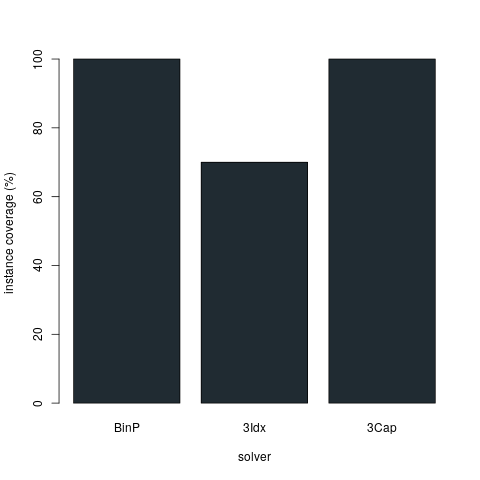
\includegraphics[width=1.2\textwidth]{img/solver_instance_coverage_b=3_m_600s.png}
\caption{\textsc{Zeitlimit} $10min$}
\label{fig:instance_coverage_b=3_m_a}
\end{subfigure}
\hfill
\begin{subfigure}[b]{0.3\textwidth}
\centering
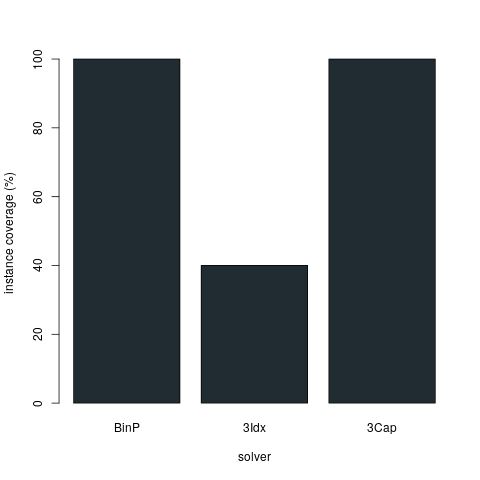
\includegraphics[width=1.2\textwidth]{img/solver_instance_coverage_b=3_m_1200s.png}
\caption{\textsc{Zeitlimit} $20min$}
\label{fig:instance_coverage_b=3_m_b}
\end{subfigure}
\hfill
\begin{subfigure}[b]{0.3\textwidth}
\centering
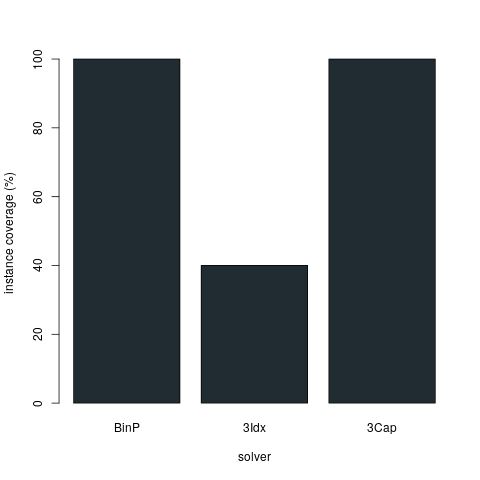
\includegraphics[width=1.2\textwidth]{img/solver_instance_coverage_b=3_m_1800s.png}
\caption{\textsc{Zeitlimit} $30min$}
\label{fig:instance_coverage_b=3_m_c}
\end{subfigure}

\caption{}
\label{fig:instance_coverage_b=3_m}
\end{figure}

In Abb. \ref{fig:b=3_m_runtimes} ist zu sehen, dass die 3-Index-Formulierung nur für 8 der 20 Instanzen
bei einem Zeitlimit von einer halben Stunde überhaupt zu einer Lösung gelangt, daraus ergibt sich die Instance-Coverage
von $40 \%$. Bei den Instanzen, die auch von der 3-Index-Formulierung gelöst wurden, unterscheiden sich die Laufzeiten
nur marginal von denen der Bin-Packing-Formulierung, wenngleich diese im Durchschnitt trotzdem etwas schneller ist.

Die Heuristik ist, wie auch in Abb. \ref{fig:b=3_m_runtimes} klar wird, noch einmal erheblich schneller.
Mit einer durchschnittlichen Laufzeit von nur $0.2s$ löst diese sämtliche Instanzen und unterbietet die MIP-Formulierungen
damit um mehrere Größenordnungen.

Für die Kosten gilt, wie man Abb. \ref{fig:b=3_m_costs} entnehmen kann, dass die Heuristik, wie in vorherigen Experimenten,
eine Abweichung von den Optimalwerten der MIP-Formulierungen im einstelligen Prozentbereich besitzt.

\begin{figure}[H]
\centering
\begin{subfigure}[b]{0.4\textwidth}
\centering
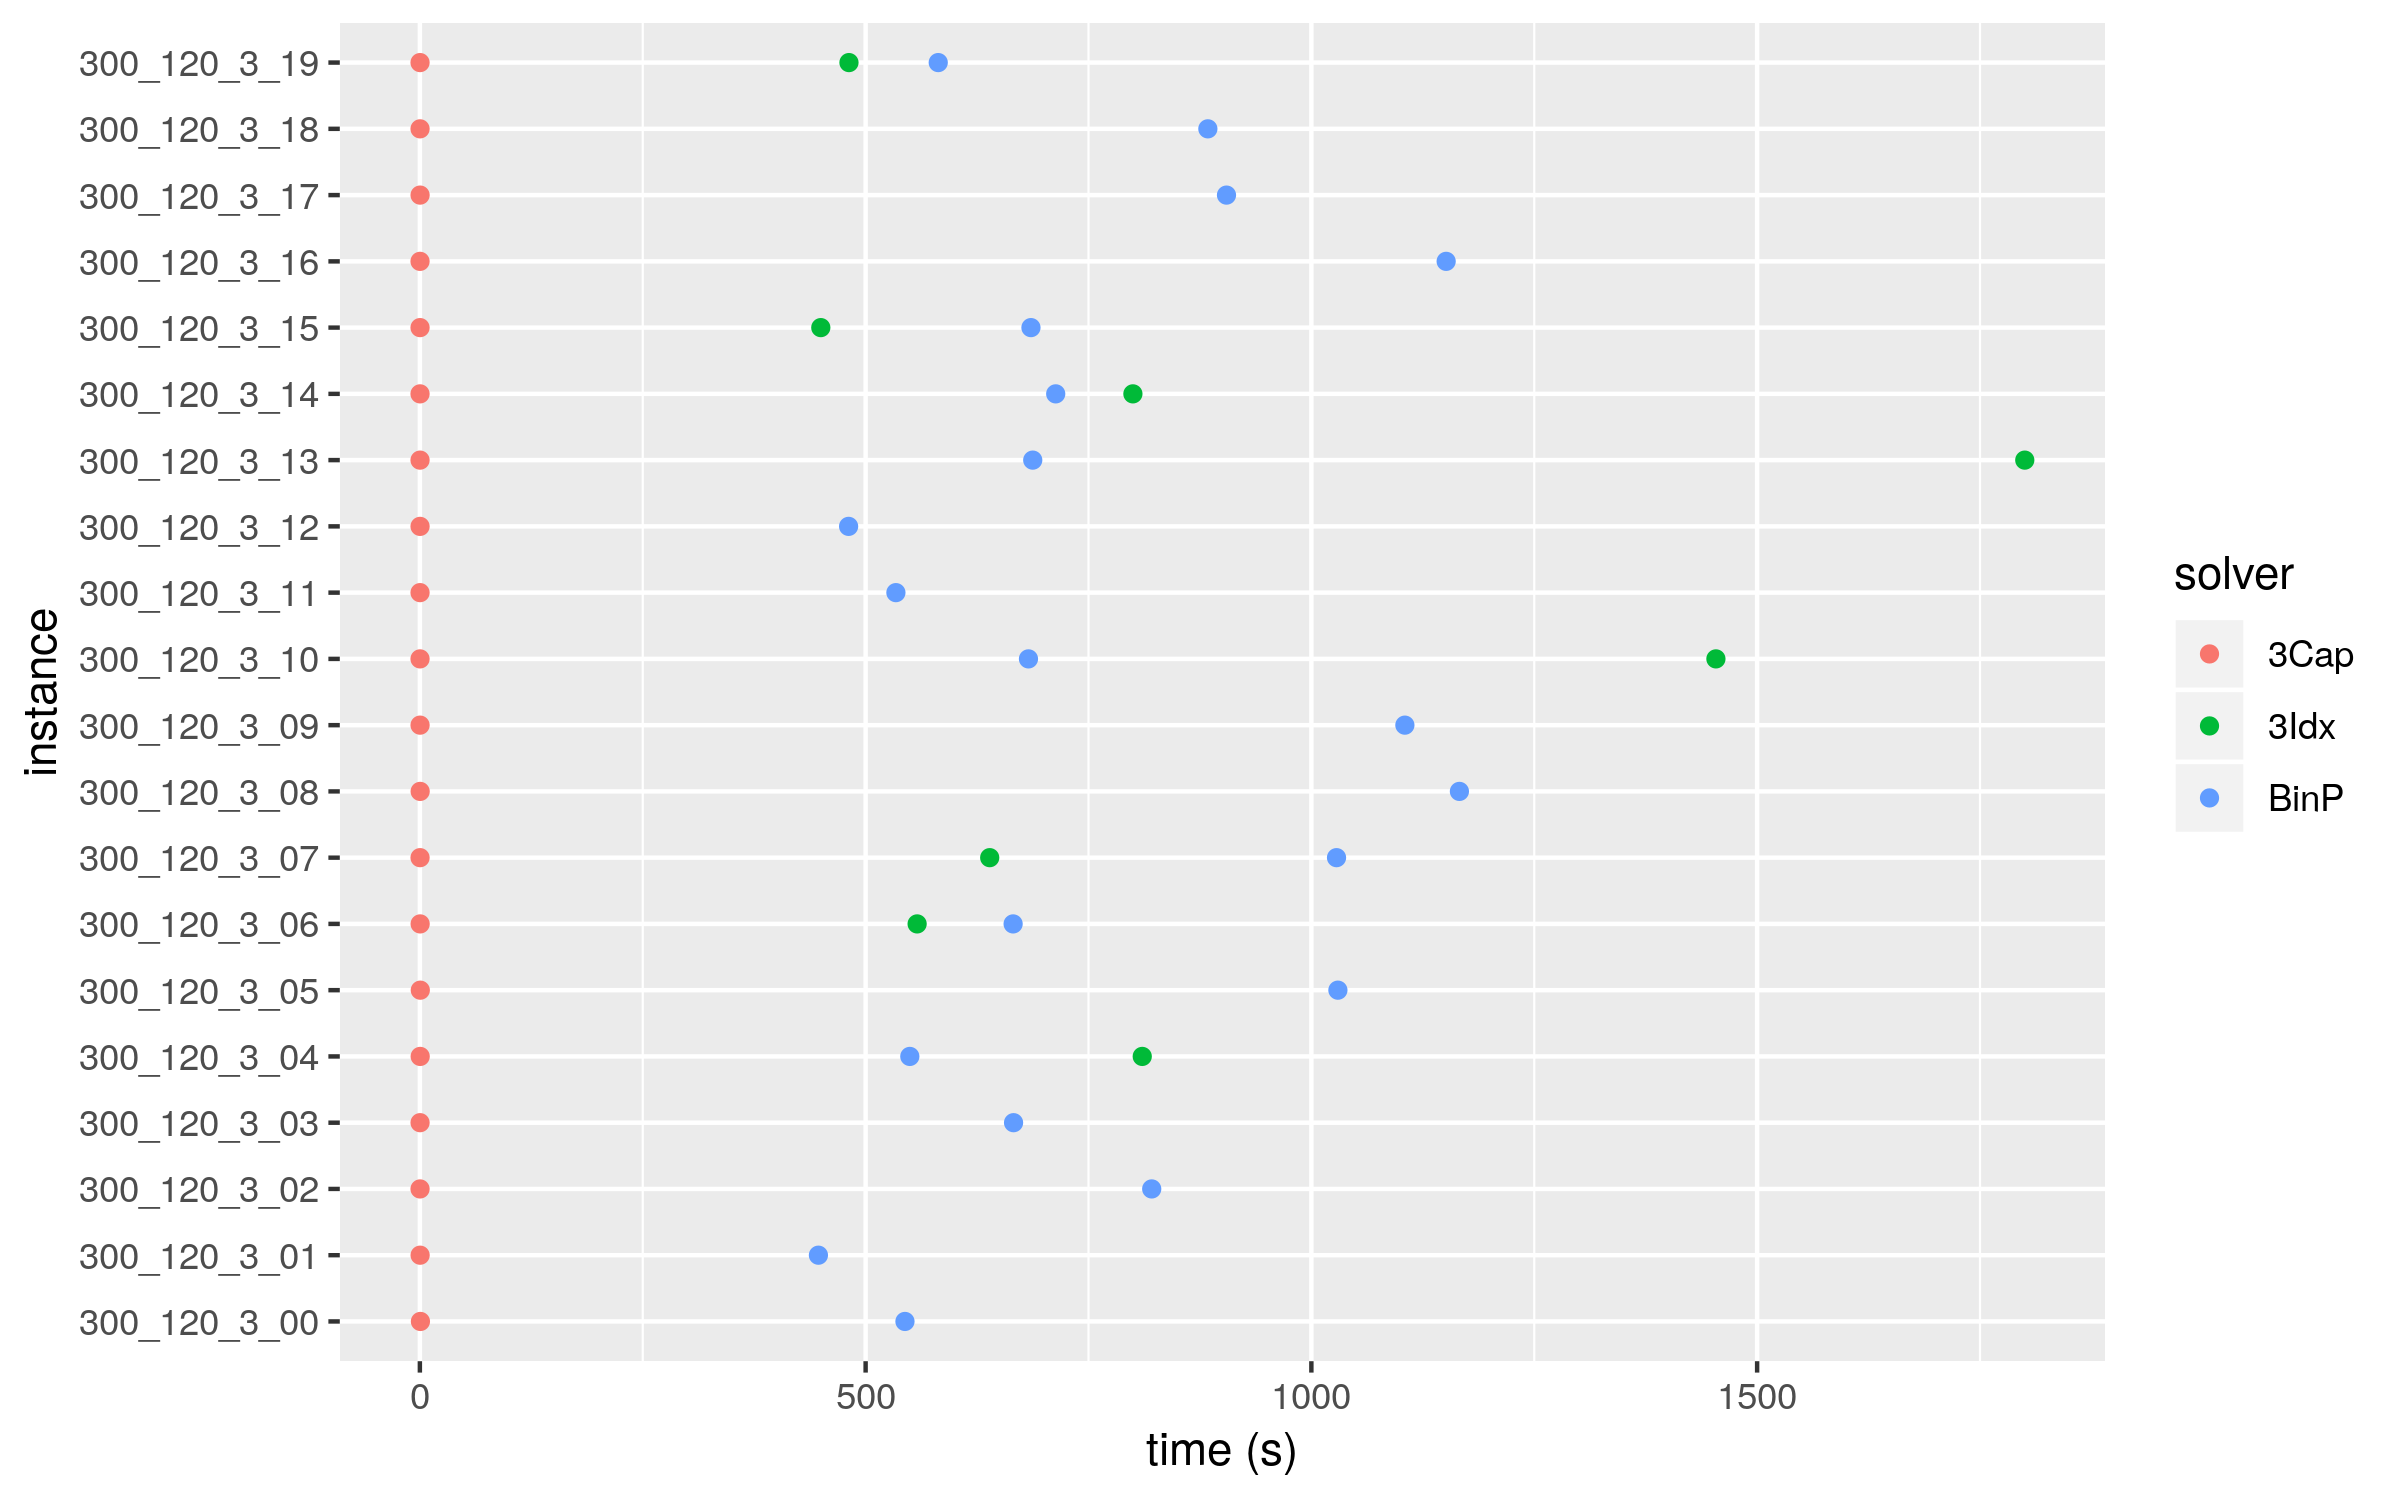
\includegraphics[width=1.3\textwidth]{img/solver_instance_time_b=3_m_1800s.png}
\caption{\textsc{Laufzeiten bei 30min Limit}}
\label{fig:b=3_m_runtimes}
\end{subfigure}
\hfill
\begin{subfigure}[b]{0.4\textwidth}
\centering
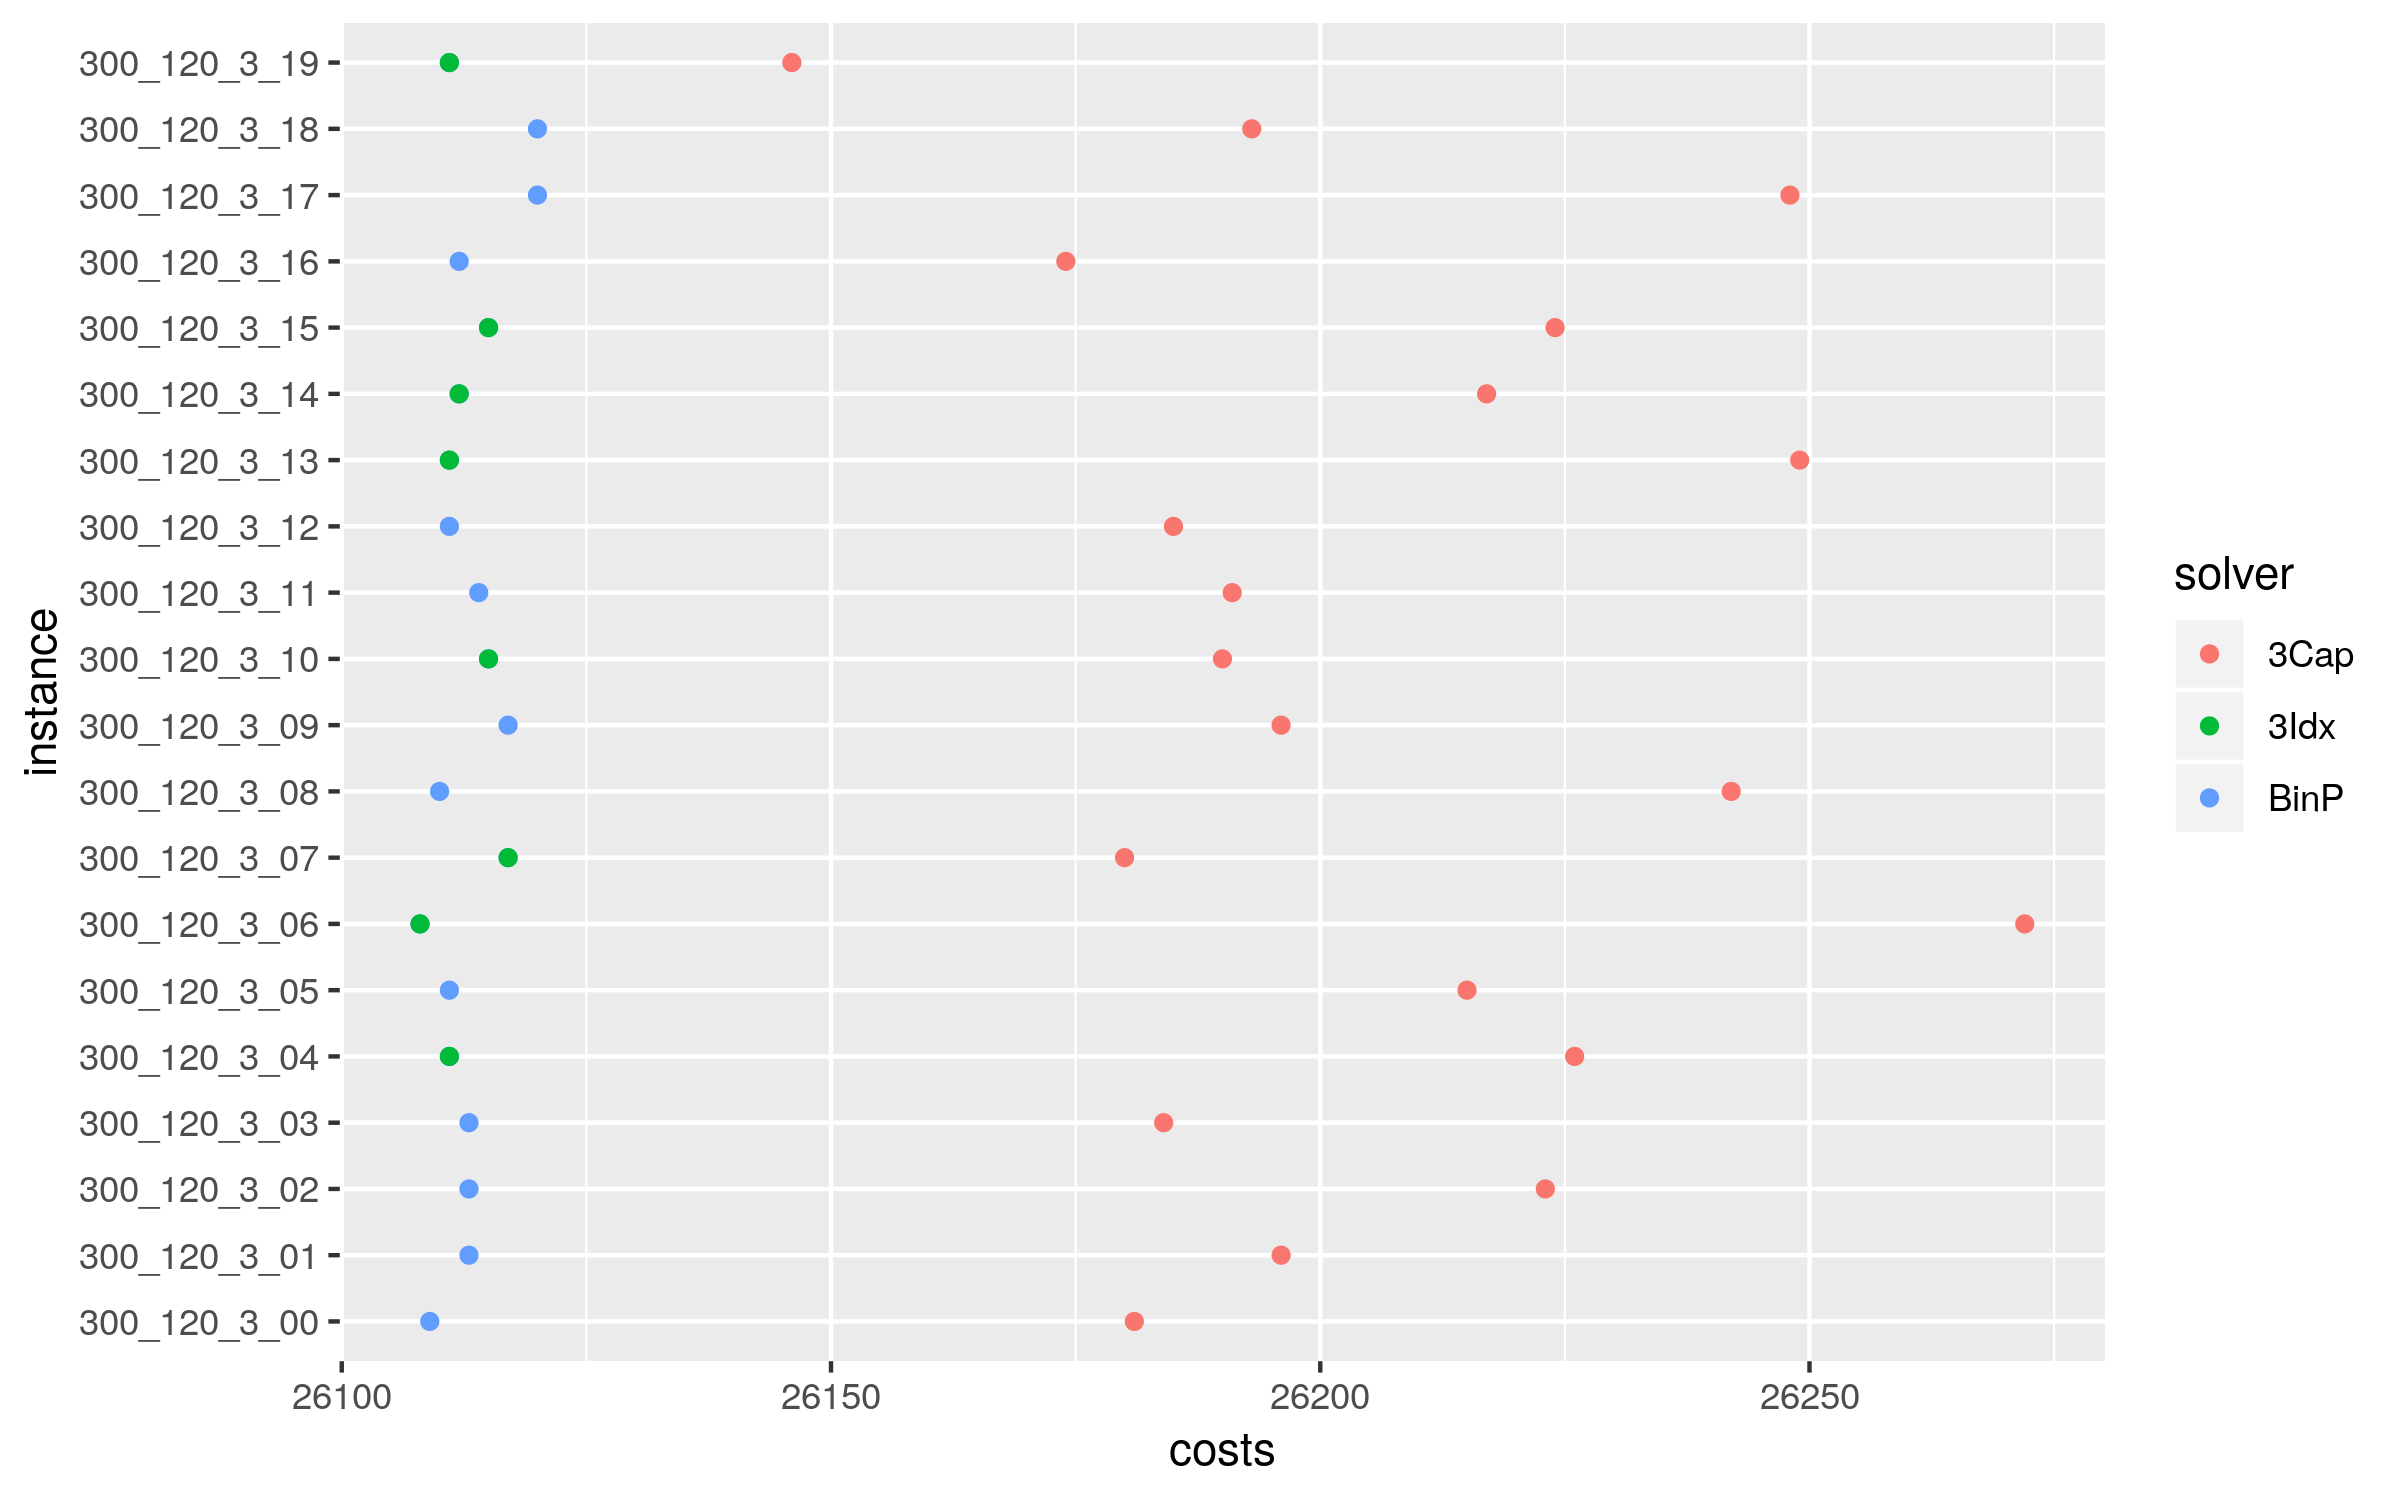
\includegraphics[width=1.3\textwidth]{img/solver_instance_cost_b=3_m_1800s.png}
\caption{\textsc{Kosten bei 30min Limit}}
\label{fig:b=3_m_costs}
\end{subfigure}
\caption{}
\end{figure}

Abbildung \ref{fig:mip_results_b=3_m_a} bestätigt die Tendenz der Visualisierungen der Instance-Coverage und belegt,
dass beide MIP-Formulierungen bei einem Zeitlimit von $10$ Minuten nur wenige Instanzen überhaupt und noch weniger
Instanzen optimal lösen.
Besser wird es bei einem Zeitlimit von $20$ Minuten, bei welchem die Bin-Packing-Formulierung mit einer durchschnittlichen
Laufzeit von ca. $13$ Minuten sämtliche Instanzen optimal löst. Somit ist diese der 3-Index-Formulierung hier klar zu bevorzugen,
die selbst bei einem Zeitlimit von $30$ Minuten nur $35 \%$ der Instanzen optimal löst (vlg. Abb. \ref{fig:mip_results_b=3_m_b},
\ref{fig:mip_results_b=3_m_c}).

Die Heuristik benötigt durchschnittlich eine Laufzeit von nur $0.2s$ und weicht dabei um durchschnittlich
$1.02 \%$ vom Optimum ab. Wie bereits im $b = 2$ Szenario, ist dieser erhebliche Laufzeitunterschied
um mehrere Größenordnungen wohl hinreichende Motivation, um diese jeweils geringe Abweichung vom Optimum in Kauf zu nehmen.

\begin{figure}[H]
\begin{subfigure}[b]{0.3\textwidth}
\centering
\resizebox{\textwidth}{!}{
\begin{tabular}{ | l | l | l |}
    \hline
     & \textbf{BinP} & \textbf{3Idx} \\ \hline
    \textbf{Optimal} & $ \textcolor{mygreen}{20 \%}$ & $ \textcolor{red}{10 \%}$ \\ \hline
    \textbf{Laufzeit} & \O $\thinspace \textcolor{red}{583.7 s}$ & \O $\thinspace \textcolor{mygreen}{554.3 s}$ \\ \hline
    \textbf{Abweichung} & \O $\thinspace \textcolor{red}{0.2 \%}$ & \O $\thinspace \textcolor{mygreen}{0.01 \%}$ \\ \hline
\end{tabular}}
\caption{\textsc{Zeitlimit} $10min$}
\label{fig:mip_results_b=3_m_a}
\end{subfigure}
% $\quad\quad\quad\quad$
\begin{subfigure}[b]{0.3\textwidth}
\centering
\resizebox{\textwidth}{!}{
\begin{tabular}{ | l | l | l |}
    \hline
     & \textbf{BinP} & \textbf{3Idx} \\ \hline
    \textbf{Optimal} & $ \textcolor{mygreen}{100 \%}$ & $ \textcolor{red}{30 \%}$ \\ \hline
    \textbf{Laufzeit} & \O $\thinspace \textcolor{mygreen}{791.4 s}$ & \O $\thinspace \textcolor{red}{795.4 s}$ \\ \hline
    \textbf{Abweichung} & \O $\thinspace 0.0 \%$ & \O $\thinspace 0.0 \%$ \\ \hline
\end{tabular}}
\caption{\textsc{Zeitlimit} $20min$}
\label{fig:mip_results_b=3_m_b}
\end{subfigure}
% \end{figure}
% \begin{figure}[H]
\begin{subfigure}[b]{0.3\textwidth}
\centering
\resizebox{\textwidth}{!}{
\begin{tabular}{ | l | l | l |}
    \hline
     & \textbf{BinP} & \textbf{3Idx} \\ \hline
    \textbf{Optimal} & $ \textcolor{mygreen}{100 \%}$ & $ \textcolor{red}{35 \%}$ \\ \hline
    \textbf{Laufzeit} & \O $\thinspace \textcolor{mygreen}{766.4 s}$ & \O $\thinspace \textcolor{red}{874.0 s}$ \\ \hline
    \textbf{Abweichung} & \O $\thinspace 0.0 \%$ & \O $\thinspace 0.0 \%$ \\ \hline
\end{tabular}}
\caption{\textsc{Zeitlimit} $30min$}
\label{fig:mip_results_b=3_m_c}
\end{subfigure}

\caption{\textsc{MIP-Ergebnisse.}}
\label{fig:mip_results_b=3_m}
\end{figure}

\pagebreak

\textbf{Große Instanzen (l)}

Zuletzt werden die Solver für die in Kapitel \ref{sec:instance_sizes} als groß bezeichneten Instanzen,
bei denen es darum geht, 500 eintreffende Items in die Storage-Area zu verladen, verglichen.
In dieser Kategorie werden Zeitlimits von $15, 30$ und $45$ Minuten betrachtet.

\begin{figure}[H]
\centering

\begin{subfigure}[b]{0.3\textwidth}
\centering
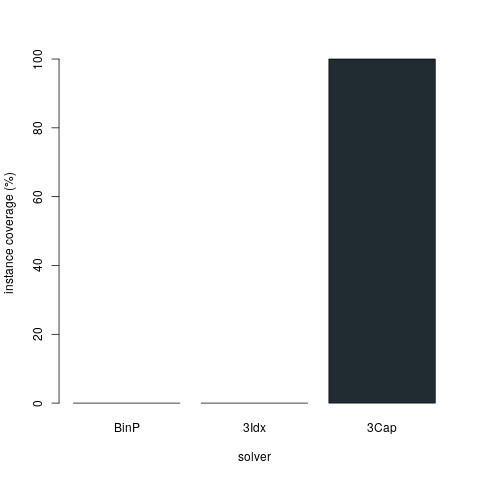
\includegraphics[width=1.2\textwidth]{img/solver_instance_coverage_b=3_l_1800s.png}
\caption{\textsc{Zeitlimit} $30min$}
\label{fig:instance_coverage_b=3_l_a}
\end{subfigure}
\hfill
\begin{subfigure}[b]{0.3\textwidth}
\centering
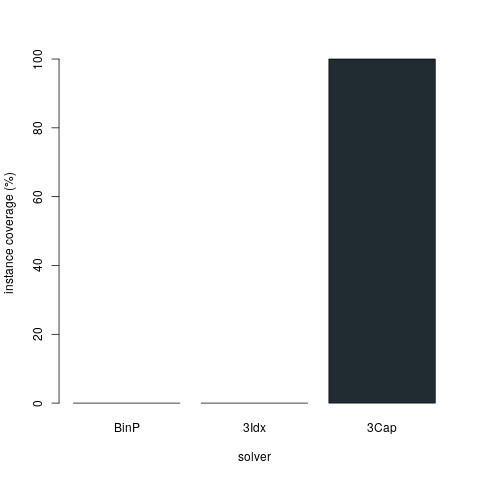
\includegraphics[width=1.2\textwidth]{img/solver_instance_coverage_b=3_l_2700s.png}
\caption{\textsc{Zeitlimit} $45min$}
\label{fig:instance_coverage_b=3_l_b}
\end{subfigure}
\hfill
\begin{subfigure}[b]{0.3\textwidth}
\centering

\includegraphics[width=1.2\textwidth]{img/na.png}
\caption{\textsc{Zeitlimit} $60min$}
\label{fig:instance_coverage_b=3_l_c}
\end{subfigure}

\caption{}
\label{}
\end{figure}

\begin{figure}[H]
\begin{subfigure}[b]{0.3\textwidth}
\centering
\resizebox{\textwidth}{!}{
\begin{tabular}{ | l | l | l |}
    \hline
     & \textbf{BinP} & \textbf{3Idx} \\ \hline
    \textbf{Optimal} & $ \textcolor{red}{0 \%}$ & $ \textcolor{red}{0 \%}$ \\ \hline
    \textbf{Laufzeit} & $\textcolor{red}{---}$ & $\textcolor{red}{---}$ \\ \hline
    \textbf{Abweichung} & $\textcolor{red}{---}$ & $\textcolor{red}{---}$ \\ \hline
\end{tabular}}
\caption{\textsc{Zeitlimit} $30min$}
\label{}
\end{subfigure}
% $\quad\quad\quad\quad$
\begin{subfigure}[b]{0.3\textwidth}
\centering
\resizebox{\textwidth}{!}{
\begin{tabular}{ | l | l | l |}
    \hline
     & \textbf{BinP} & \textbf{3Idx} \\ \hline
    \textbf{Optimal} & $ \textcolor{red}{0 \%}$ & $ \textcolor{red}{0 \%}$ \\ \hline
    \textbf{Laufzeit} & $\textcolor{red}{---}$ & $\textcolor{red}{---}$ \\ \hline
    \textbf{Abweichung} & $\textcolor{red}{---}$ &$\textcolor{red}{---}$ \\ \hline
\end{tabular}}
\caption{\textsc{Zeitlimit} $45min$}
\label{}
\end{subfigure}
% \end{figure}
% \begin{figure}[H]
\begin{subfigure}[b]{0.3\textwidth}
\centering
\resizebox{\textwidth}{!}{
\begin{tabular}{ | l | l | l |}
    \hline
     & \textbf{BinP} & \textbf{3Idx} \\ \hline
    \textbf{Optimal} & $-tbd-$ & $-tbd-$ \\ \hline
    \textbf{Laufzeit} & $-tbd-$ & $-tbd-$ \\ \hline
    \textbf{Abweichung} & $-tbd-$ & $-tbd-$ \\ \hline
\end{tabular}}
\caption{\textsc{Zeitlimit} $60min$}
\label{}
\end{subfigure}
\end{figure}

\pagebreak

\section{Verbesserungsverfahren}
\label{sec:post_optimization}

Bei Verbesserungsverfahren handelt es sich um lokale Suchverfahren, welche bereits mit einer Lösung des Problems starten,
die z.B. durch ein konstruktives Eröffnungsverfahren, wie den Heuristiken aus den Kapiteln \ref{sec:two_cap_heuristic} und \ref{sec:three_cap_heuristic} bestimmt wurden und versuchen diese im Laufe des Verfahrens zu verbessern.

Dabei wird zwischen deterministischen Verfahren, die bei gleichen Startlösungen und gleichen Rahmenbedingungen stets zum gleichen
Ergebnis kommen und stochastischen Verfahren, bei denen durch den Einsatz einer Zufallskomponente unterschiedliche Lösungen
generiert werden, unterschieden. \cite{Knust2017}

\textbf{Lokale Suchverfahren}

Bei den in dieser Arbeit betrachteten lokalen Suchverfahren handelt es sich um sogenannte Metaheuristiken,
weil sie nicht auf ein spezielles Problem abzielen, sondern auf grundsätzlichen Suchprinzipien beruhen,
die auf eine Vielzahl von Optimierungsproblemen anwendbar sind.
Das ist auch direkt einer der Gründe, weshalb sich diese Heuristiken einer so großen Beliebtheit erfreuen,
sie sind allgemein anwendbar und sehr flexibel an konkrete Problemstellungen anpassbar.

Die Idee eines lokalen Suchverfahrens ist es, ausgehend von der Initiallösung, durch wohldefinierte Regeln zu anderen,
verbessernden Lösungen innerhalb der Nachbarschaft zu gelangen. Dazu muss die Struktur dieser Nachbarschaft zunächst
klar definiert werden. Wurde eine solche verbessernde Lösung gefunden, so wird entsprechend deren Nachbarschaft
nach verbessernden Lösungen durchsucht.
Das Kriterium, anhand dessen die jeweils nächste Lösung ausgewählt wird, entspricht häufig der besten Lösung.
Dabei wird solange fortgeschritten, bis keine bessere Lösung in der Nachbarschaft gefunden wird.

Dabei hängt der Erfolg dieses Ansatzes und somit die Lösungsqualität primär von der definierten Struktur der Nachbarschaft ab.

Der größte Schwäche dieses Ansatzes ist die Unfähigkeit, lokale Minima zu verlassen. Dieses Problem ist sehr
anschaulich in Abb. \ref{} visualisiert. Darin sind sämtliche Lösungen in der Nachbarschaft schlechter
als die gegenwärtige Lösung, obwohl weiter entfernt ein globales Minimum existiert, welches
basierend auf der ... nicht erreicht werden kann.

\begin{figure}[H]
\centering
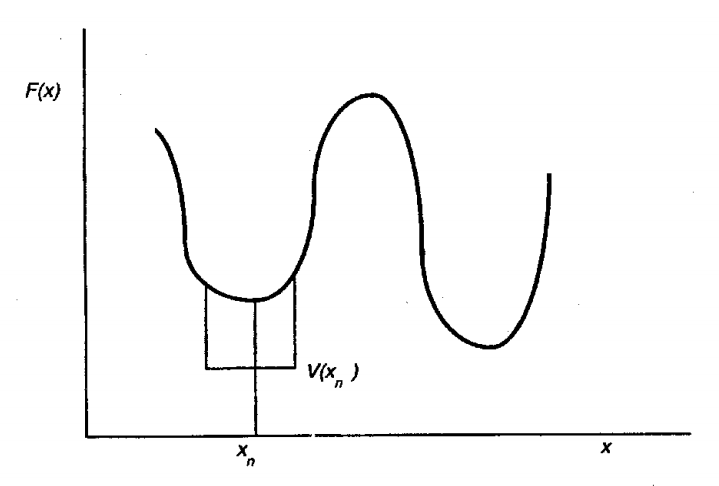
\includegraphics[width=0.7\textwidth]{img/local_minimum.png}
\caption{Schwäche lokaler Suchverfahren. \cite{Pirlot1996}}
\label{}
\end{figure}

\textbf{Formaler Ablauf einer lokalen Suche}

Eine lokale Suche startet mit einer beliebigen Lösung $x_1 \in X$ und in jedem Schritt $n$
wird eine neue Lösung $x_{n+1}$ aus der Nachbarschaft $V(x_n)$ der gegenwärtigen Lösung $x_n$ gewählt.
Für jedes $x \in X$ existiert also eine solche Nachbarschaft $V(x) \subseteq X$.

Ein simples Beispiel für eine solche Nachbarschaft ist ein Bitvektor. Wenn $X$ also eine Menge
von Bitvektoren ist und $x \in X$, dann kann eine Nachbarschaft $V(x)$ von $x$ als die Menge
sämtlicher Lösungen $x \in X$ definiert werden, bei denen in $x$ ein einzelnes Bit geflippt wird.

Typischerweise entspricht das Kriterium, anhand welchem die nächste Lösung $x_{n+1}$ gewählt wird,
die beste Lösung in der Nachbarschaft von $x_n$ zu wählen, also eine Lösung $x_{n+1} \in V(x_n)$
mit $F(x_{n+1}) \leq F(x) \forall x \in V(x_n)$.

Sollte dabei keine verbessernde Lösung in der Nachbarschaft gefunden werden, so terminiert die Suche.
Diese Strategien wird \textquote{Steepest Descent} genannt, also die Strategie des steilsten Abstiegs.
Dieser Name kommt daher, dass man bei einem Minimierungsproblem in der Richtung des steilsten Abstiegs
von der Initiallösung voranschreitet, bis man keine Verbesserung mehr erzielt.

\textbf{Beispiel}

Lösung $x$ kodiert als Bitvektor: $x = \{1, 1, 1, 0, 1, 0\}$.
Die Nachbarschaft dieser Lösung sieht nun wie folgt aus:\newline
\[
V(x) =
  \begin{bmatrix}
    \boldsymbol{0} & 1 & 1 & 0 & 1 & 0 \\
    1 & \boldsymbol{0} & 1 & 0 & 1 & 0 \\
    1 & 1 & \boldsymbol{0} & 0 & 1 & 0 \\
    1 & 1 & 1 & \boldsymbol{1} & 1 & 0 \\
    1 & 1 & 1 & 0 & \boldsymbol{0} & 0 \\
    1 & 1 & 1 & 0 & 1 & \boldsymbol{1}
  \end{bmatrix}
\]

\pagebreak

\section{Fazit}
\label{sec:conclusion}
